% Options for packages loaded elsewhere
\PassOptionsToPackage{unicode}{hyperref}
\PassOptionsToPackage{hyphens}{url}
\PassOptionsToPackage{dvipsnames,svgnames,x11names}{xcolor}
%
\documentclass[
  12pt,
  a4paper, twoside]{book}
\usepackage{amsmath,amssymb}
\usepackage{iftex}
\ifPDFTeX
  \usepackage[T1]{fontenc}
  \usepackage[utf8]{inputenc}
  \usepackage{textcomp} % provide euro and other symbols
\else % if luatex or xetex
  \usepackage{unicode-math} % this also loads fontspec
  \defaultfontfeatures{Scale=MatchLowercase}
  \defaultfontfeatures[\rmfamily]{Ligatures=TeX,Scale=1}
\fi
\usepackage{lmodern}
\ifPDFTeX\else
  % xetex/luatex font selection
\fi
% Use upquote if available, for straight quotes in verbatim environments
\IfFileExists{upquote.sty}{\usepackage{upquote}}{}
\IfFileExists{microtype.sty}{% use microtype if available
  \usepackage[]{microtype}
  \UseMicrotypeSet[protrusion]{basicmath} % disable protrusion for tt fonts
}{}
\makeatletter
\@ifundefined{KOMAClassName}{% if non-KOMA class
  \IfFileExists{parskip.sty}{%
    \usepackage{parskip}
  }{% else
    \setlength{\parindent}{0pt}
    \setlength{\parskip}{6pt plus 2pt minus 1pt}}
}{% if KOMA class
  \KOMAoptions{parskip=half}}
\makeatother
\usepackage{xcolor}
\usepackage{longtable,booktabs,array}
\usepackage{calc} % for calculating minipage widths
% Correct order of tables after \paragraph or \subparagraph
\usepackage{etoolbox}
\makeatletter
\patchcmd\longtable{\par}{\if@noskipsec\mbox{}\fi\par}{}{}
\makeatother
% Allow footnotes in longtable head/foot
\IfFileExists{footnotehyper.sty}{\usepackage{footnotehyper}}{\usepackage{footnote}}
\makesavenoteenv{longtable}
\usepackage{graphicx}
\makeatletter
\def\maxwidth{\ifdim\Gin@nat@width>\linewidth\linewidth\else\Gin@nat@width\fi}
\def\maxheight{\ifdim\Gin@nat@height>\textheight\textheight\else\Gin@nat@height\fi}
\makeatother
% Scale images if necessary, so that they will not overflow the page
% margins by default, and it is still possible to overwrite the defaults
% using explicit options in \includegraphics[width, height, ...]{}
\setkeys{Gin}{width=\maxwidth,height=\maxheight,keepaspectratio}
% Set default figure placement to htbp
\makeatletter
\def\fps@figure{htbp}
\makeatother
\setlength{\emergencystretch}{3em} % prevent overfull lines
\providecommand{\tightlist}{%
  \setlength{\itemsep}{0pt}\setlength{\parskip}{0pt}}
\setcounter{secnumdepth}{5}
\ifLuaTeX
\usepackage[bidi=basic]{babel}
\else
\usepackage[bidi=default]{babel}
\fi
\babelprovide[main,import]{finnish}
% get rid of language-specific shorthands (see #6817):
\let\LanguageShortHands\languageshorthands
\def\languageshorthands#1{}
\usepackage{booktabs}
\usepackage[T1]{fontenc}
\usepackage{color}
\usepackage{xspace}
\usepackage{tikz-cd}
\usepackage{mathtools}
\usepackage{mathrsfs}
\usepackage{comment}
\usepackage{commath}
\usepackage{pict2e}
\usepackage{float}
\usepackage{array, makecell}
\usepackage{amsthm}														% 
\usepackage{amsmath}
%\usepackage[tagpdf]{axessibility} 
\usepackage[ruled,vlined,shortend]{algorithm2e} 
\usepackage{graphicx}
\usepackage{multicol}
\usepackage{gensymb}
%\usepackage[a-3b]{pdfx}
\graphicspath{ {./images/} }
\usetikzlibrary{shapes.geometric,arrows}
\def\TikZ{Ti\emph{k}Z\ }
\renewcommand{\algorithmcfname}{Algoritmi}
\usepackage{babel}
  \addto{\captionsfinnish}{\renewcommand{\bibname}{Lähteet}}
\usepackage{geometry}
\usepackage{afterpage}
\geometry{
    a4paper,
    total={150mm,237mm},
    left=30mm,
    top=30mm,
    }
\usepackage[numbers]{natbib}
\newcommand{\tekija}{{Lasse Rintakumpu}}
\newcommand{\titteli}{{}} 
\newcommand{\otsikko}{{Hiukassuodin- ja hiukassiloitinalgoritmit sekä niiden soveltaminen AoA-menetelmään perustuvassa Bluetooth-sisätilapaikannuksessa}} 
\newcommand{\tutkielma}{{Pro gradu }}
\newcommand{\aika}{{Lokakuu 2024}} 
\newcommand{\paaaine}{{Tilastotiede}} 
\newcommand{\ohjaaja}{{Ohjaajan titteli (Prof./Dos./FT) ja nimi }} %
\newcommand{\tarkastaja}{{Toisen tarkastajan titteli (Prof./Dos./FT) ja nimi}} 
\ifLuaTeX
  \usepackage{selnolig}  % disable illegal ligatures
\fi
\usepackage[]{natbib}
\bibliographystyle{plainnat}
\IfFileExists{bookmark.sty}{\usepackage{bookmark}}{\usepackage{hyperref}}
\IfFileExists{xurl.sty}{\usepackage{xurl}}{} % add URL line breaks if available
\urlstyle{same}
\hypersetup{
  pdflang={fi},
  colorlinks=true,
  linkcolor={blue},
  filecolor={Maroon},
  citecolor={blue},
  urlcolor={blue},
  pdfcreator={LaTeX via pandoc}}

\author{}
\date{\vspace{-2.5em}}

\begin{document}

\pagenumbering{roman}
\pagestyle{empty}

\begin{center}

\includegraphics[width=10cm]{UTU_logo_FI}
\end{center}

\vspace{3.0cm}
\begin{center}\large
{\sc \otsikko} 
\end{center}

\vspace{0.5cm}
\begin{center}
\titteli \tekija
\end{center}

\vspace{0.5cm}
\begin{center}
\tutkielma -tutkielma\\
\aika
\end{center}

\vspace{2.5cm}
\begin{center}
\begin{tabular}{l}
Tarkastajat:\\
\ohjaaja \\
\tarkastaja
\end{tabular}
\end{center}

\vspace{2.5cm}
\begin{center}
MATEMATIIKAN JA TILASTOTIETEEN LAITOS
\end{center}

\newpage\null

\vspace{22cm}

\noindent Turun yliopiston laatujärjestelmän mukaisesti tämän julkaisun alkuperäisyys on tarkastettu Turnitin OriginalityCheck-järjestelmällä

\cleardoublepage

\noindent
TURUN YLIOPISTO \newline
Matematiikan ja tilastotieteen laitos\newline

\noindent \textsc{\tekija}: \otsikko \newline
\tutkielma-tutkielma, X s. \newline
\paaaine \newline
\aika
\par\noindent{\rule{\textwidth}{.2mm}} \newline


\vspace{4mm}\noindent Tutkielmassa esitetään hiukassuodin- ja hiukassiloitinalgoritmien teoria Bayesilaisessa tilastotieteellisessä viitekehyksessä. Lisäksi tutkielmassa käsitellään hiukassuotimien varianssin estimointia.

\vspace{4mm}\noindent Empiirisenä esimerkkinä tutkielmassa tarkastellaan hiukassuodin- ja hiukassiloitinalgoritmien käyttöä AoA-teknologiaan perustuvassa Bluetooth-sisätilapaikannusratkaisussa.

\vspace{4mm}\noindent Asiasanat: SMC-menetelmät, Monte Carlo -menetelmät, sekventiaalinen Monte Carlo, suodinongelma, hiukassuodin, hiukassiloitin, SIR-algoritmi, sisätilapaikannus, BLE, AoA, triangulaatio, Bayesilainen päättely

\cleardoublepage

\cleardoublepage

\pagestyle{plain} 
\pagenumbering{arabic} 

{
\hypersetup{linkcolor=blue}
\setcounter{tocdepth}{2}
\tableofcontents
}
\setlength\parindent{24pt}
\setlength\parskip{3pt}

\chapter{Johdanto}

Hiukassuotimet ovat joukko Monte Carlo -algoritmeja, joiden avulla voidaan ratkaista ns. suodinongelma, kun ongelma on epälineaarinen ja/tai ongelmaan liittyvä kohina ei noudata normaalijakaumaa. Hiukassuotimille on lukuisia sovellutuksia esimerkiksi Bayesilaisessa tilastotieteessä, fysiikassa ja robotiikassa.

Tämän tutkielman tavoitteena on esittää pääpiirteittään hiukassuotimien sekä näihin läheisesti liittyvien hiukassiloittimien teoria. Lisäksi tutkielmassa käsitellään joitakin menetelmäperheeseen kuuluvia algoritmeja ja sovelletaan näitä sisätilapaikannukseen.

Tutkielman ensimmäisessä luvussa kuvataan yleisellä tasolla sekä suodinongelma että sen ratkaisujen historiaa ja esitetään joitakin Monte Carlo -menetelmiin liittyviä yleisiä tuloksia sekä Bayesilainen viitekehys suodinongelmalle. Toisessa luvussa kuvataan kaksi hiukassuodinalgoritmia, saapasremmisuodin sekä SIR-algoritmi ja perehdytään hiukassuotimen varianssin estimointiin. Kolmannessa luvussa tarkastellaan siloitteluongelmaa ja esitetään hiukassiloitinalgoritmeja tämän ongelman ratkaisemiseksi. Neljäs luku keskittyy hiukassuotimen käyttöön empiirisessä AoA/Bluetooth-teknologiaan perustuvassa sisätilapaikannussovelluksessa. Tässä luvussa esitetään myös hiukassuodinalgoritmit radiosignaalin tulokulman arviointiin sekä radiovastaanottimen kalibrointiin. Lisäksi käsitellään lyhyesti sisätilapaikannuksessa hyödynnettävää karttasovitusalgoritmia.

Hiukassuodin- sekä hiukassiloitinalgoritmien osalta tutkielman esitykset seuraavat erityisesti Simo Särkän kirjaa \textit{Bayesian Filtering and Smoothing} (2013) \citep{sarkka-2013}, Fredrik Gustafssonin artikkelia ``Particle Filter Theory and Practice with Positioning Applications'' (2010) \citep{gustafsson-2010} sekä Olivier Cappén, Simon J. Godsillin ja Eric Moulines'n artikkelia ``An overview of existing methods and recent advances in sequential Monte Carlo'' (2007) \citep{cappe-2007}. Hiukassuotimien varianssin estimointi seuraa erityisesti Nick Whiteleyn ja Anthony Leen artikkelia ``Variance estimation in the particle filter'' (2018) \citep{Lee-2018} sekä Randal Doucin ja Jimmy Olssonin artikkelia ``Numerically stable online estimation of variance in particle filters'' (2019) \citep{olsson-2019}.

\section{Notaatioista}

Tässä tutkielmassa käytetään seuraavia yleisiä notaatioita. Vektoreita merkitään pienellä kursivoidulla kirjaimella, esimerkiksi \(z\) (kirjaimet \(p\) ja \(q\) on kuitenkin varattu todennäköisyysjakaumien tiheysfunktioille). Hiukassuotimen hiukkaset sisältäviä vektoreita merkitään \(x_k^i\), missä alaindeksi viittaa ajanhetkeen \(k, k=\{1,\ldots,T\}\) ja yläindeksi partikkeliin \(i\), missä \(i=\{1,\ldots,N\}\). Ajanhetkien \(k, k=\{1,\ldots,T\}\) havainnot sisältäviä vektoreita merkitään \(\{y_1,\ldots,y_k\}\). Lähtökohtaisesti kaikki tutkielmassa esitetyt muuttujat ovat ylä- ja alaindeksejä lukuunottamatta vektoreita. Skalaareihin pyritään viittaamaan isoilla kursivoiduilla kirjaimilla, esimerkiksi \(Z\). Milloin tämä ei ole mahdollista, selviää muuttujan skalaariarvoisuus asiayhtedestä. Matriiseja merkitään isolla lihavoidulla kirjaimella, esimerkiksi \(\mathbf{X}\) ja funktiota merkitään pienellä kursivoidulla kirjaimella \(f(\cdot)\). Prosesseihin viitataan alaindeksoidulla isolla kirjaimella, esimerkiksi \(X_k\). Taulukossa \ref{tab:notaatiot} esitetään tarkemmin tutkielman keskeisimmät merkinnät. Taulukossa \ref{tab:lyhenteet-ja-symbolit} esitetään puolestaan tutkielmassa käytetyt lyhenteet.

\begin{table}

\caption{\label{tab:notaatiot}Symbolit ja notaatiot}
\centering
\begin{tabular}[t]{ll}
\toprule
Merkintä & Selitys\\
\midrule
$\delta(x)$ & Diracin deltafunktio\\
$\mathbb{E}[x]$ & x:n odotusarvo\\
$k$ & Aika-askel, skalaari, $k={1,\ldots,T}$\\
$\text{log}(x)$ & Luonnollinen logaritmifunktio\\
$p(x), q(x)$ & $x$:n tiheysfunktioita\\
\addlinespace
$\hat{p}(x), \hat{q}(x)$ & $x$: tiheysfunktion estimaatteja\\
$N$ & Hiukassuotimen käyttämä partikkelien lukumäärä / otoskoko\\
$\mathcal{O}(\cdot)$ & \makecell[l]{Algoritmin asymptoottisen suoritusajan Ordo-notaatio,\\suoritusajan mielessä pahin mahdollinen tapaus}\\
$x^i_k$ & \makecell[l]{Hiukassuotimen hiukkaset sisältävä vektori,\\alaindeksi $k$ määrittää aika-askeleen,\\yläindeksi $i={1,\ldots,N}$ partikkelin}\\
$X_t$ & Dynaaminen prosessi\\
\addlinespace
$\hat{X}_t$ & Dynaamisen prosessin estimaatti\\
$y_k$ & Havainnot sisältävä vektori, $k$ määrittää aika-askeleen\\
$w^i_k$ & Hiukassuotimen painovektori\\
\bottomrule
\end{tabular}
\end{table}

\begin{table}

\caption{\label{tab:lyhenteet-ja-symbolit}Lyhenteet}
\centering
\begin{tabular}[t]{ll}
\toprule
Lyhenne & Selitys\\
\midrule
ALvar & Adaptive-Lag variance\\
AoA & Angle-of-Arrival\\
BLE & Bluetooth Low Energy\\
BS-PS & Backwards simulation particle smoother\\
CLT & Central limit theorem\\
\addlinespace
CR & Lithium Rechargable\\
CSI & Channel State Information\\
EKF & Extended Kalman filter\\
GFSK & Gaussian frequency-shift keying\\
GIS & Geographic information system\\
\addlinespace
GPS & Global Positioning System\\
IMU & Inertial measurement unit\\
IoT & Internet of Things\\
IQ, I/Q & In-phase / Quadrature\\
Lidar & Light detection and ranging\\
\addlinespace
LPDDR & Low-Power Double Data Rate\\
MAC & Medium access control address\\
MC & Monte Carlo\\
MUSIC, MuSiC & MUltiple SIgnal Classification\\
OD & Olsson and Douc\\
\addlinespace
OSCU & On-site computing unit\\
PCB & Printed circuit board\\
PKF & Position Kalman filter\\
RSS(I) & Received signal strength (indicator)\\
RTSS & Rauch-Turn-Striebel smoother\\
\addlinespace
SIR & Sequential Importance Resampling\\
SIS & Sequential Importance Sampling\\
SLF & Statistically linearized Kalman filter\\
SMC & Sequential Monte Carlo\\
SNR & Signal-to-noise ratio\\
\addlinespace
TDoA & Time Difference of Arrival\\
ToA & Time of Arrival\\
ToTal & Three object Triangulation algorithm\\
UKF & Unscented Kalman filter\\
WB & Walkbase\\
\addlinespace
WGS & World Geodetic System\\
\bottomrule
\end{tabular}
\end{table}

\section{Suodinongelma}

Stokastisten prosessien teoriassa suodinongelmaksi kutsutaan tilannetta, jossa halutaan muodostaa keskineliövirheen mielessä paras mahdollinen estimaatti jonkin järjestelmän tilan arvoille, kun ainoastaan osa tiloista voidaan havaita ja/tai havaintoihin liittyy kohinaa. Tavoitteena on toisin sanoen laskea jonkin prosessin posteriorijakauma kyseisten havaintojen perusteella. Ongelmaa havainnollistaa kaavio (\ref{mallikaavio}).

\begin{equation}\label{mallikaavio}
\begin{tikzcd}
x_1 \arrow[d] \arrow[r] & x_2 \arrow[d] \arrow[r] & x_3 \arrow[d] \arrow[r] & \ldots & \makebox[\widthof{$ \text{havainnot}$}]{$\text{piilossa olevat tilat}$} \\
y_1  & y_2  & y_3  & \ldots & \makebox[\widthof{$ \text{havainnot}$}]{$\text{havainnot}$}
\end{tikzcd}
\end{equation}

Tässä tutkielmassa keskitytään erityisesti epälineaarisen, ns. Markovin piilomallin posteriorijakauman Bayesilaiseen ratkaisuun. Ongelmassa tiedetään, miten havaitut muuttujat \(y_k\) kytkeytyvät ``piilossa oleviin'' tilamuuttujiin \(x_k\) sekä osataan sanoa jotain tilamuuttujien todennäköisyyksistä. Oletetaan myös, että piilossa oleville tiloille \(X_k\) pätee Markov-ominaisuus, jolloin kutakin hetkeä seuraava tila \(x_{k+1}\) riippuu menneistä tiloista \(x_{1:k}\) ainoastaan tilan \(x_k\) välityksellä. Lisäksi havaittu tila \(y_k\) riippuu tiloista \(x_{k}\) ainoastaan jonkin \(x_k\):n funktion kautta. Kun aika-avaruus on diskreetti ja ajanhetkellä \(k=\{1,\ldots,t\}\) piilossa olevan prosessin tilaa merkitään \(x_k\) ja havaittua prosessia \(y_k\), saadaan mallit

\begin{align}
&\label{malli-1} x_{k+1} = f(x_k, \nu_k),\\
&\label{malli-2} y_{k} = h(x_k)+e_k.
\end{align}

Lisäksi tiedetään prosessin alkuhetken jakauma \(x_0 \sim p_{x_{0}}\), tähän liittyvän kohinaprosessin jakauma \(\nu_k \sim p_{\nu_{k}}\) sekä malliin \(y_k\) liittyvä kohina \(e_k \sim p_{e_k}\). Koska hiukassuodinalgoritmit pyrkivät ratkaisemaan juurikin epälineaarisen, ei-Gaussisen suodinongelman, voivat funktiot \(f(\cdot)\) ja \(h(\cdot)\) olla epälineaarisia eikä kohinan tarvitse olla normaalijakautunutta.

Mallit voidaan esittää myös yleisemmässä jakaumamuodossa

\begin{align}
&\label{malli-3} x_{k+1} \sim p(x_{k+1}|x_k),\\
&\label{malli-4} y_{k} \sim p(y_k|x_k).
\end{align}

Tutkielman teoriaosassa käytetään ensisijaisesti yhtälöiden (\ref{malli-3}) ja (\ref{malli-4}) muotoilua. Empiirisessä osassa palataan yhtälöiden (\ref{malli-1}) ja (\ref{malli-2}) muotoiluun.

Suodinongelmaa lähellä on myös ns. siloitteluongelma (\emph{smoothing problem}), jossa ollaan kiinnostuneita prosessin \(x_k\) posteriorijakaumasta \(p(x_k|y_k)\) jokaisena ajanhetkenä \(\{1,\ldots,k\}\) ei ainoastaan haluttuna ajanhetkenä \(k\). Hiukassuodinalgoritmit näyttävät ratkaisevan siloitteluongelman ilmaiseksi, mutta tähän liittyy kuitenkin joidenkin mallien kohdalla mahdollista epätarkkuutta, joten tarvittaessa tasoitusongelma pitää ratkaista erikseen. Tähän ongelmaan palataan tutkielman luvussa 3. Kuva \ref{fig:suodin_vs_siloitin} selittää suodin- ja siloitteluongelmien eron. Kuva mukailee Särkkää (2013) \citep{sarkka-2013}.

\begin{figure}[H]
\centering
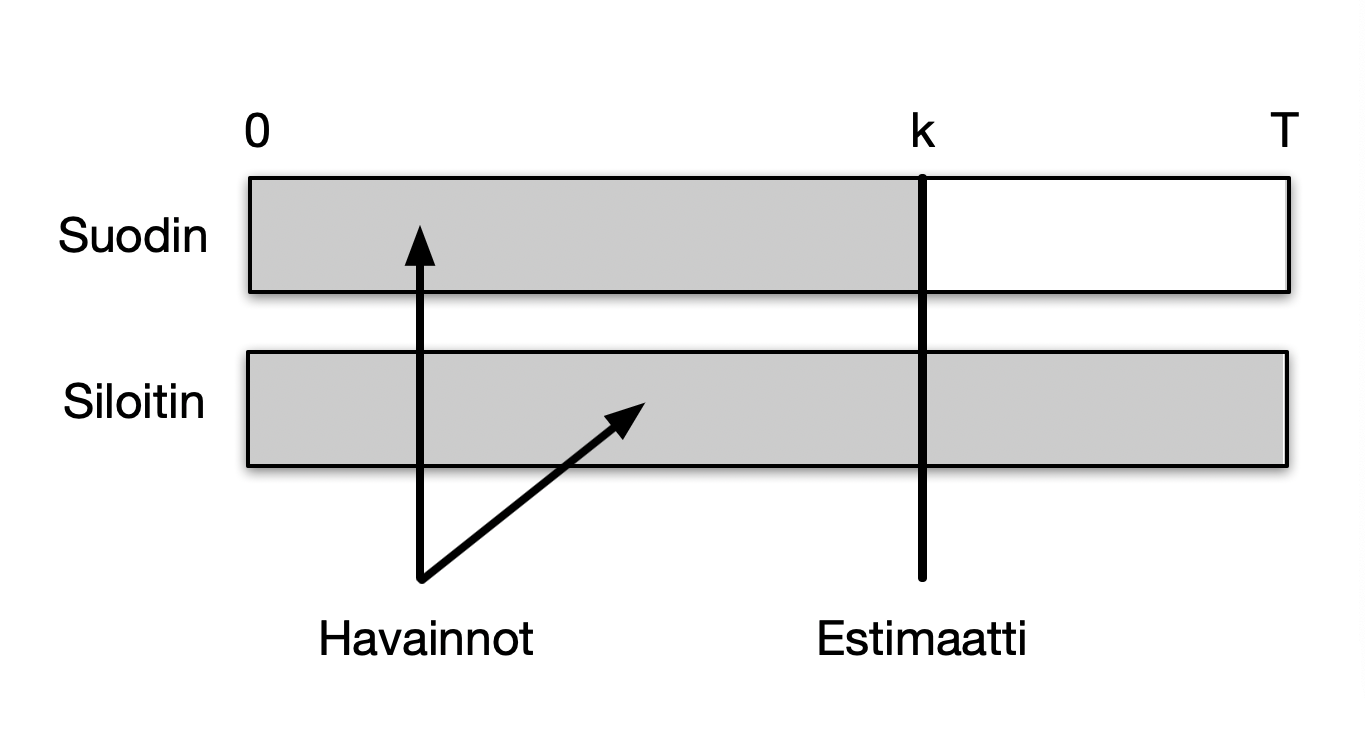
\includegraphics[width=9cm]{suodin_vs_siloitin_cropped}
\caption{Suodin- ja siloitteluongelma}
\label{fig:suodin_vs_siloitin}
\end{figure}

\section{Suodin- ja siloitteluongelmien historiaa}

Tämä alaluku esittää pääpiirteittään suodinongelmalle esitettyjen ratkaisujen historian. Lineaarisen suodinongelman osalta alaluku noudattaa Dan Crisanin artikkelia ``The stochastic filtering problem: a brief historical account'' (2014) \citep{crisan-2014} sekä Mohinder S. Grewalin ja Angus P. Andrewsin artikkelia ``Applications of Kalman Filtering in Aerospace 1960 to the Present'' (2010) \citep{Grewal-2010}. Hiukassuotimien osalta lähteenä toimii Cappé \&al (2007) \citep{cappe-2007}.

Suodinongelma nousi esille insinööritieteiden sekä sotateollisuuden käytännön ongelmista 2. maailmansodan aikana, vaikkakin suodinongelman diskreetin ajan ratkaisut juontavat jo Andrei N. Kolmogorovin 30-luvun artikkeleihin. Jatkuvan ajan tilanteessa ensimmäisen optimaalisen, kohinan sallivan suotimen esitti matemaatikko, kybernetiikan kehittäjä Norbert Wiener. Wiener-suotimena tunnettua ratkaisuaan varten Wiener muotoili seuraavat kolme ominaisuutta, jotka prosessin \(X_t\) estimaatin \(\hat{X}_t\) pitää toteuttaa.

\begin{enumerate}
\vspace{\baselineskip}
\item \textit{Kausaliteetti}: $X_t$ tulee estimoida käyttäen arvoja $Y_s$, missä $s \leq t$.
\item \textit{Optimaalisuus}: $X_t$:n estimaatin $\hat{X}_t$ tulee minimoida keskineliövirhe $\mathbb{E}[(X-\hat{X}_t)^2]$.
\item \textit{On-line-estimointi}: Estimaatin $\hat{X}_t$ tulee olla saatavissa minä hyvänsä ajanhetkenä $t$. 
\vspace{\baselineskip}
\end{enumerate}

Wiener sovelsi ratkaisussaan stationaaristen prosessien spektriteoriaa. Tulokset julkaistiin salaisina Yhdysvaltojen asevoimien tutkimuksesta vastanneen National Defense Research Committeen (NDRC) raportissa vuonna 1942. Tutkimus tunnettiin sodan aikana lempinimellä ``Keltainen vaara'' sekä painopaperinsa värin että vaikeaselkoisuutensa vuoksi. Myöhemmin Wiener esitti tuloksensa julkisesti kirjassaan \textit{Extrapolation, Interpolation and Smoothing of Stationary Time Series} (1949). Wienerin alkuperäiset kolme perusperiaatetta päteveät edelleen kaikille suodinongelman ratkaisuille, myös hiukassuotimille.

Kenties tärkein ja varmasti tunnetuin lineaariseen suodinongelman ratkaisu on Kalman-suodin. Suotimen kehittivät R.E. Kalman ja R.S. Bucy 1950- ja 60-lukujen taitteessa Yhdysvaltain kylmän sodan kilpavarustelutarpeisiin perustetussa Research Institute for Advanced Studies -tutkimuslaitoksessa (RIAS). Kalman-suodin on suodinongelman diskreetin ajan ratkaisu, kun taas Kalman-Bucy-suodin on jatkuvan ajan ratkaisu. Kohinan ollessa normaalijakautunutta on Kalman-suodin Wiener-suotimen tavoin lineaarisen suodinongelman optimaalinen ratkaisu. Wiener-suotimella ja Kalman-suotimella on kuitenkin erilaiset oletukset, minkä vuoksi erityisesti säätö- ja paikannussovelluksissa Kalman-suotimen käyttö on luontevampaa. Suotimien oletuksia ja oletusten välisiä eroja ei käsitellä tässä tutkielmassa, mutta alaluvussa \ref{kf-yhteydet-erot} käsitellään Kalman-suotimen formaalia yhteyttä hiukassuotimiin.

Kalman-suodinta voidaan soveltaa myös epälineaarisessa tapauksessa, kunhan suodinongelman funktiot \(f(\cdot)\) ja \(h(\cdot)\) ovat derivoituvia ja niihin liittyvä kohina oletetaan normaalijakautuneeksi. Tätä ratkaisua kutsutaan laajennetuksi Kalman-suotimeksi (extended Kalman filter, EKF). Suodin kehitettiin 60-luvulla NASA:n Apollo-ohjelman tarpeisiin, vaikkakin itse avaruusalusten laitteistot hyödynsivät lentoratojen laskennassa Kalman-suotimen perusversiota. Laajennetun Kalman-suotimen toimintaperiaate perustuu epälineaaristen funktioiden linearisointiin Taylorin kehitelmän avulla kulloisenkin estimaatin ympärillä. Laajennettu Kalman-suodin on erityisesti paikannussovellusten \textit{de facto} -suodinstandardi, mutta suodin ei kuitenkaan ole epälineaarisen ongelman optimaalinen estimaattori.

Kalman-suotimesta on lisäksi olemassa lukuisia muita epälineaarisiin ongelmiin soveltuvia laajennuksia, muun muassa paikkaratkaisun Kalman-suodin (\emph{position Kalman filter}, PKF), hajustamaton Kalman-suodin (\emph{unscented Kalman filter}, UKF) sekä tilastollisesti linearisoitu Kalman-suodin (\emph{statistically linearized Kalman filter}, SLF). Kuitenkin jos prosessin \(X_t\) mallia ei tunneta tarkasti tai kohinaa ei voida olettaa normaalijakautuneeksi, ovat hiukassuotimet eli sekventiaaliset Monte Carlo -menetelmät Kalman-suotimen johdannaisia parempia ratkaisuja. Vaikka tila-avaruuden dimensioiden kasvaessa kasvaa myös hiukassuotimien vaatima laskentateho, ovat hiukassuotimet aina sitä parempia mitä epälineaarisempia mallit ovat ja mitä kauempana normaalijakaumasta kohina on. Viimeisten vuosikymmenten aikana myös laskennan teho on kasvanut merkittävästi samalla kun laskennan hinta on vastaavasti romahtanut, mikä puoltaa Monte Carlo -menetelmien käyttöä entistä useammissa ongelmissa.

Joitakin suodinongelman rekursiivisia Monte Carlo -ratkaisuja löytyy jo 1950\textendash 70-luvuilta, erityisesti säätöteoriaan piiristä. Olennainen nykyalgoritmeihin periytynyt oivallus varhaisissa suodinalgoritmeissa oli tärkeytysotannan käyttö halutun jakaumaestimaatin laskennassa. Tärkeytysotanta-algoritmiin voidaan turvautua, kun emme pysty suoraan tekemään havaintoja jostakin jakaumasta \(p\) ja teemme sen sijaan havaintoja jakaumasta \(q\), jota painotamme niin, että tuloksena saadaan jakauman \(p\) harhaton estimaatti. Algoritmi on kuvattu tarkemmin tutkielman luvussa \ref{hiukassuotimet}.

Tärkeytysotantaa käyttävä suodinongelman ratkaiseva SIS-algoritmi (\emph{sequential importance sampling}) ei kuitenkaan vielä 70-luvulla löytänyt suurta käytännön suosiota. Osin tämä johtui puutteellisesta laskentatehosta, mutta algoritmi kärsi myös otosten ehtymisenä (\emph{sample impoverishment}) tunnetusta ongelmasta. Monissa ongelmissa SIS-algoritmia käytettäessä suuri osa painoista päätyy vain tietyille partikkeleille, jolloin vastaavasti suuri osa partikkeleista ei enää estimoi haluttua jakaumaa. Tähän ongelmaan palataan myöhemmin.

Merkittävän ratkaisun ehtymisongelmaan esittivät Gordon, Salmond ja Smith artikkelissaan ``Novel approach to nonlinear/non-Gaussian Bayesian state estimation'' (1993). \citep{Gordon-1993} Artikkelin ratkaisu kulki nimellä \emph{bootstrap filter}, saapasremmisuodin. Saapasremmisuodin vältti ehtymisen uudellenotannalla, jossa matalapainoiset partikkelit korvattiin otoksilla korkeapainoisemmista partikkeleista. Ratkaisussa painot eivät myöskään riippuneet partikkelien aiemmista poluista vaan ainoastaan havaintojen uskottavuusfunktiosta. Vastaavaa ratkaisua käytetään tämän tutkielman uudemmassa SIR-algoritmissa (\emph{sampling importance resampling}), jossa myös uudelleenotantaan sovelletaan tärkeytysotantaa.

Sekventiaalisissa Monte Carlo -menetelmissä stokastisen prosessin posteriorijakauman esittämiseen käytettyjä otoksia kutsutaan myös partikkeleiksi tai hiukkasiksi ja menetelmiä siten hiukassuotimiksi. Erityisesti myöhemmin esitettävää SIR-algoritmia kutsutaan usein hiukkassuotimeksi. Termiä hiukkassuodin käytti ensimmäisen kerran Del Moral artikkelissa ``Nonlinear Filtering: Interacting Particle Resolution'' (1996) \citep{DelMoral-1996}, SMC-menetelmät termiä Liu ja Chen artikkelissa ``Sequential Monte Carlo Methods for Dynamic Systems'' (1998) \citep{Liu-1998}. Tässä tutkielmassa käytetään yleisemmin käytettyä termiä hiukassuotimet.

\section{Monte Carlo -menetelmistä}

Tässä alaluvussa kuvataan lyhyesti hiukassuotimissa käytettävien Monte Carlo -menetelmien perusperiaate todennäköisyysjakauman estimoinnissa. Lisäksi esitetään tärkeytysotanta-algoritmi (\emph{importance sampling}), jonka tarkoituksena on estimoida harhattomasti jakaumaa \(p(x|y_{1:k})\), josta emme voi suoraan tehdä otoksia, mutta jota voimme approksimoida toisella jakaumalla \(q\). Esitykset noudattavat Särkkää (2013) \citep{sarkka-2013}.

\subsection{Monte Carlo -approksimaatio}

Bayesilaisessa päättelyssä ollaan yleisesti kiinnostuttu laskemaan johonkin posterioritiheysjakaumaan \(p\) liittyvää odotusarvoa

\begin{align}
\mathbb{E}[g(x)|y_{1:k}]=\int g(x)p(x|y_{1:k})dx,
\end{align}

\noindent missä \(g\) on tila-avaruuden mielivaltainen funktio ja \(p(x|y_{1:t})\) on havaintoihin \(\{y_1,\ldots,y_k\}\) liittyvä \(x\):n posterioritiheysjakauma. Odotusarvo on laskettavissa suljetussa muodossa vain harvoissa tapauksissa, suodinongelman kohdalla silloin, kun kyseessä on lineaarinen ja Gaussinen malli. Odotusarvoa voidaan kuitenkin approksimoida niin sanoituilla Monte Carlo -menetelmillä. Menetelmien perusperiaate on tehdä riippumattomia otoksia estimoitavasta jakaumasta ja laskea haluttu odotusarvo otosten avulla. Jos tehdään \(N\) otosta jakaumasta \(x^i\sim p(x|y_{1:t})\), missä \(i=\{1,\ldots,N\}\) saadaan näiden otosten avulla laskettua odotusarvon estimaatti

\begin{align}
\mathbb{E}[g(x)|y_{1:k}]\simeq\frac{1}{N}\sum_{i=1}^N g(x^i).
\end{align}

Monte Carlo -estimaatti konvergoi keskeisen raja-arvolauseen nojalla ja sen estimointivirheen voidaan osoittaa olevan luokkaa \(\mathcal{O}(\frac{1}{\sqrt{N}})\) riippumatta tilamuuttujan \(x\) dimensiosta. Hiukassuotimet hyödyntävät Monte Carlo -estimointia sekventiaalisesti, jolloin estimaatti lasketaan rekursiivisesti kullekin ajanhetkelle \(k=\{1,\ldots, t\}\). Tähän palataan luvuissa \ref{hiukkassiloittimet} ja \ref{paikannusesimerkki}.

\subsection{Tärkeytysotanta}

Tilanteessa, jossa Monte Carlo -otoksia ei voida tehdä suoraan jakaumasta \(p\), voidaan hyödyntää jakaumaa \(p\) approksimoivaa tärkeytys- tai ehdotusjakaumaa \(q(x|y_{1:k})\) sekä ns. tärkeytysotantaa. Oletetaan, että tunnetaan priorijakauma \(p(x)\) ja on olemassa havaintomalli \(p(y_{1:k}|x)\) sekä valittu ehdotusjakauma \(q(x|y_{1:k})\), josta voidaan tehdä otoksia. Ehdotusjakaumalta edellytetään lisäksi, että sen kantaja on suurempi tai yhtä suuri kuin jakauman \(p(x|y_{1:k})\) ja että se saa nollasta poikkeavia arvoja kaikkialla missä \(p(x|y_{1:k})\) saa nollasta poikkeavia arvoja. Kirjoitetaan halutun posteriorijakauman odotusarvo integraalina

\begin{align}
\int g(x)p(x|y_{1:k})dx=\int g(x)\frac{p(x|y_{1:k})}{q(x|y_{1:k})}q(x|y_{1:k})dx,
\end{align}

\noindent jolle voidaan muodostaa Monte Carlo -approksimaatio tekemällä \(N\) otosta jakaumasta \(x^i \sim q(x|y_{1:k})\).

Muodostetaan näin odotusarvo

\begin{align}
\mathbb{E}[g(x)|y_{1:k}]\simeq\frac{1}{N}\sum_{i=1}^N\frac{p(x^i|y_{1:k})}{q(x^i|y_{1:k})}g(x^i)=\sum_{i=1}^Nw^ig(x^i),
\end{align}

\noindent missä \(g(x)\) on jokin estimoinnissa hyödyllinen, mielivaltainen funktio. Tutkielmassa käytetty notaatio \(x_k^i\) viittaa ajanhetken \(k\) partikkeliin \(i\), missä \(i=\{1,\ldots,N\}\). Tärkeytysotantaa kuvaa nyt algoritmi (\ref{tarkeytysotanta-algo}). Kun posteriorijakauman estimaatti muodostetaan kyseisellä algoritmilla voidaan tulos kirjoittaa

\begin{align}
\hat{p}(x|y_{1:k})=\sum_{i=1}^{N}w^i \delta(x-x^i),
\end{align}

\noindent missä \(\delta(x)\) on Diracin deltafunktio.

\begin{algorithm}[H]
\label{tarkeytysotanta-algo}
\DontPrintSemicolon
\Begin{
  \For{$i=1,2,\ldots,N$}{
    \Begin{Otetaan $N$ otosta ehdotusjakaumasta $x^i \sim q(x|y_{1:k}).$}
    \Begin{Lasketaan normalisoimattomat painot $w_*^i= p(y_{1:k}|x^i)p(x^i)/q(x^i|y_{1:k}).$ \newline ja normalisoidut painot $w^i=w_*^i/\sum_{j=1}^Nw_*^j$.}
    \Begin{Estimoidaan $p$ laskemalla tiheydelle approksimaatio $\mathbb{E}[g(x)|y_{1:k}]\simeq\sum_{i=1}^Nw^ig(x^i)$.}
    } 
  }  
\caption{Tärkeytysotanta}
\end{algorithm}

\section{Bayesilainen suodin} \label{bayesilainen-suodin}

Suodinongelmassa ollaan kiinnostuttu tilavektorin posteriorijakauman \(p(x_k|y_{1:k})\) estimoinnista. Tässä alaluvussa käydään läpi yleinen rekursiivinen, Bayesilainen posteriorijakauman laskenta. Tällaista suodinongelman ratkaisua kutsutaan myös Bayesilaiseksi suotimeksi. Koska epälineaarisessa, ei-normaalijakautuneessa tilanteessa rekursiota ei voida laskea analyyttisesti, pitää estimoinnissa käyttää numeerisia menetelmiä. SMC-menetelmissä tämä tarkoittaa jakauman sekventiaalista Monte Carlo -approksimointia, jonka toteutus esitetään alaluvun \ref{paikannusesimerkki} algoritmissa. Molemmat esitykset noudattavat Gustafssonia (2010).

Bayesilainen ratkaisu tilavektorin posteriorijakauman estimaatille \(\hat{p}(x_k|y_{1:k})\) saadaan seuraavalla rekursiolla (käydään läpi jokaiselle ajanhetkelle \(k=\{1,\ldots,t\}\)). Lasketaan ensin

\begin{align}\label{bayes-paivitys}
p(x_k|y_{1:k}) = \frac{p(y_k|x_k)p(x_k|y_{1:k-1})}{p(y_k|y_{1:k-1})},
\end{align}

\noindent joka saadaan suoraan Bayesin kaavasta \(P(A|B)=P(B|A)P(A)/P(B)\). Normalisointivakio lasketaan integraalina

\begin{align}\label{bayes-normalisointi}
p(y_k|y_{1:k-1})=\int_{\mathbb{R}^{n_x}}p(y_k|x_k)p(x_k|y_{1:k-1})\mathop{dx_k},
\end{align}

\noindent joka saadaan kokonaistodennäköisyyskaavasta \(P(A)=\mathbb{E}[P(A|X)]=\int_{-\infty}^{\infty}P(A|X=x)f_X(x)\mathop{dx}\). Merkintä \(\mathbb{R}^{n_x}\) vastaa tässä piilossa olevan tilavektorin dimensiota \(n\).

Lopuksi lasketaan päivitysaskel ajalle, joka saadaan edelleen kokonaistodennäköisyydellä

\begin{align}\label{bayes-aikapaivitys}
p(x_{k+1}|y_{1:k})=\int_{\mathbb{R}^{n_x}}p(x_{k+1}|x_k)p(x_k|y_{1:k})\mathop{dx_k}.
\end{align}

\noindent Rekursion avulla voimme laskea jakauman \(p(x_k|y_{1:k})\) estimaatti käymällä rekursion läpi \(k\) kertaa.

\section{Kalman-suotimen ja hiukassuotimen yhteydestä ja eroista} \label{kf-yhteydet-erot}

Tässä alaluvussa käsitellään lyhyesti Kalman-suotimen yhteyttä hiukassuotimeen edellä estitetyn teorian valossa. Esitys noudattaa Särkkää (2013). \citep{sarkka-2013} Merkitään kuten edellä dynaamista mallia \(x_k\) ja havaintomallia \(y_k\) ja oletataan toisin kuin edellä, että nämä ovat lineaarisia ja noudattavat normaalijakaumaa. Koska mallit ovat lineaarisia, voidaan ne nyt kirjoittaa muotoon

\begin{align}
&\label{kalman-malli1}x_k=\mathbf{A}_{k-1}x_{k-1}+q_{k-1},\\
&\label{kalman-malli2}y_k=\mathbf{H}_k x_k + r_k
\end{align}

missä \(\mathbf{A}_{k-1}\) on dynaamisen mallin tilasiirtymään kuvaava matriisi ja \(\mathbf{H}_k\) on havaintojen mallimatriisi. Normaalisuusoletuksesta puolestaan seuraa, että sekä mallin että prosessin kohinavektorit noudattavat normaalijakaumia \(q_{k-1} \sim \mathbb{N}(0, \mathbf{Q}_{k-1})\) ja \(r_k \sim \mathbb{N}(0, \mathbf{R}_k)\), missä \(\mathbf{Q}_{k-1}\) ja \(\mathbf{R}_k\) ovat kovarianssimatrsiiseja. Lisäksi oletetaan, että prosessin priorijakauma on normaali eli \(x_0 \sim \mathbb{N}(m_0, \mathbf{P_0})\). Mallit voidaan nyt kirjoittaa tiheysfunktiomuodossa

\begin{align}
&\label{kalman-malli-pdf1}p(x_k|x_{k-1})=\mathcal{N}(x_k|\mathbf{A}_{k-1}x_{k-1},\mathbf{Q}_{k-1})\\
&\label{kalman-malli-pdf2}p(y_k|x_k)=\mathcal{N}(y_k|\mathbf{H}_{k}x_{k},\mathbf{R}_{k}),
\end{align}

joista voidaan edelleen johtaa suodinongelman mallit

\begin{align}
&\label{kalman-malli-suodin1}p(x_k|y_{1:k-1})=\mathcal{N}(x_k|m_k^* ,\mathbf{P}_k^*)\\
&\label{kalman-malli-suodin2}p(x_k|y_{1:k})=\mathcal{N}(x_k|m_k ,\mathbf{P}_k)\\
&\label{kalman-malli-suodin3}p(y_k|y_{1:k-1})=\mathcal{N}(y_k|\mathbf{H}_k m_k^* ,\mathbf{S}_k)
\end{align}

ja ongelma ratkaista näin algoritmilla \(\ref{kf}\).

\begin{algorithm}[H]
\label{kf}
\DontPrintSemicolon
\SetAlgoShortEnd
\KwResult{Posteriorijakauman $p(x_{1:k}|y_{1:k})$ estimaatti.\;}
\KwData{Havainnot $y_k$. Priorijakauman $x_0$ keskiarvovektori $m_0$ ja kovarianssimatriisi $\mathbf{P}_0$.\;}
\Begin{
  \For{$k=\{1,2,\ldots,t\}$}{
    \Begin{Ennusteaskel. \newline $m_k^*= \mathbf{A}_{k-1}m_{k-1}$\;}
    \If{$k < t$}{\Begin{Päivitysaskel. \newline $v_k = y_k - \mathbf{H}_k m_k^*$
    \newline $\mathbf{S}_k = \mathbf{H}_k \mathbf{P}_k^* \mathbf{H}_k^\top + \mathbf{R}_k$
    \newline\ $\mathbf{K}_k = \mathbf{P}_k^* \mathbf{H}_k^\top \mathbf{S}_k^{-1}$
    \newline\ $m_k = m_k^* \mathbf{K}_k v_k$
    \newline\ $\mathbf{P}_k = \mathbf{P}_k^* - \mathbf{K}_k \mathbf{S}_k \mathbf{K}_k^\top$;}}
  }  
}
\caption{Kalman-suodin}
\end{algorithm}

Esitetty algoritmi on ns. Kalman-suodin, joka selkeästi toimii suodinongelman ratkaisuna, kun mallit ovat haluttua lineaarista normaalimuotoa. Jos tämä oletus ei täyty, on Kalman-suotimesta kehitetty useita versioita, joissa ei-lineaarinen malli voidaan linearisoida tiettyjen ehtojen vallitessa.

Tämän alaluvun tarkoituksena oli esittää, että Kalman-suotimessa ongelma on samaa muotoa kuin hiukassuotimessa, joten linearisoituja Kalman-suotimia ei tässä käsitellä. Hiukassuodin myös ratkaisee ongelman mille hyvänsä epälineaariselle mallille.

\chapter{Hiukassuotimet} \label{hiukassuotimet}

\section{SIR-algoritmi}

Tässä alaluvussa esitetään SMC-menetelmiin kuuluva SIR-algoritmi, epälineaarisen suodinongelman ratkaisemiseksi. Algoritmi on numeerinen toteutus luvussa \ref{bayesilainen-suodin} kuvatusta Bayesilaisesta suotimesta. Esitetty algoritmi perustuu Gustafssoniin (2010). Ilman uudelleenotantavaihetta kyseessä olisi SIS-algoritmi.

Algoritmi alustetaan jakaumasta \(x_1^i\sim p_{x_0}\) generoiduilla \(N\) kappaleella partikkeleita. Jokaiselle partikkelille annetaan alustuksessa sama paino \(w_{1|0}^i=1/N\). Algoritmi suoritetaan jokaiselle partikkelille \(i=\{1,2,\ldots,N\}\) jokaisella ajanhetkellä \(k=\{1,2,\ldots,t\}\).

Seuraava toistetaan jokaiselle ajanhetkelle \(k=\{1,2,\ldots,t\}\). Algoritmin ensimmäisessä vaiheessa päivitetään painot yhtälön (\ref{painopaivitys}) mukaan.

\begin{align}\label{painopaivitys}
w^i_{k|k}=\frac{1}{c_k}w^i_{k|k-1}p(y_k|x^i_k).
\end{align}

\noindent Tämä vastaa yllä esitetyn Bayes-suotimen päivitysvaihetta (\ref{bayes-paivitys}). Normalisointipaino \(c_k\) lasketaan puolestaan yhtälöstä (\ref{normalisointi}), mikä vastaa Bayes-suotimen normalisointivakion laskemista (\ref{bayes-normalisointi}) ja asettaa painojen summaksi \(\sum_{i=1}^Nw^i_{k|k}=1\).

\begin{align}\label{normalisointi}
c_k=\sum_{i=1}^{N}w_{k|{k-1}}^ip(y_k|x_k^i).
\end{align}

\noindent Seuraavassa vaiheessa estimoidaan \(p\) laskemalla tiheyden \(p(x_{1:k}|y_{1:k})\) Monte Carlo -estimaatti yhtälön (\ref{p-estimaatti}) perusteella

\begin{align}\label{p-estimaatti}
\hat{p}(x_{1:k}|y_{1:k})=\sum_{i=1}^{N}w_{k|k}^i \delta(x_{1:k}-x_{1:k}^i).
\end{align}

Tämän jälkeen suoritetaan valinnainen uudelleenotanta. Uudelleenotanta voidaan tehdä jokaisella askeleella tai efektiivisen otoskoon perusteella alla kuvatun kynnysarvoehdon \(\hat{N}_{eff}< N_{th}\) täyttessä, jolloin uudelleenotantaa kutsutaan adaptiiviseksi uudelleenotannaksi. Tällaista uudelleenotantaa hyödynnetään esitetyssä algoritmissa (\ref{sir}). Lopuksi päivitetään aika (jos \(k < t\)), luodaan uudet ennusteet partikkeleille ehdotusjakaumasta (\ref{ehdotusjakauma})

\begin{align}\label{ehdotusjakauma}
x_{k+1}^i\sim q(x_{k+1}|x_k^i,y_{k+1})
\end{align}

\noindent ja päivitetään partikkelien painot tärkeytysotannalla (\ref{tarkeytys}), sen mukaan kuinka todennäköisiä partikkelien ennusteet ovat

\begin{align}\label{tarkeytys} w_{k+1|k}^i=w_{k|k}^i\frac{p(x_{k+1}^i|x_k^i)}{q(x_{k+1}^i|x_k^i,y_{k+1})}.
\end{align}

\noindent Vaiheet \ref{ehdotusjakauma} ja \ref{tarkeytys} vastaavat Bayes-suotimen aikapäivitystä (\ref{bayes-aikapaivitys}).

Alla käsitellään algoritmiin liittyvän uudelleenotantamenetelmän, partikkelien määrän ja ehdotusjakauman valinta. Lopuksi esiteetään algoritmin konvergenssia, marginaalijakaumaa sekä aikakompleksisuutta koskevia tuloksia.

\begin{algorithm}[H]
\label{sir}
\DontPrintSemicolon
\SetAlgoShortEnd
\KwResult{Posteriorijakauman $p(x_{1:k}|y_{1:k})$ estimaatti.\;}
\KwData{Havainnot $y_k$. Generoitu $x_1^i\sim p_{x_0}$ missä $i=\{1,\ldots,N\}$ ja jokainen partikkeli saa saman painon $w_{1|0}^i=1/N$.\;}
\Begin{
  \For{$k=\{1,2,\ldots,T\}$}{
    \For{$i=\{1,2,\ldots,N\}$}{
      \Begin{Päivitetään painot $w_{k|k}.$\;}
      \Begin{Estimoidaan $p$ laskemalla tiheydelle approksimaatio $\hat{p}(x_{1:k}|y_{1:k})=\sum_{i=1}^{N}w_{k|k}^i \delta(x_{1:k}-x_{1:k}^i)$.\;}
    }
    \Begin{Lasketaan efektiivinen otoskoko $\hat{N}_{eff}$.\;}
    \If{$\hat{N}_{eff}< N_{th}$}{\Begin{Otetaan uudet $N$ otosta palauttaen joukosta $\{x_{1:k}^i\}_{i=1}^N$, missä otoksen $i$ todennäköisyys on $w^i_{k|k}$.\;}
    \Begin{Asetetaan painot $w^i_{k|k}=1/N$.\;}}
    \If{$k < T$}{\Begin{Aikapäivitys. \newline Luodaan ennusteet partikkeleille ehdotusjakaumasta $x_{k+1}^i\sim q(x_{k+1}|x_k^i,y_{k+1})$, \newline päivitetään partikkelien painot tärkeytysotannalla.\;}}
  }  
}
\caption{SIR}
\end{algorithm}

\subsection{Parametrien valinta}

Ennen algoritmin suorittamista valitaan ehdotusjakauma \(q(x_{k+1}|x_{1:k},y_{k+1})\), uudelleenotantamenetelmä sekä partikkelien määrä \(N\). Ehdotusjakauman ja uudelleenotantamenetelmän valinnassa tärkeimpänä päämääränä on välttää otosten ehtymistä, kun taas partikkelien määrä säätelee kompromissia algoritmin suorituskyvyn ja tarkkuuden välillä.

\subsubsection{Otoskoon $N$ valinta}

Yleispätevää sääntöä otoskoon/partikkelien lukumäärän \(N\) valinnalle on vaikeaa antaa, sillä vaadittava estimointitarkkuus riippuu usein käsillä olevasta ongelmasta. Gordon \&al.~(1993) esittävät kuitenkin kolme tekijää, jotka vaikuttavat partikkelien lukumäärän valintaan

\begin{enumerate}
\def\labelenumi{\alph{enumi}.}
\tightlist
\item
  tila-avaruuden ulottuvuuksien lukumäärä \({n_x}\),
\item
  tyypillinen päällekäisyys priorin ja uskottavuuden välillä
\item
  sekä tarvittava aika-askelten lukumäärä.
\end{enumerate}

Ensimmäisen tekijän vaikutus on selvä. Mitä useammassa ulottuvuudessa otantaa tarvitsee tehdä, sen korkeammaksi on \(N\) asetettava, jotta jokainen ulottuvuus pystytään kattamaan. Tekijät (\textit{b}) ja (\textit{c}) puolestaan seuraavat uudelleenotannasta. Jos se osa tila-avaruutta, jossa uskottavuus \(p(y_k|x_k)\) saa merkittäviä arvoja on pieni verrattuna siihen osaan, jossa priorijakauma \(p(x_k|y_{1:k-1})\) saa merkittäviä arvoja, suuri osa partikkeleista saa pieniä painoja eikä näin valikoidu uudelleenotantaan.

Yleisesti ottaen \(N\) kannattaa asettaa sellaiseksi, että se paitsi tuottaa riittävän tarkan estimaatin, on se käytettävissä olevan laskentatehon sekä vaadittavan laskentanopeuden kannalta järkevää. Tähän palataan tutkielman lopuksi empiirisessä paikannusesimerkissä.

\subsubsection{Uudelleenotantamenetelmän valinta}

Ilman uudelleenotantaa on mahdollista, että algoritmi alkaa kärsiä SIS-algoritmille ominaisesta otosten ehtymisestä. Toisin sanoen kaikki painot alkavat keskittyä vain muutamalle partikkelille eikä algoritmi enää approksimoi tehokkaasti haluttua jakaumaa. Uudelleenotanta tarjoaa osittaisen ratkaisun tähän ongelmaan, mutta hävittää samalla informaatiota ja siten lisää satunnaisotantaan liittyvää epävarmuutta. Yleisesti ottaen uudelleenotanta kannattaa aloittaa vasta siinä vaiheessa algoritmin suorittamista, kun siitä on otosten ehtymisen kannalta hyötyä, esimerkiksi efektiivisen otoskoon pudottua jonkin kynnysarvon alapuolelle (adaptiivinen uudelleenotanta). Efektiivinen otoskoko saadaan laskettua variaatiokertoimesta \(c_\nu\) kaavalla

\begin{align}\label{N-eff}
N_{eff}= \frac{N}{1+c_\nu^2(w^i_{k|k})} = \frac{N}{1+\frac{\text{Var}(w^i_{k|k})}{(\mathbb{E}[w^i_{k|k}])^2}} =\frac{N}{1+N^2\text{Var}(w^i_{k|k})}.
\end{align}

Näin laskettu efektiivinen otoskoko maksimoituu (\(N_{eff}=N\)), kun kaikille painoille pätee \(w^i_{k|k}=1/N\) ja minimoituu (\(N_{eff}=1\)), kun \(w^i_{k|k}=1\) todennäköisyydellä \(1/N\) ja \(w^i_{k|k}=0\) todennäköisyydellä \((N-1)/N\). Normalisoitujen painojen avulla saadaan effektiiviselle otoskoolle ajanhetkellä \(k\) laskennallinen approksimaatio

\begin{align}\label{N-hat-eff}
\hat{N}_{eff}=\frac{1}{\sum_{i=1}^N(w^i_{k|k})^2}.
\end{align}

Sekä määritelmälle (\(\ref{N-eff}\)) että (\(\ref{N-hat-eff}\)) pätee \(1 \leq \hat{N}_{eff} \leq N\). Yläraja saavutetaan, kun jokaisen partikkelin paino on sama. Alarajalle päädytään, kun kaikki paino keskittyy yksittäiselle partikkelille. Tästä saadaan määriteltyä algoritmille SIR-uudelleenotantaehto \(\hat{N}_{eff}< N_{th}\). Gustafsson (2010) \citep{gustafsson-2010} esittää uudelleenotannan kynnysarvoksi esimerkiksi \(\hat{N}_{th}=2N/3\).

Uudelleenotanta ei muuta approksimoitavan jakauma \(p\) odotusarvoa, mutta se lisää jakauman Monte Carlo -varianssia. On kuitenkin olemassa esimerkiksi osittamiseen perustuvia uudelleenotantamenetelmiä, jotka pyrkivät minimoimaan varianssin lisäyksen. Varianssin pienennysmenetelmät jätetään tämän tutkielman ulkopuolelle.

\subsubsection{Ehdotusjakauman valinta}

Yksinkertaisin muoto ehdotusjakaumalle on \(q(x_{1:k}|y_{1:k})\) eli jokaisella algoritmin suorituskerralla käydään läpi koko aikapolku \(1\):\(k\). Tämä ei kuitenkaan ole tarkoituksenmukaista, erityisesti jos kyseessä on reaaliaikainen sovellutus. Kirjoitetaan ehdotusjakauma muodossa

\begin{align}\label{proposal-factorization}
q(x_{1:k}|y_{1:k})=q(x_k|x_{1:k-1},y_{1:k})q(x_{1:k-1}|y_{1:k}).
\end{align}

Jos yhtälöstä (\ref{proposal-factorization}) poimitaan ehdotusjakaumaksi ainoastaan termi \(q(x_k|x_{1:k-1},y_{1:k})\) voidaan tämä kirjoittaa edelleen Markov-ominaisuuden nojalla muotoon \(q(x_k|x_{k-1},y_{k})\). Tämä on suodinongelman kannalta riittävää, koska olemme kiinnostuneita posteriorijakaumasta ja arvosta \(x\) ainoastaan ajanhetkellä \(k\) (tasoitusongelmassa tarvitsisimme koko polun \(x_{1:k}\)). Alla tarkastellaan edelleen Gustafssonia (2010) \citep{gustafsson-2010} seuraten kahta ehdotusjakauman valintatapaa, prioriotantaa (\emph{prior sampling}) sekä uskottavuusotantaa (\emph{likelihood sampling}).

Ennen ehdotusjakauman tarkastelua määritellään mallille signaali-kohinasuhde uskottavuuden maksimin ja priorin maksimin välisenä suhteena

\begin{align}\label{SNR}
\text{SNR}\propto \frac{\text{max}_{x_k}p(y_k|x_k)}{\text{max}_{x_k}p(x_k|x_{k-1})}. 
\end{align}

\noindent Yhdistetään lisäksi ehdotusjakaumia varten yhtälöt (\ref{painopaivitys}) ja (\ref{normalisointi}), jolloin saadaan painojen päivitys muotoon

\begin{align}\label{painopaivitys-propto}
w^i_{k|k} \propto w^i_{k-1|k-1}\frac{p(y_k|x^i_k)p(x_k|x^{k-1})}{q(x_k|x^i_{k-1},y_k)}.
\end{align}

Kun suhde (\ref{SNR}) on matala, on prioriotanta luonnollinen valinta. Tässä käytetään ehdotusjakaumana tilavektorin ehdollista prioria eli

\begin{align}\label{prioriotanta-q}
q(x_k|x_{1:k-1},y_{k})=p(x_k|x^i_{k-1}).
\end{align}

\noindent Yhtälön (\ref{prioriotanta-q}) perusteella saadaan edelleen prioriotannan painoiksi

\begin{align}\label{prioriotanta-w}
w^i_{k|k} = w^i_{k|k-1}p(y_k|x^i_k) = w^i_{k-1|k-1}p(y_k|x^i_k).
\end{align}

Kun signaali-kohinasuhde on kohtalainen tai korkea, on parempi käyttää ehdotusjakaumana skaalattua uskottavuusfunktiota (\ref{uskottavuusotanta-q}). Tarkastellaan ensin tekijöihin jakoa

\begin{align}\label{uskottavuusotanta-factorization}
p(x_k|x^i_{k-1},y_k)=p(y_k|x_k)\frac{p(x_k|x^i_{k-1})}{p(y_k|x^i_{k-1})}.
\end{align}

\noindent Kun SNR on korkea ja uskottavuusfunktio on integroituva pätee \(p(x_k|x^i_{k-1},y_{k}) \propto p(y_k|x_k)\), jolloin voidaan asettaa (\ref{uskottavuusotanta-q})

\begin{align}\label{uskottavuusotanta-q}
q(x_k|x^i_{k-1},y_{k}) \propto p(y_k|x_k).
\end{align}

\noindent Yhtälön (\ref{uskottavuusotanta-q}) perusteella saadaan edelleen uskottavuusotannan painoiksi (\ref{uskottavuusotanta-w}).

\begin{align}\label{uskottavuusotanta-w}
w^i_{k|k} = w^i_{k-1|k-1}p(x^i_k|x^i_{k-1}).
\end{align}

\subsection{Konvergenssituloksia}

Alla esitetään kaksi SIR-algoritmiin liittyvää konvergenssitulosta. Se, kuinka hyvin esitetyllä algoritmilla arvioitu posterioritiheys \(\hat{p}(x_{1:k}|y_{1:k})\) approksimoi todellista tiheysfunktiota \(p(x_{1:k}|y_{1:k})\) sekä mikä on approksimaation keskineliövirhe. Tulokset 1\textendash 2 noudattavat Crisanin ja Doucet'n artikkeleita ``Convergence of Sequential Monte Carlo Methods'' (2000) \citep{crisan-2000} ja ``A Survey of Convergence Results on Particle Filtering Methods for Practitioners'' (2002) \citep{crisan-2002}, tulos 3 Chopinin artikkelia ``Central limit theorem for sequential Monte Carlo methods and its application to Bayesian inference'' (2004) \citep{chopin-2004}.

\textit{Konvergenssitulos 1}: Kun \(N \to \infty\) algoritmille pätee \(\forall k\) tulos (\ref{jakaumakonvergenssi}).

\begin{align}\label{jakaumakonvergenssi}
\hat{p}(x_{1:k}|y_{1:k}) \xrightarrow{a.s.} p(x_{1:k}|y_{1:k}).
\end{align}

\textit{Konvergenssitulos 2}: Keskineliövirheelle pätee asymptoottinen konvergenssi (\ref{MSE-konvergenssi}).

\begin{align}\label{MSE-konvergenssi}
\mathbb{E}(\hat{g}(x_k)-\mathbb{E}(g(x_k)))^2\leq\frac{p_k\norm{g(x_k)}}{N},
\end{align}

\noindent missä \(g\) on mikä hyvänsä piilossa olevan tila-avaruuden rajoitettu Borel-mitallinen funktio (\(g \in \mathcal{B}(\mathbb{R}^{n_x})\)), \(\norm{g(\cdot)}\) kyseisen funktion supremum-normi ja \(p_k\) jokin äärellinen vakio, jolle pätee ajanhetkestä \(k\) riippumatta \(p_k=p<\infty\).

\textit{Konvergenssitulos 3}: Keskeinen raja-arvolause (\ref{CLT}).

\begin{align}\label{CLT}
\text{Kun } N \to \infty: \sqrt{N} \left\{ \frac{1}{N} \sum_{i=1}^N \hat{g}(x_k^i) -\mathbb{E}(g(x_k^i)) \right\} \xrightarrow{D} \mathbb{N}(0,\sigma^2 < \infty),
\end{align}

missä \(g\) on jälleen mikä hyvänsä piilossa olevan tila-avaruuden rajoitettu Borel-mitallinen funktio (\(g \in \mathcal{B}(\mathbb{R}^{n_x})\)). Konvergenssituloksia ei tämän tutkielman puitteissa todisteta.

\subsection{Marginaalijakauma}

Edellä kuvattu algoritmi \ref{sir} tuottaa approksimaation koko prosessin posteriorijakaumalle \(p(x_{1:k}|y_{1:k})\). Jos halutaan tietää ainoastaan posteriorijakauman \(p(x_k|y_{1:k})\) estimaatti, voidaan käyttää yksinkertaisesti viimeisestä tilasta \(x_k\) laskettua estimaattia

\begin{align}
\hat{p}(x_{k}|y_{1:k})=\sum_{i=1}^{N}w_{k|k}^i \delta(x_{k}-x_{k}^i).
\end{align}

Toinen, tarkempi vaihtoehto on käyttää laskennassa tärkeytyspainoa

\begin{align}\label{marginaalitarkeytys}
w_{k+1|k}^i=\frac{\sum_{j=1}^{N}w_{k|k}^jp(x_{k+1}^i|x_k^j)}{q(x_{k+1}^i|x_k^i,y_{k+1})}
\end{align}

\noindent painon (\ref{tarkeytys}) sijaan. Tällöin jokaisella aikapäivitysaskeleella lasketaan painot kaikkien mahdollisten tila-aika-avaruuspolkujen yli. Samoin kuin uudelleenotanta tämä pienentää painojen varianssia.

\subsection{Aikakompleksisuus}

Algoritmin perusmuodon aikakompleksisuus on \(\mathcal{O}(N)\). Uudelleenotantamenetelmän tai ehdotusjakauman valinta ei suoraan vaikuta aikakompleksisuuteen. Sen sijaan marginalisointi tärkeytyspainolla (\ref{marginaalitarkeytys}) lisää algoritmin aikakompleksisuutta \(\mathcal{O}(N)\rightarrow\mathcal{O}(N^2)\), koska jokaisen partikkelin kohdalla painot lasketaan jokaisen tila-aika-avaruuspolun yli. On selvää, että erityisesti isoilla otoskoon \(N\) arvoilla ei yllä esitetty marginalisointi enää ole mielekästä.

Tällaisia tilanteita varten algoritmista on olemassa \(\mathcal{O}(N\text{log}(N))\) -versioita, jotka perustuvat esimerkiksi N:n kappaleen oppimiseen (\emph{N-body learning}). Näiden algoritmien käsittely jää tämän tutkielman ulkopuolelle, mutta katsauksen algoritmeista ovat esittäneet esimerkiksi Klaas \&al.~artikkelissa ``Toward Practical \(N^2\) Monte Carlo: the Marginal Particle Filter'' (2012).

\section{Saapasremmisuodin}

Saapasremmisuodin \ref{saapasremmisuodin} eli \emph{bootstrap filter} on SIR-algoritmin muunnelma, jossa tärkeytysotannan (kts. \ref{tarkeytysotanta-algo}) käytetään dynaamista mallia \(p(x_k|x_{k-1})\).

\begin{algorithm}[H]
\label{saapasremmisuodin}
\DontPrintSemicolon
\SetAlgoShortEnd
\KwResult{Posteriorijakauman $p(x_{1:k}|y_{1:k})$ estimaatti.\;}
\KwData{Havainnot $y_k$. Generoitu $x_1^i\sim p_{x_0}$ missä $i=\{1,\ldots,N\}$ ja jokainen partikkeli saa saman painon $w_{1|0}^i=1/N$.\;}
\Begin{
  \For{$k=\{1,2,\ldots,t\}$}{
    \For{$i=\{1,2,\ldots,N\}$}{
      \Begin{Luodaan uudet estimaatit dynaamisesta mallista $x_{k}^i\sim p(x_{k}|x_{k-1}^i)$.;}
      \Begin{Päivitetään hiukkasten painot $w_k^i$ uskottavuusfunktion $p(y_k|x_k^i)$ mukaan.}
      \Begin{Estimoidaan $p$ laskemalla tiheydelle approksimaatio $\hat{p}(x_{1:k}|y_{1:k})=\sum_{i=1}^{N}w_{k|k}^i \delta(x_{1:k}-x_{1:k}^i)$.}
    }
    \If{$k < t$}{\Begin{Aikapäivitys. Suoritetaan uudelleenotanta kuten SIR-algoritmissa \ref{sir}.\;}}
  }  
}
\caption{Saapasremmisuodin}
\end{algorithm}

Saapasremmisuodin on edellä esitettyä SIR-algoritmia yksinkertaisempi toteuttaa, mutta epäinformatiivisen tärkeytysjakauman vuoksi algoritmi saattaa vaatia SIR-algoritmia suuremman määrän hiukkasia. Saapasremmisuodin esitetään tässä sen historiallisen tärkeyden vuoksi, sillä kyseessä oli ensimmäinen uudelleenotataantaa hyödyntävä hiukassuodinalgoritmi. Suotimen käytännön toteutukseen palataan luvussa \ref{paikannusesimerkki}.

\section{Varianssin estimoinnista} \label{varianssin-estimointi}

Hiukassuotimen varianssin estimoinnissa ollaan kiinnostuneita jakaumaestimaatin \(\hat{p}(x_{1:k}|y_{1:k})\) varianssin estimoinnista. Yksinkertaisin tapa estimoida hiukassuodinalgoritmin varianssia on ajaa algoritmi \(M > 1\) kertaa. Koska ajot ovat toisistaan riippumattomia, voidaan estimaatin varianssi laskea kullekin ajanhetkelle \(k\) näiden ajojen \(k\)-hetken estimaattien otosvarianssina:

\begin{align}\label{MC-varianssi}
\hat{\sigma}^2_{MC} = \text{Var}_{\text{MC}}(\hat{p}(x_{1:k}|y_{1:k})) = \frac{1}{M-1} \sum_{i=1}^{M}(x_k^i-\bar{x_k})^2.
,\end{align}

missä \(x_k^i\) on \(k\):nen ajanhetken piste-estimaatti ajolle \(i=1,\ldots,M\) ja \(\bar{x_k}\) piste-estimaattien aritmeettinen keskiarvo laskettuna kaikkien \(M\) ajojen yli. Tällaisen Monte Carlo -varianssin estimoiminen on kuitenkin laskennallisesti tehotonta. Monissa käytännön sovelluksissa jo yhden hiukassuodinalgoritmin ajaminen vaatii runsaasti laskentatehoa, jolloin Monte Carlo -varianssin laskeminen ei ole mahdollista. Varianssia ei voi myöskään laskea analyyttisesti, mutta koska keskeisen raja-arvolauseen \ref{CLT} nojalla tiedetään, että asymptoottinen varianssi

\begin{align}\label{asymptoottinen-varianssi}
\lim_{N\to \infty} N \text {Var}(\hat{g}(x_k^i))
,\end{align}

on olemassa, on sen estimointiin kehitetty lähivuosina joitakin menetelmiä. Alla käsitellään Leen ja Whitleyn (2018) ehdottamaa varianssin estimointitapaa. \citep{Lee-2018}

Ajetaan SIR-algoritmi kuten esitetty algoritmissa \ref{sir}, mutta merkitään kullakin algoritmin suorituskerralla \(k=1,\ldots,T\) ja jokaisen partikkelin \(n=1,\ldots,N\) kohdalla indeksillä \(E_k^n\) kunkin partikkelin kantaisää eli toisin sanoen sitä partikkelia, josta kyseinen partikkeli on uudelleenotantojen kaltta polveutunut ajanhetkestä \(k=1\) lähtien. Kaavio \ref{fig:eeva-indeksit} havainnollistaa partikkelien polveutumista.

\begin{figure}[H]
\centering
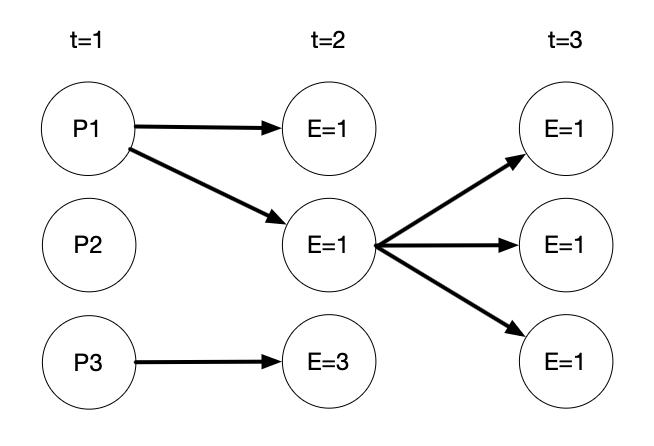
\includegraphics[width=9cm]{eevaindeksit}
\caption{Esimerkki Eeva-indekseistä, kun $T=3$ ja $N=3$.}
\label{fig:eeva-indeksit}
\end{figure}

Varianssiestimaatti voidaan laskea näiden, Leen ja Whitleyn Eeva-indekseiksi nimeämien indeksien perusteella seuraavasti:

\begin{align}\label{CLT-varianssi}
\hat{\sigma}^2_{CLT} = \frac{1}{N^2} \left[ (\sum_{i=1}^N \gamma(x_k^i))^2 - (\frac{N}{N-1})^{n+1} ( \sum_{i=1}^N \sum_{j:E_n^j=i} \gamma(x_k^i) \gamma(x_k^j)) \right]
,\end{align}

missä \(\gamma: \mathbf{X}_n \rightarrow \mathbb{R}\) on rajoitettu, \(\mathcal{X}_n\)-mitallinen funktio. SIR-algoritmin kohdalla jakaumaestimaatti \(\hat{p}(x_{1:k}|y_{1:k}))\). Kyseessä on harhaton ja konsistentti asymptoottisen varianssin estimaatti. Tarkemmin \(N\hat{\sigma}^2_{CLT}\) konvergoi asymptoottiseen varianssiin \ref{asymptoottinen-varianssi}. Tätä ei tutkielman puitteissa todisteta.

Yllä esitetty varianssiestimaatti kärsii kuitenkin epätarkkuudesta, sillä kun \(k \to \infty\) polveutuvat kaikki hiukkaset lopulta samasta kantaisästä eli indeksit \(E_k^i,\ldots,E_k^N\) ovat kaikki yhtäsuuria. Tämän vuoksi on mielekästä johtaa indeksit ainoastaan tietystä aiemmasta ajanhetkestä alkaen. Olsson ja Douc (2019) \citep{olsson-2019} ehdottavat tähän tarkoitukseen Henok-indeksiä \(E_{k,m}^n\), jossa \(m\) merkitsee ajanhetken \(m<k\) partikkelia, josta kyseinen partikkeli polveutuu. Partikkelien kantaisien sukupolvi määritetään viipeellä \(\lambda\) niin, että \(m=k-\lambda\). Kaavio \ref{fig:henok-indeksit} havainnollistaa partikkelien polveutumista, kun \(\lambda=1\).

\begin{figure}[H]
\centering
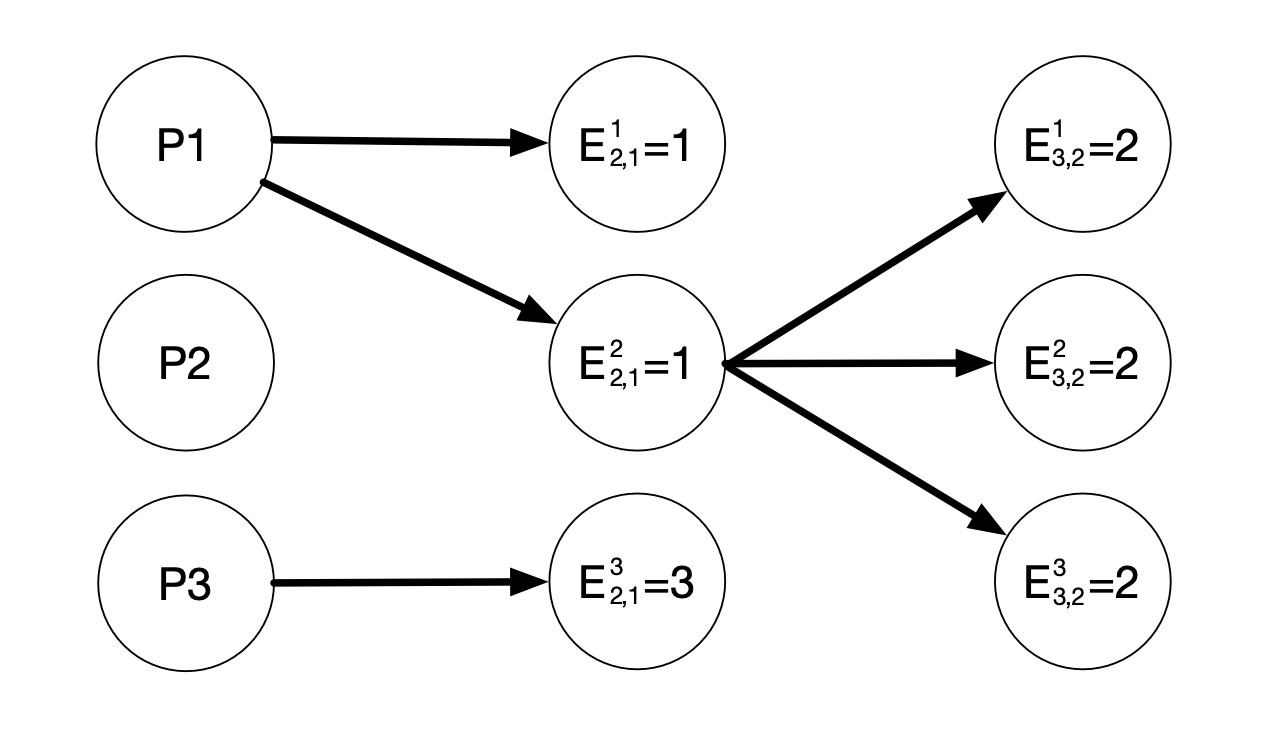
\includegraphics[width=9cm]{henokindeksit}
\caption{Esimerkki Henok-indekseistä, kun $T=3$, $N=3$ ja $\lambda=1$.}
\label{fig:henok-indeksit}
\end{figure}

Nyt varianssi saadaan muotoon

\begin{align}\label{OD-varianssi}
\hat{\sigma}^2_{OD} = \frac{1}{N^2} \left[ (\sum_{i=1}^N \gamma(x_k^i))^2 - (\frac{N}{N-1})^{n+1} ( \sum_{i=1}^N \sum_{j:E_{n,k(\lambda)}^j=i} \gamma(x_k^i) \gamma(x_k^j)) \right]
,\end{align}

missä \(k(\lambda) \vcentcolon= k-\lambda\). Viive \(\lambda\) on varianssiestimaatin suunnitteluparametri. Pienillä viipeillä estimaatti on harhainen, mutta harha laskee viipeen kasvaessa. Olsson ja Douc suosittavat viipeen ylärajaksi arvoa \(\lambda=20\), jolloin estimaattorin harha on käytännössä kokonaan hävitetty. Tämän jälkeen estimaatti voi myös alkaa kärsiä samasta epätarkkuudesta kuin Eeva-indekseihin perustuva CLT-estimaatti.

Mastrototaro ja Olsson (2023) \citep{Mastrototaro-2023} laajentavat tätä estimaattia edelleen niin, että viive \(\lambda\) valitaan mukautuvasti. Mastrototaron ja Olssonin ALvar-estimaatti (\emph{Adaptive-Lag variance}) lasketaan, kuten OD-varianssi edellä \ref{OD-varianssi}, mutta kunkin algoritmin ajokerran jälkeen asetetaan seuraavan ajanhetken \(\lambda\) seuraavasti:

\begin{align}\label{ALvar-lambda}
\lambda_{k+1} \leftarrow \operatorname*{arg\,max}_{\lambda \in [0, \lambda_k + 1]} \hat{\sigma}^2_{k+1,\lambda} (\gamma_{k+1})
,\end{align}

Tämä perustuu havaintoon, jonka mukaan ehtyneille Henok-indekseille on olemassa \(\lambda^\prime \in [0, \lambda-1]\), joka täyttää ehdon \(\hat{\sigma}^2_{k+1,\lambda} (\gamma_{k+1}) < \hat{\sigma}^2_{k+1,\lambda^\prime} (\gamma_{k+1})\), koska myös ehtyneiden indeksien kantaisät ovat ehtyneitä. Nyt indeksi \(\lambda_{n+1}\) voidaan valita rekursiivisesti niin, että se tuottaa suurimman varianssiestimaatin, joka on kuitenkin rajoitettu ylhäältä arvoon \(\lambda_n+1\). Tämä indeksi ei ole koskaan ehtynyt, joten se on myös parhaan varianssiestimaatin tuottava valinta.

Esitettyjä varianssiestimaatteja voidaan hyödyntää paitsi algoritmien ja parametrivalintojen vertailussa myös mukautuvan viipeen hiukkassiloittimen viipeen valinnassa (kts. luku \ref{hiukkassiloittimet}). Varianssiestimaattia hyödynnetään myös luvun \ref{paikannusesimerkki} empiirisen esimerkin uskottavuusfunktioiden parametrien estimoinnissa.

\chapter{Hiukkassilottimet} \label{hiukkassiloittimet}

Tässä luvussa käsitellään suodinongelmaan läheisesti liittyvän hiukkassiloittimen ratkaisemista ns. hiukkassiloitinalgoritmien avulla. Kuten hiukkassuotimien kohdalla, myös tässä luvussa esitetään ongelma ensin yleisessä Bayesilaisessa muodossa, jonka jälkeen siirrytään käsittelemään hiukkasmenetelmiin pohjautuvia siloitinalgoritmeja. Luvussa käsiteltävät algoritmit jaetaan kahteen pääkategoriaan, offline-algoritmeihin, joita sovelletaan hiukkassuodinalgoritmin ajon jälkeen sekä online-algoritmeihin, jotka suoritetaan yhdessä hiukkassuodinalgoritmin kanssa.

Siloitinongelman esittely seuraa Särkkää (2013) \citep{sarkka-2013}. Algoritmien käsittely pohjautuu SIR- ja BS-PS-siloittimien osalta Särkkään (2013) \citep{sarkka-2013} sekä SIR-siloittimen osalta Genshiro Kitagawan artikkeliin ``Monte carlo filter and smoother for non-gaussian nonlinear state space models'' (1996) \citep{kitagawa-1996}. Kiinteän viipeen silotin seuraa niin ikään Kitagawaa (1996). Uudelleenpainottava siloitin perustuu Doucet \&al.~artikkeliin ``On sequential Monte Carlo sampling methods for Bayesian filtering'' (2000) \citep{Doucet-2000}. Mukautuvan viipeen siloitin seuraa puolestaan Alenlövin ja Olssonin artikkelia ``Particle-Based Adaptive-Lag Online Marginal Smoothing in General State-Space Models'' (2019) \citep{alenlov-2019}.

\section{Bayesilainen siloitin}

Bayesilaisen siloittimen tarkoitus on laskea tilan \(x_k\) marginaaliposteriorijakauma \(p(x_k|y_{1:T}\) ajanhetkellä \(k\), kun käytössä on havaintoja ajanhetkeen \(T\) asti, missä \(T>k\). Ero Bayesilaiseen suotimeen (kts. alaluku \ref{bayesilainen-suodin}) on siinä, että suodinongelmassa havaintoja on saatavilla ainoastaan ajanhetkeen \(k\) asti, kun taas siloitinongelmassa myös tulevat havainnot ovat saatavilla. Ajassa taaksepäin etenevät rekursiiviset yhtälöt ongelman ratkaisemiseksi voidaan esittää muodossa

\begin{align}\label{siloitin-prediktiivinen}
p(x_{k+1}|y_{1:k})=\int_{\mathbb{R}^{n_x}}p(x_{k+1}|x_k)p(x_k|y_{1:k})\mathop{dx_k}.
\end{align}

\begin{align}\label{siloitin-ratkaisu}
p(x_k|y_{1:T}) = p(x_k|y_{1:k}) \int \frac{p(x_{k+1}|x_k)p(x_{k+1}|y_{1:T})}{p(x_{k+1}|y_{1:k})} \mathop{dx_{k+1}}.
\end{align},

missä \(p(x_k|y_{1:k})\) on suodintiheys ajanhetkellä \(k\) ja \(p(x_{k+1}|y_{1:k})\) prediktiivinen jakauma ajanhetkelle \(k+1\). Kuten suodinongelman kohdalla, voidaan ongelma ratkaista suljetussa muodossa, kun mallit ovat lineaarisia. Tällöin kyseessä on Rauch-Turn-Striebel-siloitin (RTSS), josta käytetään myös nimitystä Kalman-siloitin. Samoin, kuten Kalman-suotimen kohdalla, ongelma voidaan tiettyjen ehtojen vallitessa linearisoida. Näitä linearisoituja suodattimia ei käsitellä tässä tutkielmassa. hiukkassuotimen tavoin hiukkassiloitin ratkaisee ongelman mille hyvänsä epälineaariselle mallille.

\section{Offline-algoritmit}

Offline-siloittimet estimoivat siloitintiheyttä ajanhetkellä \(k<T\), kun havaintodata on käytössä koko ajanjaksolta \(1 \ldots T\). Alla esitetyt algoritmit siis olettavat, että kaikki mahdollinen tuleva data on jo niiden käytössä. Ohessa käsitellään lyhyesti muutamaa ehdotettua offline-hiukkassiloitinalgoritmia.

\subsection{SIR-siloitin}

Kuten aiemmin mainittua, näyttävät hiukkassuodinalgoritmit, erityisesti SIR-algoritmi \ref{sir}, ratkaisevan siloitteluongelman ilmaiseksi, kunhan tallennamme ajanhetkellä \(k\) koko otoshistorian \(x_{0:k}^i\). Tällöin voimme estimoida täyttä siloitteluposteriorijakaumaa seuraavasti:

\begin{align}\label{siloitin-posteriori}
p(x_{0:T}|y_{1:T}) \approx \sum_{i=1}^N w_T^i \delta (x_{0:T}-x_{0:T}^i).
\end{align}

Nyt ajanhetken \(k\) siloitinjakauma saadaan laskettua

\begin{align}\label{siloitin-posteriori-k}
p(x_{k}|y_{1:T}) \approx \sum_{i=1}^N w_T^i \delta (x_{k}-x_{k}^i),
\end{align}

missä \(x^i_k\) on \(x^i_{0:T}\):n \(k\):s elementti. Koska uudelleenotanta hävittää otoshistorian, pitää uudelleenotanta suorittaa koko otoshistoriasta \(x_{0:k}^i = (x_{0:k-1}^i, x_{k}^i)\) pelkän ajanhetken \(k\) otoksen \(x_{k}^i\) sijaan. Koska nyt koko otoshistoria pitää tallentaa, vaatii SIR-siloitin \(NkT\) muistia pelkän \(N\) sijaan. Vastaavasti myös uudelleenotannan aikakompleksisuus kasvaa. \citep{kitagawa-1996}

SIR-siloittimen suurin ongelma on kuitenkin sen tuottamien estimaattien hyvyys. Kun ajanhetkien määrä kasvaa, johtaa koko otoshistorian uudelleenotanta kaiken painon kasautumiseen historian tietyille otoksille, jolloin SIR-siloittimen tuottamat estimaatit eivät enää estimoi haluttua (siloittelu)posteriorijakaumaa. \citep{kitagawa-1996}

\subsection{BS-PS-siloitin}

\emph{Backward-simulation particle smoother} (BS-PS) eli taaksepäin simuloiva hiukkassiloitin estimoi paremmin hiukkassuotimen tulosten perusteella siloitinjakaumaa. Tässä algoritmissa hiukkasten historia simuloidaan ajanhetkestä \(T\) taaksepäin ajanhetkeen 0:

\begin{algorithm}[H]
\label{BSPS}
\DontPrintSemicolon
\SetAlgoShortEnd
\KwResult{Posteriorisiloitinjakauman $p(x_{k}|y_{1:T})$ estimaatti.\;}
\KwData{Suodinjakaumia edustavat hiukkaset ja näihin liittyvät painot ${w_k^i, x_k^i}$, missä $i=1,\ldots,N$ ja $k=1,\ldots,T$\;}
\Begin{
  \Begin{Valitaan $\tilde{x}_T=x_T^i$\;}
  \For{$k=\{T-1,\ldots,0\}$}{
    \Begin{Lasketaan uudet painot \newline $w^i_{k|k+1} \propto w_k^i p(\tilde{x}_{k+1}|x_k^i)$\;}
    \Begin{Valitaan $\tilde{x}_{k} = x_k^i$ todennäköisyydellä $w^i_{k|k+1}$.\;}
  }  
}
\caption{Taaksepäin simuloiva hiukkassiloitin}
\end{algorithm}

Nyt siloittelujakaumaa voidaan estimoida seuraavasti:

\begin{align}\label{siloitin-BSPS}
p(x_{0:T}|y_{1:T}) \approx \frac{1}{S} \sum_{i=1}^N \delta (x_{0:T}-\tilde{x}_{0:T}^j),
\end{align}

missä \(S, j=1,\ldots,S\) on algoritmin \ref{BSPS} toistokertojen määrä. Koska \(\tilde{x}_{0:T}^j\) pitää sisällään kaikki otospolut, saadaan marginaalijakauma ajanhetkellä \(k\) yhtälöstä \ref{siloitin-BSPS} yksinkertaisesti valitsemalla sen \(k\):net elementit. Sekä algoritmin aikakompleksisuus että muistivaade on \(\mathcal{O}(STN)\).

\subsection{Uudelleenpainottava hiukkassiloitin}

Uudelleenpainottavassa hiukkassiloittimessa (tunnetaan myös nimellä marginaalihiukkassiloitin, kts. mm. Doucet, Godsill \& ja Andrieu \citep{Doucet-2000}) siloitinjakaumaa estimoidaan käyttämällä SIR-hiukkassuodattmista (\ref{sir}) saatuja hiukkasia, mutta ne painotetaan uudelleen käyttäen dataa ajanhetkestä \(T\) alkaen, edeten ajassa taaksepäin.

\begin{algorithm}[H]
\label{rwps}
\DontPrintSemicolon
\SetAlgoShortEnd
\KwResult{Posteriorisiloitinjakauman $p(x_{k}|y_{1:T})$ estimaatti.\;}
\KwData{Suodinjakaumia edustavat hiukkaset ja näihin liittyvät painot ${w_k^i, x_k^i}$, missä $i=1,\ldots,N$ ja $k=1,\ldots,T$\;}
\Begin{
  \Begin{Asetetaan $w_{T|T}^i = w_T^i$, jokaiselle $i=1,\ldots,N$;}
  \For{$k=\{T-1,\ldots,0\}$}{
    \Begin{Lasketaan uudet painot \newline $w^i_{k|T} = \sum_j w_{k+1|T}^j  \frac{w_k^i p(x_{k+1}^j|x_k^i)}{\sum_l w_k^l p(x_{k+1}^j|x_k^l)}$\;}
  }  
}
\caption{Uudelleenpainottava hiukkassiloitin}
\end{algorithm}

,

jolloin halutun siloitinjakauma estimaatti ajanhetkellä \(k\) saadaan painotettuna keskiarvona \(p(x_k|y_{1:T}) \approx \sum_i w_{k|t}^i \delta (x_k-x_k^i)\). Algoritmin aikakompleksisuus on \(\mathcal{O}(N^2)\).

\section{Online-algoritmit}

Yllä esitetyt offline-suodinongelmat ratkaisevat suodinongelman niin, että kaikki data ajanhetkeen asti \(T\) on saatavilla. Käytännössä siloitin siis ajetaan suodinalgoritmin jälkeen. Käytännön sovelluksissa tämä ei ole aina mahdollista, jos siloittelujakauman pitää olla saatavilla reaaliaikaisesti. Online-siloittimet ratkaisevat nyt siloitinongelman niin, että saatavilla on dataa ajanhetkeen \(k+L \le T\) asti, missä \(L\) on dataan lisätty \(L\):n ajanhetken viive. Online-algoritmit voidaan edelleen jakaa kiinteän viipeen siloittimiin (\emph{fixed-lag smoother}) ja mukautuvan viipeen siloittimiin (\emph{adaptive-lag smoother}). Nimensä mukaisesta kiinteän viipeen siloitinalgoritmeissa viive \(L\) valitaan suunnitteluparametrina, kun taas mukautuvan viipeen siloittimet pyrkivät valitsemaan parhaan tai optimaalisen viipeen johonkin kriteeriin perustuen.

\subsection{Kiinteän viipeen siloitin}

Yksinkertaisin tapa toteuttaa kiinteän viipeen siloitin on yksinkertaisesti käyttää SIR-siloitinta niin, että maksimiajanhetki \(T\) korvataan valitulla viipeellä \(k+L \le T\). \citep{kitagawa-1996}. Nyt yhtälön \ref{siloitin-posteriori} jakauma saadaan muotoon

\begin{align}\label{siloitin-posteriori-viive}
p(x_{0:(k+L)}|y_{1:(k+L)}) \approx \sum_{i=1}^N w_{k+L}^i \delta (x_{0:(k+L)}-x_{0:(k+L)}^i),
\end{align}

ja nykyisen ajanhatken \(k\) siloitinjakauma lasketaan tästä jakaumasta kuten SIR-siloittimessa (kts. yhtälö \ref{siloitin-posteriori-k}). Kiinteän viipeen siloitin myös välttää SIR-siloittimen approksimaatio-ongelmat. Kun viipeelle \(L\) pätee \(k+L \ll T\) parantaa viipeen pidentäminen tiettyyn pisteeseen asti jakauman approksimaatiota. Kitagawa (1996) suosittelee 10\textendash 20 aika-askeleen viivettä ja esittää 50 aika-askelta viipeen ylärajaksi. \citep{kitagawa-1996}. Paremman estimaatin vastapainona pidemmän viipeen valinta lisää myös viivettä, joka dataa tuottavaan järjestelmään pitää lisätä. Siloittimien tulokset ovat saatavilla vasta \(L\) ajanhetken jälkeen, mikä ei aina ole käytännössä mahdollista tai haluttua. Pidempi viive myös lisää algoritmin muistivaatimuksia, joskin muistivaatimukset pysyvät aina pienempinä kuin SIR-siloittimessa.

Kiinteän viipeen siloitinta (viipeellä \(L=1\)) voidaan hyödyntää myös prediktiivisenä siloittimena, jossa siloittelujakaumaa \(p(x_{0:(k+1)}|y_{1:(k+1)}\) käytetään suodinjakauman \(p(x_{1:(k)}|y_{1:k})\) laskennassa. \citep{Nyobe-2021} Ydinajatuksena on muokata SIR-algoritmia \ref{sir} niin, että ajanhetken \(k\) painoja \(w_k^i\) painotetaan edelleen seuraavan ajanhetkestä \(k+1\) lasketuilla painoilla ja näin painottaa jo nykyhetkessä niitä hiukkasia, joiden uskottavuus on seuraavalla ajanhetkellä suurempi. Tämä prediktiivinen siloitin voidaan toteuttaa lisäämällä SIR-algoritmiin painotusvaiheen jälkeen seuraava ala-algoritmi:

\begin{algorithm}[H]
\label{prediktiivinen-siloitin}
\DontPrintSemicolon
\SetAlgoShortEnd
\KwResult{Prediktiivisellä siloittimella lasketut painot painotettu $\tilde{w}_{k}^i$.\;}
\KwData{Viipeen $L=1$ avulla saadut havainnot $y_{k+1}$. Partikkelit $x_k^i$ ja niitä vastaavat painot $w_k^i$\;}
\Begin{
  \For{$i=\{1,2,\ldots,N\}$}{
      \Begin{Luodaan simuloidut hiukkaset $\tilde{x}_{k+1}^i$ ehdotusjakaumsta $q(\tilde{x}_{k+1}|x^i_k,y_{k+1})$\;}
      \Begin{Lasketaan simuloiduille hiukkasille painot $\tilde{w}_{k+1}^i$\;}
      \Begin{Päivitetään nykyiset painot $\tilde{w}_{k}^i = {w}_{k}^i \tilde{w}_{k+1}^i$\;}
    }
  \Begin{Korvataan nykyiset painot ${w}_{k}$ siloitetuilla painoilla $\tilde{w}_{k}^i$;}
  }  
\caption{Prediktiivinen siloitin (viive=1)}
\end{algorithm}

Kun hiukkasten määrä \(N\) pysyy samana, lisää prediktiivinen siloitin suodinjakauman laskemisen tarkkuutta. Vastaavasti prediktiivinen siloitin mahdollistaa saman suodinjakauman estimaatin tarkkuuden kuin SIR-algoritmi pienemmällä määrällä hiukkasia, kuitenkin vain tuplaten uskottavuusfunktiota laskettaessa vaadittavan laskentatehon ja muistitarpeen.

\subsection{Mukautuvan viipeen siloitin}

Yllä esitetyssä kiinteän viipeen siloittimessa on valittu viive \(L\) suunnitteluparametri. Valittu viive on aina kompromissi: liian suuri viive kasvattaa siloitinjakauman estimoinnin epätarkkuutta ja hidastaa laskentaa, kun taas liian pieni viive saattaa johtaa niin ikään epätarkkuuteen. Lisäksi valittu viive ei välttämättä johda jokaisella aika-askeleella optimaaliseen tai edes hyvään laskentatulokseen. Mukautuvan viipeen siloittimet yrittävät ratkaista tämän ongelman mukauttamalla kunakin ajanhetkenä valittua viivettä johonkin kriteeriin perustuen. Erään version mukautuvan viipeen siloittimesta esittävät Johan Alenlöv ja Jimmy Olsson artikkelissa ``Particle-Based Adaptive-Lag Online Marginal Smoothing in General State-Space Models'' (2019) \citep{alenlov-2019}. Siloitin hyödyntää hiukkassuotimen varianssiestimaattia viipeen valinnassa.

Yksinkertaisin versio siloittimesta on esitetty algoritmissa \ref{mukautuva-siloitin}. Perusidea on viivästyttää siloitinjakauman luomista hetkellä \(k\), kunnes tarjolla on viipeet \(S=1,\ldots,s\), joiden varianssi

\begin{align}\label{siloitin-varianssi}
\sigma^2_{s|t} = \sum_{i=1}^N \frac{w_t^i}{\Omega_t}\left\{\tilde{x}_{s|t} - \sum_{j=1}^N \frac{w_t^j}{\Omega_t}\tilde{x}_{s|t} \right\}^2,
\end{align}

pysyy tietyn valitun rajan \(\epsilon\) yläpuolella, missä \(\tilde{x}_{s|t}\) on kyseiselle viipeellä laskettu marginaalisiloitinjakauman painovektori (kts. algoritmi \ref{rwps}). Kun tämä ehto ei enää täyty, käytetään suurimmalle kriteerin \(\sigma^2{s|t} < \epsilon\) täyttämälle viipeelle laskettuja painoja siloitinjakauman estimointiin kaikilla \(t^\prime \ge t\). Varianssin estimoinnista katso alaluku \ref{varianssin-estimointi}.

\begin{algorithm}[H]
\label{mukautuva-siloitin}
\DontPrintSemicolon
\SetAlgoShortEnd
\KwResult{Siloittelujakauman estimaatti viipeellä $s$, tarkemmin $\sum_i^N w_t^i \tilde{x}_{s|t}^i \Omega_t$.\;}
\KwData{Olkoon $S$ joukko kullakin viipeellä $s$ laskettuja painoja $\tilde{x}_{s|t}^i$. Alustetaan $S \leftarrow \emptyset$\;}
\Begin{
  \For{$t=\{1,2,\ldots,T\}$}{
      \Begin{Ajetaan SIR-algoritmi \ref{sir} ajanhetkenä $t$\;}
      \Begin{Jokaiselle $s \in S$ lasketaan painovektori kuten algoritmissa \ref{rwps}.\;}
      \Begin{$S \leftarrow S \cup \{s\}$Jokaiselle $s \in S$ lasketaan painovektori kuten algoritmissa \ref{rwps}.\;}
      \Begin{Jokaiselle $s$ lasketaan varianssi $\sigma^2_{s|t}$ kuten yhtälössä \ref{siloitin-varianssi}. Jos $\sigma^2_{s|t} < \epsilon$ poistetaan $s$ joukosta $S$ ja käytetään siloitinjaukauman estimaattia $\sum_i^N w_t^i \tilde{x}_{s|t}^i \Omega_t$ kaikille ajanhetkille $t^\prime \ge t$.\;}
    }
  }  
\caption{Mukautuvan viipeen siloitin}
\end{algorithm}

Myös tähän siloittimeen liittyy suunnitteluparametrien valinta. Vaikka itse viivettä \(L\) ei valita, pitää parametri \(\epsilon\). Pienempi \(\epsilon\) tuottaa suurempia viipeitä ja täten parempia estimaatteja, mutta on myös laskennallisesti sekä muistin käytöltään raskaampi. Alenlöv ja Olsson ehdottavat \(\epsilon\)-arvoja väliltä \((.5, 10^{-3})\).

\chapter{Hiukassuodin ja -siloitin sisätilapaikannuksessa} \label{paikannusesimerkki}

Sisätilapaikannus tarkoittaa nimensä mukaisesti ihmisten tai esineiden automaattista paikantamista sisätiloissa. Koska GPS-järjestelmät toimivat sisätiloissa huonosti tai eivät lainkaan, tarvitaan rakennusympäristöihin muita paikannusratkaisuja. Tässä luvussa käydään ensin läpi sisätilapaikannuksen yleisiä periaatteita sekä joitakin ehdotettuja ratkaisuja. Lisäksi mainitaan joitakin hiukassuodinalgoritmin käyttötapoja sisätilapaikannuksessa. Tämän jälkeen keskitytään Walkbase-ohjelmistoyrityksen sisätilapaikannusteknologian ympärille kehitettyyn algoritmiin, jonka tarkkuutta ja tehokkuutta testataan koeympäristössä.

\section{Sisätilapaikannuksesta}

Sisätilapaikannus tarkoittaa tekniikoita ja menetelmiä, joilla paikannetaan ihmisiä, laitteita tai esineitä sisätiloissa, joissa perinteinen GPS-signaali ei ole riittävä tai saatavilla. Sisätilapaikannuksessa hyödynnetään useita erilaisia teknologioita, kuten radiotaajuuksia, magneettikenttiä, ultraääntä ja optisia menetelmiä. Kattava esitys sisätilapaikannukseen käytettävistä teknologioista löytyy George Ogunatalan \&al.~artikkelista ``Indoor location identification technologies for real-time IoT-based applications: An inclusive survey'' (2018) \citep{oguntala-2018}, johon myös tämä alaluku perustuu.

Optisessa paikannuksessa käytetään kameroita tai muita optisia/valoon perustuvia sensoreita, kuten esimerkiksi Lidar-valotutkia, halutun kohteen sijainnin määrittämiseen. Magneettikenttiin perustuvat paikannusratkaisut perustuvat rakennusten sisäisten metallirakenteiden maapallon magneettikenttään luomiin paikallisiin muutoksiin. Näitä muutoksia voidaan käyttää vertailutietona paikannuksessa, mittaamalla ympäröivän magneettikentän vahvuutta ja vertaamalla sitä ennalta tallennettuihin karttoihin. Ultraäänipohjainen paikannus puolestaan hyödyntää ääniaaltojen kulkuaikaa lähettimen ja vastaanottimen välillä.

Yleinen valinta sisätilapaikannuksessa ovat erilaiset Bluetooth-standardiin tai muuhun radioteknologiaan (kuten esimerkiksi millimetriaaltoihin) perustuvat lähetin-vastaanotinratkaisut, joissa hyödynnetään laitteiden välisiä signaaleja etäisyyden tai kulman mittaamiseen. Radioteknologiaan perustuvilla järjestelmillä voidaan kotuullisin kustannuksin saavuttaa jopa senttimetritason paikannustarkkuus tietyissä sovelluksissa. Radioteknologiat ovat myös yksityisyyden näkökulmasta helpompia järjestelmiä toteuttaa kuin esimerkiksi kameroiden avulla tapahtuvaan paikannukseen perustuvat järjestelmät.

\section{Teknologian kuvaus}

Turkulainen teknologia- ja analytiikkayritys Walkbase käyttää Bluetooth/BLE-sisätilapaikannusta asiakkaiden käyttäytymistä koskevan datan keräämiseen erityisesti ruokakaupoissa sekä tavarataloissa. Tyypillisessä asennusskenaariossa lähettimet (tagit) kiinnitetään ostoskärryihin ja paikantimet kiinnitetään liiketilan kattoripustuksiin.

Walkbase on kehittänyt sisätilapaikannukseen oman laitteisto- ja ohjelmistoratkaisunsa, jonka tavoitteena on tarjota kaikissa ympäristöissä \(95\%\) varmuudella alle metrin paikannustarkkuus. Koska tagit kiinnitetään tunnetulle korkeudelle ostoskärryihin, riittää paikannusvirhettä laskiessa tarkastella ainoastaan leveys- ja pituusasteita. Kun tagin todellinen sijainti \(P_k=(P_{\text{lon}_k}, P_{\text{lat}_k})\) tiedetään aika-askeleella \(k\), voidaan sijaintiestimaatin \(\hat{x}_k=(\hat{x}_{\text{lon}_k}, \hat{x}_{\text{lat}_k})\) Merkitään tätä paikannusvirhettä yksittäisen sijainnin kohdalla

\begin{align}\label{paikannusvirhe}
\epsilon_{\text{pos}_k} = d(P_k,\hat{x}_k) = \sqrt{(P_{\text{lon}_k}-\hat{x}_{\text{lon}_k})^2+(P_{\text{lat}_k}-\hat{x}_{\text{lat}_k})^2}
,\end{align}

eli käytetään paikannusvirheenä yksinkertaisesti euklidista etäisyyttä. Tämä antaa paikannusvirheen suoraan metreinä alaluvussa \ref{karttaprojektioista} suoritettavan lineaarisen interpolaation vuoksi. Haluttu, alle metrin paikannustarkkuus saavutetaan, kun missä hyvänsä testiasetelmassa kaikkien asetelmaan liittyvien paikannusvirheiden \(50.\) persentiili on \(\leq1\)m.

Walkbasen paikannusratkaisu koostuu kolmesta eri laitteistokomponentista, AT-2-Bluetooth-lähetin-vastaanottomista, jotka kiinnitetään ostoskärryihin, XR-2-Bluetooth-lähetin-vastaanottomista, jotka kiinnitetään tilan kattoripustuksiin sekä OSCU-laskentayksiköstä, joka luo paikkadataa XR-2.1-vastaanotinten perusteella ja lähettää paikkadatan edelleen palvelinkeskukseen.

AT-2 on Bluetooth 5.1 (BLE) -strandardin mukaan toimiva lähetin-vastaanotin, joka toimii 2.4Ghz taajuusalueella. Walkbasen suunnitteleman laitteen PCB-kehäantenni kykenee lähettämään GFSK-moduloitua dataa 2Mbps nopeudella. Laite saa virtansa yhdestä CR-2477-paristosta.

XR-2.1 on Bluetooth 5.1 (BLE) -strandardin mukaan toimiva lähetin-vastaanotin, joka toimii 2.4Ghz taajuusalueella. Walkbasen suunnitteleman laitteenPCB-kehäantenni kykenee lähettämään GFSK-moduloitua dataa 2Mbps nopeudella. Laite saa virtansa ethernet-lähiverkosta 802.3af-standardin mukaisesti. Laitteen vaatima laskenta tapahtuu Raspberry Pi Compute Module 4 -piirilevytietokoneella. Lisäksi laite sisältää inertiamittausyksikön, jota voidaan käyttää asennetun laitteen kallistumis- ja nyökkäämiskulman (\emph{roll} ja \emph{pitch}) arviomiseen.

OSCU-laskentayksikkönä käytetään Ubuntu-käyttöjärjestelmällä toimivaa tietokonetta. Koska OSCU-laskentayksikön laskentateho on rajallista, on paikannusalgoritmin aikakompleksisuus yksi käytettävän algoritmin ydinkriteereistä.

Tarvittavasta laskennasta vastaava ohjelmistojärjestelmä koostuu puolestaan neljästä ohjelmistokomponentista. C-ohjelmointikielellä toteutettu \emph{angler} laskee AT-2-tagin lähettämän I/Q-datan perusteella signaalien tulokulman, Go-ohjelmointikielellä toteutettu \emph{moonraker} lähettää tulokulmadatan paikallisverkon yli OSCU-laskentayksikölle, jossa Go-ohjelmointikielellä toteutettu \emph{launchpad} luo siitä sijaintidataa, jonka se lähettää edelleen palvelinkeskuksen taustajärjestelmään.

Taustajärjestelmässä Go-ohjelmointikielellä \emph{goldfinger} prosessoi sijaintidatan Walkbasen analytiikka-alustan käyttämään muotoon. \emph{Goldfinger} myös vastaa siitä, että kaikki \emph{launchpad}-sovelluksen vaatima metadata on sen käytössä. Kaavio \ref{fig:jarjestelmaarkkitehtuuri} kuvaa järjestelmän laitteisto- ja ohjelmistoarkkitehtuurit.

\begin{figure}[H]
\centering
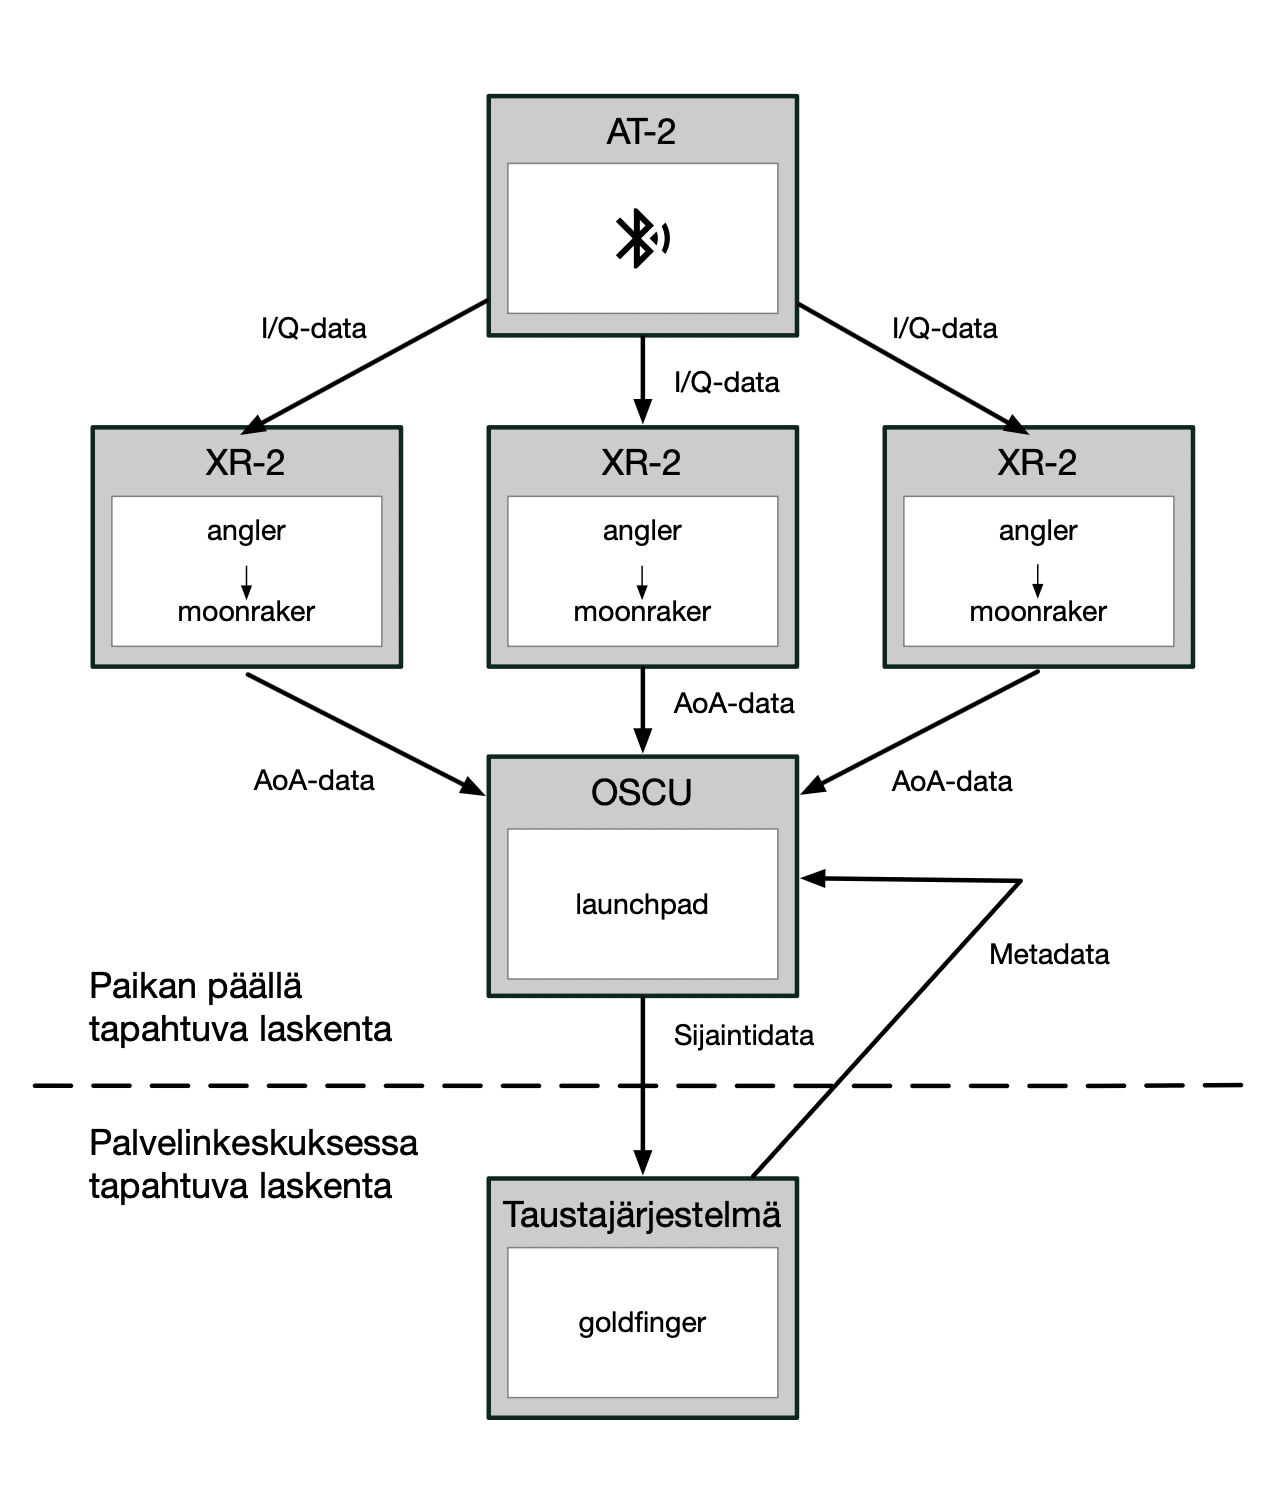
\includegraphics[width=15cm]{jarjestelmaarkkitehtuuri}
\caption{Järjestelmäarkkitehtuuri}
\label{fig:jarjestelmaarkkitehtuuri}
\end{figure}

Tässä luvussa keskitytään \emph{launchpad}-sovelluksen hyödyntämään paikannusalgoritmiin, mutta sitä ennen käsitellään lyhyesti tulokulman laskentamenetelmät sekä \emph{angler}-sovelluksen toiminta. Tekijänoikeussyistä tutkielmassa ei hyödynnetä Go-ohjelmointikielellä toteutettua ohjelmakoodia. Sen sijaan algoritmi on toteutettu R-ohjelmointikielellä.

\subsection{AoA-menetelmistä} \label{aoa}

Riippuen käytetystä teknologiasta ja teknologian tuottamasta datasta, voidaan sisätilapaikannuksessa soveltaa lukuisia eri paikannustekniikkoja ja -algoritmeja. Oguntalaa (2018) \citep{oguntala-2018} mukailevassa kaaviossa \ref{fig:paikannusmenetelmat} on esitetty pääpiirteittäin sisätilapaikannusmenetelmät käytetyn datan (kaaviossa oikealla) mukaan jaoteltuna.

\begin{figure}[H]
\centering
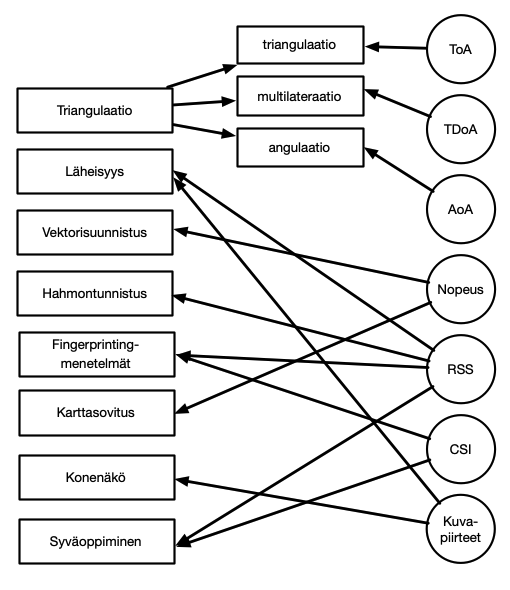
\includegraphics[width=12.5cm]{paikannusmenetelmat}
\caption{Paikannusmenetelmien luokittelu}
\label{fig:paikannusmenetelmat}
\end{figure}

Walkbasen toteuttama paikannusratkaisu perustuu AoA-menetelmään. Tämä on paikannusteknologia, joissa lähettimen ja vastaanottimen välinen kulma estimoidaan signaalin saapumiskulman perusteella. Tässä estimoinnissa hyödynnetään signaalin vaihe-eroja, kun sama signaali vastaanotetaan usealla eri antennilla.

Walkbase hyödyntää radiosignaalien tulokulman estimoinnissa MUSIC-algoritmia (\emph{Multiple Signal Classification}), joka arvioi tulokulmia analysoimalla signaalien autokorrelaatiomatriisia ja etsimällä sen ominaisvektoreita. Esitys MUSIC-algoritmista löytyy esimerkiksi Monson H. Hayesin kirjasta \emph{Statistical Digital Signal Processing and Modeling} (1996) \citep{Hayes-1996}. Marco Guniam \&al (2023) \citep{Gunia-2023} puolestaan esittävät artikkelissa ``Analysis and Design of a MuSiC-Based Angle of Arrival Positioning System'' tapoja optimoida MUSIC-algoritmia soveltumaan monimutkaisiin, heijastuksia sisältäviin sisätilaympäristöihin.

\emph{angler}-sovellus hyödyntää MUSIC-algoritmin ohella omaa hiukassuodinalgoritmiaan signaalispektrin analysointiin sekä tulokulmien estimointiin. MUSIC-algoritmia tai \emph{angler}-sovelluksen hiukassuodinalgoritmia ei käsitellä tarkemmin tämän tutkielman puitteissa.

\subsection{Kalibraatiosta}

Koska \emph{angler}-sovellus laskee suuntimakulman aina antennielementin määrätystä reunasta nähden, on tärkeää, että laitteen asemointi karttapohjoiseen nähden on tiedossa. Koska laitteen tarkan kulman arvioiminen asennusympäristössä on haastavaa eikä laite sisällä kompassia, sovelletaan kunkin laitteen kalibraatioon omaa SIR-algoritmiaan, jonka on mahdollista huomioon myös laitteen IMU-intertiamittausyksiköstä saatavat kallistumis- ja nyökkäämiskulmat.

Jos IMU-dataa hyödynnetään, tuottaa kalibraatioalgoritmi jokaiselle XR-2-laitteelle rotaatiomatriisin \(R_l\). Muussa tapauksessa kalibraatioalgoritmi tuottaa jokaiselle laitteelle atsimuuttiakulman kohdistuksen \(\eta\). Kalibraatioalgoritmia ei käsitellä tämän tutkielman puitteissa. Paikannusongelman yksinkertaistamiseksi myöskään IMU-yksikön tuottamaa dataa ei sisällytetä kalibraatioon ja jokaisen XR-2-laitteen oletetaan olevan lattiaan nähden vaakatasossa. Atsimuuttikulman kalibraatiokohdistuksesta lisää luvussa \ref{datan-kuvaus} alla.

\section{Datan kuvaus} \label{datan-kuvaus}

Koeasetelmaa varten AT-2-tagi on asetettu lähettämään IQ-dataotoksia 6hz taajuudella, joka vastaa järjestelmän tuotantokäyttöä. Parempi sijaintitarkkuus saavutettaisiin korkeammalla taajuudella, mutta käytettyjen tagien akun kesto ei salli 6hz korkeampaa taajuutta.

\emph{angler}-sovellus koostaa jokaisesta aika-askeleen \(k\) dataotoksesta atsimuutti- eli suuntimakulman \(\theta_k\) ja korkeuskulman \(\gamma_k\), jotka noudattavat seuraavia jakaumia:

\begin{align}
&\theta_{k} \sim \text{von Mises}(\mu_{\theta_k}, \kappa_k),\\
&\gamma_{k} \sim \mathcal{N}_{\text{katkaistu}} (\mu_{\gamma_k}, \sigma^2_k).
\end{align}

Nämä on kuvattu tarkemmin alaluvussa \ref{uskottavuusmallit}. Jokaisen XR-2-laitteen \emph{angler}-sovellus laskee näiden perusteella sekvenssinumeron, jonka perusteella samasta AT-2-tagin lähettämästä IQ-dataoksesta lasketut usean eri vastaanottimen laskemat tulokulmat voidaan yhdistää samaan IQ-dataotokseen. XR-2-laitteen lähettämä tulokulmadata on kuvattu alla.

\def\arraystretch{1.25} 
\begin{table}[H]
\centering
\begin{tabular}{|l|l|l|}
\hline
Muuttuja & Kuvaus & Esimerkkiarvo\\
\hline
id & havainnon yksilöivä tunniste & 317,092 \\
ts & havainnon aikaleima & \makecell[l]{2024-04-08 \\ 21:38:20.998+00}\\
locator\_mac & XR-2-laitteen MAC-osoite & 2c:e3:10:00:07:a6
\\
asset\_tag\_mac & AT-2-tagin MAC-osoite & 2c:e3:10:00:63:89\\
sequence\_nr & \makecell[l]{kulmadatan IQ-dataotokseen yhdistävä \\ juokseva numerointi} & 2,066\\
azimuth\_location & \makecell[l]{atsimuuttikulman $\theta$ \\ jaukauman sijaintiparametri $\mu_{\theta}$ (rad)} & 0.39
\\
azimuth\_scale & \makecell[l]{atsimuuttikulman $\theta$ \\ jaukauman skaalaparametri $\kappa$} & 80.98
\\
elevation\_location & \makecell[l]{korkeuskulman $\gamma$ \\ jaukauman sijaintiparametri $\mu_{\gamma}$ (rad)} & 0.13
\\
elevation\_scale & \makecell[l]{korkeuskulman $\gamma$ \\ jaukauman skaalaparametri $\sigma^2$} & 0.012
\\
quality\_sndr & signaali-kohinasuhde & 22.0 \\
rssi & signaalin vahvuus (dBm) & -81\\
distance & arvioitu etäisyys lähettimeen (m) & 18.6\\
\hline
\end{tabular}
\caption{Tulokulmamuuttujat}
\label{tab:aoa-muuttujat}
\end{table}

Etäisyys on estimoitu signaalin vahvuudesta käyttäen propagaatiomallia. Etäisyyttä tai signaalin vahvuutta ei käytetä paikantamiseen, joten tämän mallin käsittely jätetään tutkielman ulkopuolelle. Munoz (2009) luku 2 sisältää yleiskatsauksen propagaatiomalleista. \citep{Munoz-2009}

\emph{launchpad}-sovelluksessa tulokulmadataan yhdistetään XR-2-laitteen MAC-osoitteen perusteella lisäksi tarvittavaa, XR-2-laitteita koskevaa metadataa. Näihin kuuluvat laitteen korkeus, laitteen suuntimakulma ja karttakoordinaatit. Metadata on kuvattu taulukossa \ref{tab:metadata}.

\def\arraystretch{1.25} 
\begin{table}[H]
\centering
\begin{tabular}{|l|l|l|}
\hline
Muuttuja & Kuvaus & Esimerkkiarvo\\
\hline
locator\_mac & XR-2-laitteen MAC-osoite & b8:27:eb:66:0d:2a\\
lat & vastaanottimen sijainti (leveyspiiri) & 60.448265\\
lon & vastaanottimen sijainti (pituuspiirit) & 22.294823\\
direction & suuntimakulma $\eta$ (astetta) & 34\\
height & vastaanottimen korkeus (m) & 2.22 \\
\hline
\end{tabular}
\caption{Metadata}
\label{tab:metadata}
\end{table}

Atsimuuttikulma \(\phi\) lasketaan aina vastaanottimen tietyltä sivulta, joten se vastaa napapohjoista ainoastaan siinä tapauksessa, että vastaanottimen kyseinen sivu on asetettu kohtisuoraan napapohjoiseen nähden. Käytännössä vastaanottimien asettaminen tiettyyn kulmaan ei ole aina mahdollista eikä vaihe-erojen mittaamisen kannalta edes suotavaa. Tämän vuoksi jokaiselle vastaanottimelle on tietokantaan tallennettu oma suuntimakulma \(\eta\). Toisin kuin tulokulmadatan kulmat, on tämä tallennettu tietokantaan asteina. Kokeessa käytetään napapohjoisesta laskettuja kulmia \(\Phi\), jotka lasketaan jokaiselle havainnolle havainnon vastaanottimen suuntimakulman avulla

\begin{align}
\Phi=(\theta + \eta \times \frac{\pi}{180^\degree}) \mod 2 \pi.
\end{align}

Suuntimakulma \(\Phi\) kertoo vastaanottimen ja lähettimen välisen kulman. Lisäksi saatavilla on PostGIS-muotoon tallennettua polygonidataa, joka vastaa koeympäristön pohjapiirrustusta sekä koeympäristössä esiintyviä liikkumisen estäviä kohteita, kuten hyllyjä tai pöytiä. Näitä hyödynnetään sekä sijaintialgoritmin alustuksessa että karttasovitusalgoritmissa (kts. alaluku \ref{karttasovitusalgoritmi})

Havaintomuuttujien ohella koetilanteesta on tallennettu testipolku, jota pitkin AT-2-tagia liikutetaan koetilanteessa. Testipolkudata pitää sisällään karttaan piirretyn janan pääte- ja sisäpisteet. Tallennettu sijainti perustuu koeympäristön lattiaan pohjapiirrustusten sekä laser-mittausten avulla tehtyihin merkintöihin. Näin saadut testimuuttujat on kuvattu taulukossa (\ref{tab:testimuuttujat}).

\def\arraystretch{1.25} 
\begin{table}[H]
\centering
\begin{tabular}{|l|l|l|}
\hline
Muuttuja & Kuvaus & Esimerkkiarvo\\
\hline
path\_lat & polkupisteen sijainti (leveyspiiri) & 60.44819 \\
path\_lon & polkupisteen sijainti (pituuspiiri) & 22.29493 \\
\hline
\end{tabular}
\caption{Testimuuttujat}
\label{tab:testimuuttujat}
\end{table}

\noindent Testimuuttujia käytetään paikannusalgoritmien paikannusvirheen laskemisessa.

\subsection{Karttaprojektioista} \label{karttaprojektioista}

Kaikki yllä esitetyssä datassa esiintyvät sijaintikoordinaatit on tallennettu tietokantaan WGS 84 -tasokoordinaattijärjestelmässä. Koska hiukassuotimiin perustuvaa paikannusalgoritmia sovellettaessa on monin paikoin tarve syöttää parametereja metrijärjestelmässä. Tästä syystä leveys- ja pituusasteisiin perustuvat koordinaatit muunnetaan laskentaa varten metreiksi ja metreinä esitetyt sijaintitulokset muutetaan tulosten esittämistä varten takaisin WGS 84 -koordinaattijärjestelmään.

Muunnos tapahtuu lineaarisella interpolaatiolla. Määritellään ensin kerrospolygonin rajausalue. Koska kaikki käytetyt koordinaatit ovat tämän rajausalueen sisällä, voidaan tätä rajausaluetta käyttää konversiossa metreiksi. Rajausalue koostuu neljästä kulmapisteestä. Poimitaan näistä pisteistä minimit ja maksimit sekä pituus- että leveyskoordinaateille. Näin saadaan neljä arvoa \(B_{\text{lonlat}}=\{\text{lon}_{\text{min}}, \text{lon}_{\text{max}}, \text{lat}_{\text{min}}, \text{lat}_{\text{max}}\}\). Määritellään rajausalueen sivujen pituus metreinä geodeettisen etäisyyden avulla, jolloin saadaan kaksi metreissä laskettua etäisyyttä \(D_{\text{m}}={d_{\text{lon}}, d_{\text{lat}}}\) . Käytetään näitä kulmapisteitä sekä metreinä laskettuja etäisyyksiä interpoloimaan koordinaatit WGS 84 -koordinaattijärjestelmästä metreissä esitetyille arvoalueille \([0, \text{max}(x_m)]\) ja \([0, \text{max}(y_m)]\) seuraavasti:

\begin{align}\label{wgs84-m}
x_m = f(x_{\text{lon}}; B_{\text{lonlat}}, D_m) = \frac{x_{\text{lon}} -\text{lon}_{\text{min}}}{\text{lon}_{\text{max}}-\text{lon}_{\text{min}}} \times d_{\text{lon}}   \\
y_m = f(y_{\text{lat}}; B_{\text{lonlat}}, D_m) = \frac{y_{\text{lat}} -\text{lat}_{\text{min}}}{\text{lat}_{\text{max}}-\text{lat}_{\text{min}}} \times d_{\text{lat}}
,\end{align}

missä \(x_m\) vastaa leveyskoordinaatteja metreissä ja \(y_m\) pituuskoordinaatteja metreissä. Vastaavasti käännös takaisin WGS 84 -koordinaattijärjestelmään tapahtuu vastaavasti:

\begin{align}\label{m-wgs84}
x_{\text{lon}} = f(x_m; B_{\text{lonlat}}, D_m) = \frac{x_{\text{m}}}{d_{\text{lon}}} \times (\text{lon}_{\text{max}}-\text{lon}_{\text{min}}) + \text{lon}_{\text{min}} \\
y_{\text{lat}} = f(y_m; B_{\text{lonlat}}, D_m) = \frac{y_{\text{m}}}{d_{\text{lat}}} \times (\text{lat}_{\text{max}}-\text{lat}_{\text{min}}) + \text{lat}_{\text{min}}
.\end{align}

\subsection{Muunnettu data} \label{muunnettu-data-luku}

Kun dataan on tehty yllä esitetyt konversiot ja metadata on liitetty jokaisen aika-askeleen \(k\) dataan, saadaan data lopulliseen, empiirisessä esimerkissä käytettävä muotoon, jossa jokaisen aika-askeleen kohdalla \(k\) on käytettävissä seuraava data:

\def\arraystretch{1.25} 
\begin{table}[H]
\centering
\begin{tabular}{|l|l|l|}
\hline
Muuttuja & Kuvaus & Esimerkkiarvo\\
\hline
id & havainnon yksilöivä tunniste & 317,092 \\
ts & havainnon aikaleima & \makecell[l]{2024-04-08 \\ 21:38:20.998+00}\\
locator\_mac & XR-2-laitteen MAC-osoite & 2c:e3:10:00:07:a6
\\
asset\_tag\_mac & AT-2-tagin MAC-osoite & 2c:e3:10:00:63:89\\
sequence\_nr & \makecell[l]{kulmadatan IQ-dataotokseen yhdistävä \\ juokseva numerointi} & 2,066\\
azimuth\_location\_mdf & \makecell[l]{atsimuuttikulman $\theta$ \\ jaukauman muunnettu sijaintiparametri \\ $\Phi$ (rad)} & 0.39
\\
azimuth\_scale & \makecell[l]{atsimuuttikulman $\theta$ \\ jaukauman skaalaparametri $\kappa$} & 80.98
\\
elevation\_location & \makecell[l]{korkeuskulman $\gamma$ \\ jaukauman sijaintiparametri $\mu_{\gamma}$ (rad)} & 0.13
\\
elevation\_scale & \makecell[l]{korkeuskulman $\gamma$ \\ jaukauman skaalaparametri $\sigma^2$} & 0.012
\\
quality\_sndr & signaali-kohinasuhde & 22.0 \\
rssi & signaalin vahvuus (dBm) & -81\\
distance & arvioitu etäisyys lähettimeen (m) & 18.6\\
x\_m & \makecell[l]{vastaanottimen sijainti \\ ($x$-koordinaatti, metreinä)} & 1.24\\
y\_m & \makecell[l]{vastaanottimen sijainti \\ ($y$-koordinaatti, metreinä)} & 0.78\\
height & vastaanottimen korkeus (m) & 2.22 \\
\hline
\end{tabular}
\caption{Muunnettu data}
\label{tab:muunnettu-data}
\end{table}

\section{Sisätilapaikannusalgoritmi}

\subsection{Ongelman kuvaus} \label{ongelman-kuvaus}

Tarkoituksena on estimoida liikkuvan AT-2-tagin sijaintia. Merkitään tätä estimoitavaa tilasarjaa \(x_{1:k}=\{x_1,\ldots,x_k\}\). Lisäksi merkitään \(x_0\) testilaitteen lähtösijaintia. Jokainen tilasarjan havainto koostuu suuntimakulmasta sekä pituus- että leveyskoordinaateista \((x_k^x, x_k^y)\). Määritellään tilalle liikkuvan AT-2-tagin kulkua kuvaava vektorisuunnistukseen (\emph{dead reckoning}) perustuva malli (\ref{tilamalli-liikkuva})

\begin{align}\label{tilamalli-liikkuva}
x_{k+1}=f(x_k, \nu_k)=x_k+D_k \begin{bmatrix} \cos\psi_k \\ \sin\psi_k \end{bmatrix}+\nu_k,
\end{align}

\noindent missä \(D_k\) on AT-2-tagin aika-askeleella \(k\) kulkema matka ja \(\psi_k\) AT-2-tagin suuntimakulma kyseisenä aika-askeleena. \(\nu_k\) on kohinaa, joka syntyy mittausvirheestä ja jolle voidaan olettaa \(\sim \mathcal{N}(\mu_x,\,\sigma_x^{2})\). Jos laite on paikallaan, yksinkertaistuu malli muotoon \(x_{k+1}=f(x_k)=\text{id}(x_k)=x_k\), missä \(\text{id}(\cdot)\) on identiteettifunktio.

Vastaavasti \(y_{1:k}=\{y_1,\ldots,y_k\}\) kuvaa AT-2-tagin ja XR-2-laitteiden välillä laskettuja kulmahavaintoja. Näin ollen jokainen havainto koostuu (maksimissaan) paikantimien määrää vastaavasta määrästä kulmia. Havainnot lasketaan sekunnin tarkkuudella, mutta todellinen havaintotarkkuus on tiheämpi.

\noindent Lisäksi tunnetaan sensoreihin \(\{s^1,\ldots,s^4\}\) liittyvät pituus- ja leveyskoordinaatit \((\lambda, \phi)\), jotka on muutettu alaluvussa \ref{karttaprojektioista} esitetyllä interpolaatiolla metreiksi.

\begin{align}
u=\begin{bmatrix} \lambda^1 & \phi^1 \\   \vdots & \vdots \\ \lambda^4 & \phi^4 \end{bmatrix}.
\end{align}

Määritellään havainnoille malli

\begin{align}\label{havaintomalli}
y_k=h(x_k, u)+e_k=\text{atan2}(\begin{bmatrix}\phi^1-x_k^y\\ \vdots \\ \phi^4-x_k^y\end{bmatrix}, \begin{bmatrix}\lambda^1-x_k^x\\ \vdots \\ \lambda^4-x_k^x\end{bmatrix})+e_k,
\end{align}

\noindent missä

\begin{align}\label{atan2}
\displaystyle \operatorname{atan2}(y,x)={\begin{cases}\arctan({\frac {y}{x}})&{\text{jos }}>0,\\\arctan({\frac {y}{x}})+\pi &{\text{jos }}<0{\text{ ja }}y\geq 0,\\\arctan({\frac {y}{x}})-\pi & {\text{jos }}>0{\text{ ja }}<0,\\+{\frac {\pi }{2}}&{\text{jos }}x=0{\text{ ja }}>0,\\-{\frac {\pi }{2}}&{\text{jos }}x=0{\text{ ja }}<0,\\{\text{ei määritelty}}&{\text{jos }}x=0{\text{ ja }}y=0\end{cases}}
\end{align}

\noindent ja kohina noudattaa moniulotteista normaalijakaumaa \(e_k\sim\mathcal{N}(0,{\Sigma})\).

Kovarianssimatriisin estimaattina käytetään kunakin aika-askeleella \(k\) antennikohtaisista havainnoista estimoituja otosvariansseja \(\text{diag}(\hat{\sigma}^1_k,\ldots,\hat{\sigma}^4_k)^2=\text{diag}(\frac{1}{n-1}\sum_{i=1}^n(s_i^1-\bar{s})^2,\ldots,\sum_{i=1}^n(s_i^4-\bar{s})^2)\). Määrittelemätön \(\text{atan2}\)-tapaus, jossa \(x=0\) ja \(y=0\) on käytetyllä mittaustarkkuudella käytännössä mahdoton. Jos tapaus halutaan välttää, voidaan nolla-arvot tarpeen vaatiessa korvata joillakin hyvin lähellä nollaa olevalla arvolla. Saadaan uskottavuusfunktioksi

\begin{align}
p(y_k|x_k)\propto\prod_{j=1}^4\exp\left\{-\frac{\norm{h(x^j_k,u)-y^j_k}^2}{2(\hat{\sigma}_i^j)^2}\right\},
\end{align}

\noindent missä \(j=\{1,l\dots,n\}\) vastaa nyt kutakin XR-2-laitetta. Kumpikaan funktiosta \(h(\cdot)\) ja \(f(\cdot)\) ei ole lineaarinen, joten SIR-algoritmi on sopiva valinta ongelman ratkaisemiseksi. Koetuloksia arvioidaan ensisijaisesti paikannusvirheen avulla. Paikannusvirhe \(e_k\) lasketaan jokaisen aika-askeleen \(k\) posteriorijakaumaestimaatista \(\hat{p}_k\) painotettuna keskiarvona

\begin{align}
\epsilon_k = d(P_k, \sum_{i=1}^Nw^k_ix^i_k),
\end{align}

\noindent missä \(w_i^k\) on ajanketken \(k\) partikkelien normalisoitu paino ja \(d(x^i_k,y_k)\) partikkelien ja testilaitteen todellisen sijainnin \(P_k\) välisen etäisyyden laskeva funktio \ref{paikannusvirhe}.

\hypertarget{uskottavuusmallit}{%
\subsection{Uskottavuusmallit}\label{uskottavuusmallit}}

Jokainen yhtä tulokulmaa vastaava \emph{angler}-sovelluksen tuottama havaintodatarivi pitää sisällään neljä parametrimuuttujaa, \texttt{azimuth\_location\_mdf}, \texttt{azimuth\_scale}, \texttt{elevation\_location} ja \texttt{elevation\_scale}. Koska \emph{angler}-sovellus on kirjoitettu varta vasten tuottamaan dataa hiukassuodinpaikannusalgoritmia varten, ovat nämä suoraan hiukassuotimen uskottavuusmallin parametreja.

\emph{Angler}-sovelluksessa XR-2-laitteen ja AT-2-tagin välinen atsimuuttikulma simuloidaan von Mises -jakaumasta, jolloin muuttujat \texttt{azimuth\_location\_mdf} ja \texttt{azimuth\_scale} vastaavat tämän jakauman sijainti- ja skaalaparametreja \(\mu\) ja \(\kappa\) ja näistä edellistä voidaan pitää itse atsimuuttikulman estimaattina. Määritellään siis jokaiselle hiukkassuotimen aikahetkelle \(k\) sekä XR-2-laitteelle \(l\) seuraava atsimuuttikulman uskottavuusmalli:

\begin{align}\label{atsimuutti-uskottavuusmalli}
L_{\theta_{k,l}}(y_{k,l}|x_{k,l}; \mu_{k,l}, \kappa_{k,l})=\frac{e^{\kappa_{k,l} \text{cos}(x_{k,l}-\mu_{k,l})}}{2 \pi I_0(\kappa_{k,l})},
\end{align}

missä \(I_0\) on 0:s ensimmäisen lajin Bessel-funktio ja \(x_{k,l}\) on jokaisen hiukkasen \(n=1,\ldots,N\) sekä XR-2-laitteen \(l\) välinen suuntimakulma.

Vastaavasti \emph{angler}-sovelluksessa XR-2-laitteen ja AT-2-tagin välinen korkeuskulma simuloidaan katkaistusta normaalijakaumasta, jolle \(a=0\) ja \(b=2 \pi\). Nyt muuttujat \texttt{elevation\_location} ja \texttt{elevation\_scale} vastaavat tämän jakauman sijainti- ja skaalaparametreja \(\mu\) ja \(\sigma^2\) ja näistä edellistä voidaan pitää itse korkeuskulman estimaattina. Määritellään jokaiselle hiukkassuotimen aikahetkelle \(k\) sekä XR-2-laitteelle \(l\) seuraava korkeuskulman uskottavuusmalli:

\begin{align}\label{korkeus-uskottavuusmalli}
L_{\gamma_{k,l}}(y_{k,l}|x_{k,l}; \mu_{k,l}, \sigma^2_{k,l}, a=0, b=2 \pi)=\frac{1}{\sqrt{2 \pi}} \text{exp}(-\frac{(x_{k, l}-\mu_{k, l})}{2 \sigma^2}) / \sqrt{\sigma^2}Z_{k,l},
\end{align}

missä \(Z_{k,l}=\frac{1}{2}(1+\text{erf}(\frac{b-\mu_{k,l}}{\sqrt{\sigma^2}}))-\frac{1}{2}(1+\text{erf}(\frac{a-\mu_{k,l}}{\sqrt{\sigma^2}}))\) ja \(x_{k,l}\) on jokaisen hiukkasen \(n=1,\ldots,N\) sekä XR-2-laitteen \(l\) välinen korkeuskulma.

Uskottavuusmallit \ref{atsimuutti-uskottavuusmalli} ja \ref{korkeus-uskottavuusmalli} kertomalla saadaan yhdistetty uskottavuusmalli hiukkassuotimen aikahetkelle \(k\) sekä XR-2-laitteelle \(l\)

\begin{align}\label{yhdistetty-uskottavuusmalli}
L_{k,l}=L_{\theta_{k,l}} \times L_{\gamma_{k,l}},
\end{align}

josta voidaan edelleen laskea jokaisen hiukkasen uskottavuus aika-askeleella \(k\)

\begin{align}\label{lopullinen-uskottavuusmalli}
L_{k}=\prod_i^L L_{{k,i}}.
\end{align}

Koska yllä esitettyjen mallien uskottavuudet ovat käytännössä erittäin pieniä, käytetään numeerisista syistä itse algoritmissa logaritmoituja uskottavuusmalleja, jolloin \(l_{k,l} = \text{log}(L_{\theta_{k_l}}) + \text{log}(L_{\gamma_{k_l}})\) ja \(l_k = \sum_i^L l_{k,i}\).

\hypertarget{datan-valinta}{%
\subsection{Datan valinta}\label{datan-valinta}}

Koska Walkbasen paikannusjärjestelmä toimii monimutkaisessa, heijastuksia sisältävässä radioympäristössä, suoritetaan jokaisella aika-askeleella \(k\) vielä ylimääräinen datan valinta. Valinnan tarkoituksena on jättää mahdollisia heijastuksia sisältävät tai muuten selkeästi virheelliset tulokulmat paikannusdatan ulkopuolelle.

Yksinkertaisin tapa valita käytettävät kulmat on asettaa alaraja signaalin vahvuudelle, jolloin ainoastaan tiettyä kynnys-dBm-arvoa suuremman signaalivahvuuden omaavat tulokulmat valitaan paikannukseen. Datan valinta suoritetaan kunkin aika-askeleen alussa ja tyypillisiä kynnysarvoja ovat esimerkiksi \(-100\)dBm, \(-90\)dBm ja \(-80\)dBm. Datan valintaan palataan parametrien valinnan yhteydessä alaluvussa \ref{parametrien-valinta}.

\hypertarget{dynaaminen-malli}{%
\subsection{Dynaaminen malli}\label{dynaaminen-malli}}

Dynaamisen mallin tehtävänä on liikuttaa hiukkasia aika-askeleiden \(k\) ja \(k+1\) välillä. Dynaaminen malli perustuu vektorisuunnistusmalliin \ref{tilamalli-liikkuva}. Vastaavaa mallia hyödyntää muun muassa Solin (2016) \citep{Solin-2016}. Koska AT-2-tagi ei sisällä luotettavaa IMU-yksikköä, ei tagi kuitenkaan tuota nopeus- tai suuntadataa. Tästä syystä vektorisuunnistusmallin nopeutta ilmaiseva skalaarimuuttuja \(D_k=0\), jolloin malli yksinkertaistuu satunnaiskävelymalliksi

\begin{align}\label{dynaaminen-malli-empiirinen}
x_{k+1}=x_k + v_k,
\end{align}

missä \(v_k\) on kohinaa. Kohina luodaan jokaiselle aika-askeleelle seuraavasti. Ensin luodaan etäisyysvektori \(d_k\) katkaistusta normaalijakaumasta, jonka sijaintiparametri on 0 ja missä keskihajonta \(q\) ja katkaisukohdat \(q_min\) sekä \(q_max\) ovat paikannusalgoritmin suunnitteluparametreja:

\begin{align}
&d_k \sim \mathcal{N_{\text{katkaistu}}}(\mu=0, \sigma=q, a=q_{\text{min}}, b=q_{\text{max}}).
\end{align}

Tämän jälkeen luodaan suuntavektori \(p\) tasajakaumasta

\begin{align}
&p_k\sim\mathcal{U}(0, 2 \pi),
\end{align}

ja lopulta kohinavektori

\begin{align}
&v_k = (\text{cos}(p_k) \times d_k, \text{sin}(p_k) \times d_k),
\end{align}

missä vektorin ensimmäinen elementti vastaa sijaintien leveysasteiden kohinaa ja toinen elementti pituusasteiden kohinaa.

\hypertarget{paikallaanolon-havaitseminen}{%
\subsubsection{Paikallaanolon havaitseminen}\label{paikallaanolon-havaitseminen}}

Paristonsäästyösyistä AT-2-tagi lähettää dataa ainoastaan liikkuessaan. Jos laite ei ole 10 sekunnin aikana havainnut IMU-yksikön perusteella kiihtyvyyttä, lopettaa laite datan lähettämisen. Laite on tällöin valmiusmoodissa. Tätä tietoa voidaan hyödyntää poistamalla dynaamisesta mallista kohina, kun laitteen tiedetään olevan paikallaan. Koska hiukkassilottimen (kts. luku \ref{hiukkassiloittimet}) vuoksi tarvitsemme paikannusalgoritmiin viipeen, voimme hyödyntää tätä viivettä myös paikallaolon tehokkaampaan havaitsemiseen.

Jos yksikään XR-2-laite ei ole havainnut tagia yhdenkään sekuntiin kuuluvan 20 aika-askeleen aikana, voimme olettaa laitteen olevan valmiusmoodissa ja siten myös paikoillaan. Huomattavaa on kuitenkin, että päinvastainen ei päde. Paikoillaan oleva laite ei välttämättä ole valmisumoodissa, sillä valmiusmoodiin siirtyminen kestää 10 sekuntia. Tähän oletukseen perustuen voidaan havaita paikallaolon ja vaimentaa dynaamista mallia algoritmin \ref{paikallaanoloalgo} avulla. Algoritmi ajetaan jokaisella aika-askeleella \(k\) ennen hiukkasten siirtoa dynaamisen mallin avulla.

\begin{algorithm}[H]
\label{paikallaanoloalgo}
\DontPrintSemicolon
\SetAlgoShortEnd
\KwResult{Positiivinen kokonaislukumuuttuja $m$, joka osoittaa kuinka moneksi aikahetkeksi dynaamista mallia tulee vaimentaa. Jos $m=0$ mallia ei vaimenneta.;}
\KwData{Tagin tulokulmadata $n+1$ aika-askeleelle (nykyinen aika-askel + $n$ aika-askelta tulevaisuuteen). $n$ tulee asettaa niin, että paikallaan oleva tagi ehtii valmiustilaan. Jos saatavilla, edellinen muuttujan $m$ arvo. Algoritmin ensimmäisellä ajokerralla asetetaan $m=0$;}
\Begin{
  \Begin{Jos $m>0$, asetetaan $m=f(m)=m-1$ ja pysäytetään algoritmi. Jos $m=0$ jatketaan algoritmin suorittamista.;}
  \For{$l=\{k+1,\ldots,k+n\}$}{
    \Begin{Merkitään $o_l$ kulmahavaintojen määrää aika-askeleella $l$;}
    \If{$o_l = 0$ ja $m=0$}{\Begin{Asetetaan $m=l-k$;}}
    \Else{
      \If{$o_l=0$, $m>0$ ja $m+1=l-k$}{\Begin{Asetetaan $m=l-k$;}}}
  }  
}
\caption{Paikallaanolon havaitsemisalgoritmi}
\end{algorithm}

,

Yllä esitetty algoritmi etsii ensin ensimmäisen aika-askeleen, jonka aikana ei ole tallennettu lainkaan kulmahavaintoja ja asettaa muuttujan \(m\) arvon vastaamaan ttä aika-askelta. Jos algoritmi löytää useita peräkkäisiä aika-askeleita, joiden aikana ei ole tallennettu lainkaan kulmahavaintoija, valitsee sen näistä suurimman. Koska koe-esimerkissä AT-2-laite lähettää dataa 20hz taajuudella ja valmiustila aktivoituu 10 sekunnin kohdalla, valitaan alla \(n=200\).

Jos paikallaanolon havaitsemisalgoritmin nojalla dynaamista mallia päädytään vaimentamaan (so. \(m>0\)), asetetaan dynaamisen mallin keskihajonta-arvo \(q_{\text{vaimennettu}}=\frac{q}{10}\). Dynaamista mallia ei siis täysin poisteta käytöstä, jotta paikannusalgoritmi pystyy tehokkaammin hyödyntämään myös vaimennettujen aika-askeleiden dataa ja sijaintiestimaatti konvergoi mahdollisimman lähelle todellista sijaintia, johon tagi on pysähtynyt.

\hypertarget{karttasovitusalgoritmi}{%
\subsubsection{Karttasovitusalgoritmi}\label{karttasovitusalgoritmi}}

Dynaamista mallia sovellettaessa, voimme myös höydyntää saatavilla olevaa sisätilan karttadataa. Määritellään kaksi polygonityyppiä, lattiapolygoni \(F\) sekä estepolygonit \(E=\{E_1,\ldots,E_n\}\). Lattiapolygonit määrittävät alueen, jonka sisällä hiukassuodinalgoritmien hiukkasten pitää pysyä. Lattiapolygoneja on vain yksi. Vastaavasti estepolygonien joukko määrittää lattiapolygonien sisällä alueet, joiden sisälle hiukassuodinalgoritmin hiukkaset eivät voi siirtyä ja joiden läpi tagi ei voi kulkea. Käytännössä estepolygonit kuvaavat tilan seiniä sekä tiedossa olevia esteitä, kuten hyllyjä, pöytiä ja niin edelleen.

Tarkastellaan siis ensin jokaisen \(i=1,\ldots,N\) hiukkasen kohdalla, siirtääkö dynaaminen malli hiukkasen polygonin \(F\) ulkopuolelle tai jonkin polygoneista \(E\) sisäpuolelle ja asetetaan näitä hiukkasia vastaava paino nollaan.

\begin{align}\label{inclusion-polygon}
\displaystyle w^i_{k+1}={\begin{cases}w^i_{k+1}&\text{jos } x^i_{k+1} \in F,\\
0& \text{jos } x^i_{k+1} \notin F \lor x^i_{k+1} \in E \end{cases}},\end{align}

jonka jälkeen tarkastellaan jokaisen jäljellä olevan (\(w^i_{k+1} \neq 0\)) mallin siirtämän hiukkasen polkua \(x_{k+1}^i-x_{k}^i\). Jos tämä polku ylittää yhden tai useamman estepolygonin \(E\) asetetaan kyseiselle hiukkaselle rangaistus seuraavasti:

\begin{align}\label{exclusion-polygon}
\displaystyle w^i_{k+1}={\begin{cases}\zeta \times w^i_{k+1}&\text{jos } x^i_{k+1} \text{ ylittää estepolygonin},\\
w^i_{k+1}& \text{muulloin }\end{cases}},\end{align}

jossa rangaistus \(\zeta\) on algoritmin suunnitteluparametri. Vastaavaa toteutusta ovat hyödyntäneet muun muassa Davidson \&al (2010) \citep{Davidson-2010}, jotka ehdottavat rangaistusarvoa \(\zeta=\frac{1}{1000}\). Rangaistuksen valintaan palataan parametrien valinnan yhteydessä alaluvussa \ref{parametrien-valinta}.

Koska erityisesti \ref{inclusion-polygon} asettaa hiukkasten painoja nollaan, eivät karttasovitetut hiukkaset välttämättä enää estimoi suodinjakaumaa tehokkaasti. Bojja \&al \citep{Bojja-2015} ehdottavat suoritettavaksi uudelleenotantaa karttasovituksen jälkeen. Uudellenotanta suoritetaan seuraavasti. Merkitään nollapainoisten hiukkasten lukumäärää \(N_0\). Nyt otetaan uudet \(N_0\) otosta palauttaen joukosta \(\{x_{1:k}^i\}_{i=1}^N\), missä otoksen \(i\) todennäköisyys on \(w^i_{k|k}\). Korvataan nollapainoiset hiukkaset näin saadulla otoksella.

\hypertarget{siloittelumalli}{%
\subsection{Siloittelumalli}\label{siloittelumalli}}

Koska haluttu sisätilapaikannusalgoritmi on online-algoritmi, käytetään siloitteluun algoritmissa \ref{prediktiivinen-siloitin} esitettyä prediktiivistä siloitinta. Koska alaluvussa \ref{empiirinen-esimerkki} esitettävä empiirisessä esimerkissä on tästä huolimatta kaikki data on algoritmin saatavilla, ei viivettä tarvitse lisätä algoritmiin. Siloittelu saavutetaan yksinkertaisesti päivittämällä aika-askeleella \(k < T\) painot seuraavan lauseen mukaan

\begin{align}
&w_k = w_k^i \bar{w}^i_{k+1}, \hspace{0.5cm} \text{missä } \bar{w}^i_{k+1} = \frac{\sum_{j=1}^{N}w_{k}^j p(x_{k+1}^i|x_k^j)}{q(x_{k+1}^i|x_k^i,y_{k+1})}
\end{align}

Partikkelien siirtämiseen käytetty satunnaiskulkumalli ei ole siloittelualgoritmien kannalta optimaalinen, joten empiirisessä esimerkissä alla hyödynnetään koetarkoituksessa vain tätä yksinkertaista siloittelumallia.

\subsection{WB-sisätilapaikannusalgoritmi}

Alla esitetään SIR-algoritmiin ja yllä esitettyihin algoritmeihin perustuva sisätilapaikannusalgoritmi kokonaisuudessaan. Algoritmin priorijakaumana \(p_{x_0}\) käytettiin kahta toisistaan riippumatonta otosta tasajakaumista, joista toinen vastasi leveys- ja toinen pituusasteita. Jakaumien alkupisteet valittiin niin, että ne vastasivat pienimpiä paikantimien leveys- ja pituusasteista. Vastaavasti päätepisteet valittiin niin, että ne vastasivat suurimpia paikantimien leveys- ja pituusasteita.

\begin{align} \label{priorijakauma}
&p_{x_{0_{\text{lon}}}}\sim\mathcal{U}(\min{\lambda},\max{\lambda}),\\
&p_{x_{0_{\text{lat}}}}\sim\mathcal{U}(\min{\phi},\max{\phi}).
\end{align}

\noindent Koska järjestelmän on tarkoitus toimia ainoastaan paikantimien muodostaman suorakaiteen sisäpuolella, ovat valitut jakaumien päätepisteet riittävät. Kummastakin jakaumasta otettiin \(\sqrt{N}\) otosta, jolloin \(N\) partikkelia \(x^i_0\) saatiin näiden otosten permutaatioina. Suunnitteluparametrien valinnasta kts. alaluku \ref{parametrien-valinta} alla.

\afterpage{ 
\clearpage
\begin{algorithm}[H]
\label{wb-positioning}
\DontPrintSemicolon
\SetAlgoShortEnd
\KwResult{Tagin sijaintiestimaatti $\hat{x}$ kullekin aika-askeleelle $k=1,\ldots,T$;}
\KwData{Taulukossa \ref{tab:muunnettu-data} esitetty data $y_k$ kullekin aika-askeleelle $k=1,\ldots,T$\, alaluvussa \ref{karttasovitusalgoritmi} esitetty polygonimetadata;}
\Begin{
  \Begin{Luodaan priorijakauma $p_{x_0}$ otantana jakaumista \ref{priorijakauma}, asetetaan painot $w_0=1/N$.;}
  \For{$k=\{1,\ldots,T\}$}{
    \Begin{Ajetaan paikallaanolon havaitsemisalgoritmi \ref{paikallaanoloalgo}. Jos havaitaan paikallaanolo, päivitetään kohina-arvo $q_k=\frac{q}{10}$, muussa tapauksessa $q_k=q$;}
    \Begin{Sovitetaan partikkeleihin dynaaminen malli \ref{dynaaminen-malli-empiirinen} $x_{k+1}=x_k + v_k$, missä $v_k$ on luotu alaluvussa \ref{dynaaminen-malli} esitetyllä menetelmällä sekä kohina-arvolla $q_k$;}
    \Begin{Jos karttasovitusalgoritmi on käytössä, päivitetään painot $w_k$ alaluvun \ref{karttasovitusalgoritmi} karttasovitusalgoritmilla ja rangaistusarvolla $zeta$;}
    \For{$i=\{1,2,\ldots,N\}$}{
      \Begin{Päivitetään painot $w_{k|k}$ alaluvun \ref{uskottavuusmallit} uskottavuusmalleilla.\;}
      \Begin{Estimoidaan $p$ laskemalla tiheydelle approksimaatio $\hat{p}(x_{1:k}|y_{1:k})=\sum_{i=1}^{N}w_{k|k}^i \delta(x_{1:k}-x_{1:k}^i)$.\;}
      \If{$k < T$}{\Begin{Päivitetään paino $w_k^i$ prediktiivisellä siloittimella $w_k^i = w_k^i \bar{w}^i_{k+1}$.\;}}
      }
    \Begin{Luodaan sijaintiestimaatti $\hat{x}_k = \sum_{i=1}^Nw^k_ix^i_k$. Estimaatti lasketaan erikseen pituus- ja leveyskoordinaateille.\;}
    \Begin{Lasketaan OD-varianssi $\hat{\sigma}^2_{\text{OD}_k}$.\;}
    \Begin{Lasketaan efektiivinen otoskoko $\hat{N}_{eff}$.\;}
    \If{$\hat{N}_{eff}< N_{th}$}{\Begin{Otetaan uudet $N$ otosta palauttaen joukosta $\{x_{1:k}^i\}_{i=1}^N$, missä otoksen $i$ todennäköisyys on $w^i_{k|k}$.\;}}
    \Begin{Asetetaan painot $w^i_{k|k}=1/N$.\;}
    \Begin{Päivitetään Henok-indeksit $E$ uudelleenotannan perusteella.\;}
  }  
}
\caption{WB-sisätilapaikannusalgoritmi}
\thispagestyle{empty}
\end{algorithm}
\clearpage 
}

Yllä esitetyn algoritmin suoritusnopeus on perusmuodossaan luokkaa \(\mathcal{O}(N)\) ja prediktiivisen siloittimen kanssa \(\mathcal{O}(2N)\). Varianssin estimoinnissa käytetään laskentatehosyistä OD-varianssia \ref{OD-varianssi} Olsonin ja Doucin suosittelemalla viipeen yläraja-arvolla \(\lambda=20\) \citep{olsson-2019}. Taulukossa \ref{tab:wb-parametrit} on esitetty algoritmin suunnitteluparametrit, joiden valintaan palataan empiirisessä esimerkissä alla.

\begin{table}

\caption{\label{tab:wb-parametrit}WB-sisätilapaikannusalgoritmin suunnitteluparametrit}
\centering
\begin{tabular}[t]{ll}
\toprule
Parametri & Selitys\\
\midrule
$q$ & Dynaamisen mallin kohina-arvo\\
$\text{map\_matching}$ & Käytetäänkö karttasovitusalgoritmia, T/F\\
$N$ & Hiukkasten määrä, kokonaisluku\\
$P$ & \makecell[l]{Jos karttasovitusalgoritmi on käytössä,\\ rangaistusparametri $P$, liukuluku}\\
$\text{resampling}$ & \makecell[l]{Adaptiivisen uudelleenotannat kynnysarvo,\\ liukuluku välillä $[0,1]$. Jos $0$, uudelleenotantaa ei käytetä.}\\
\addlinespace
$\text{rssi\_threshold}$ & \makecell[l]{Datan valinnassa käytettävä\\ signaalin vahvuuden kynnysarvo, kokonaisluku}\\
$\text{smoothing}$ & Käytetäänkö prediktiivistä siloitinta, T/F\\
\bottomrule
\end{tabular}
\end{table}

Koeasetelmassa käytetty algoritmin \ref{wb-positioning} toteutus on ohjelmoitu R-kielellä. Algoritmin toteutus on pääosin vektorisoitu ja tehokas. For-silmukkaa on käytetty ainoastaan aika-askeleiden läpikäyntiin. Koska tämän silmukan muuntaminen vektorisoituun muotoon ei ole mahdollista, voidaan toteutusta pitää näiltä osin hyvin optimoituna. Kaikki algoritmin datan käsittely on toteutettu suorituskyvyltään erinomaisella \texttt{data.table}-kirjastolla..

Koska algoritmin tuottamat uskottavuudet sekä painot ovat pieniä, on laskentatarkkuusongelmien välttämiseksi toteutuksessa käytetty logaritmoituja painoja ja uskottavuusfunktiota. Tämä ei vaikuta itse algoritmin toimintaan, mutta estää numeeristen ongelmien syntymisen. Tilanteessa, jossa tietyn paikantimen ja kaikkien partikkelien välinen uskottavuus on nolla, päätyvät kaikki painot nolliksi eikä sijaintiestimaattia voida luoda. Tällaisessa tilanteessa uskottavuusfunktion R-toteutus kutsuu itseään rekursiivisesti uudelleen niin, että kyseinen paikannin on tiputettu havainnoista. Alaluvussa \ref{datan-valinta} esitetyn datan valinnan lisäksi tämä auttaa poistamaan mahdolliset heijastukset tulokulmadatasta.

Paikannusvirheen laskemisessa on etäisyysfunktiona \(d(\cdot)\) käytetty \texttt{raster}-kirjaston \texttt{pointDistance()}-funktiota. Koodissa on korostettu tiiviyden sijaan luettavuutta ja koodi on kommentoitu kattavasti. Algoritmin R-koodi löytyy osoitteesta \url{https://github.com/rintakumpu/progradu/analyysi/R/pf_positioning.R}.

\section{Empiirinen esimerkki} \label{empiirinen-esimerkki}

\subsection{Koeasetelma}

Esimerkissä käyteteään SMC-algoritmia Bluetooth-paikannussovelluksessa lähettimen sijainnin laskemiseen. Paikannukseen käytettävä data kerättiin toimistoympäristössä Bluetooth Low Energy (BLE) -lähettimen sekä kattoon sijoitettujen vastaanottimien avulla. Havainnot koostuvat vastaanottimien lähettimien signaalien perusteella laskemista, BLE5.1-standardin mukaisista signaalin tulokulmista eli AoA-havainnoista (angle of arrival). Lopuksi esimerkissä analysoidaan ja vertaillaan algoritmin eri versioiden suorituskykyä sekä suorituskyvyn että paikannustarkkuuden näkökulmasta. Vertailuarvona käytetään perinteistä triangulaatio-algoritmia.

Paikaunnusesimerkissä lähettimenä toimi 20hz taajuudella havaintoja lähettävä AT-2 paikannustagi (kuva \ref{fig:at2}), vastaanottimena testiympäristöön asennetut 33 Walkbase XR-2 -vastaanotinta (kuvat \ref{fig:xr2} ja \ref{fig:xr2_installed}). Jokainen vastaanotin sisältää kuusitoista antennia, joiden vastaanottamien lähetinsignaalien perusteella vastaanottimet laskevat signaalin tulokulman suhteessa vastaanottimeen. Koetta varten käytettiin yhden minuutin aikana kertyneitä havaintoja. Havaintoja on datassa yhteensä \(n_{obs}=12379\) kappaletta. Havaintojen aikaleimat on tallennettu sekunnin tuhannesosan tarkkuudella.

\begin{multicols}{2}
\begin{figure}[H]
\centering
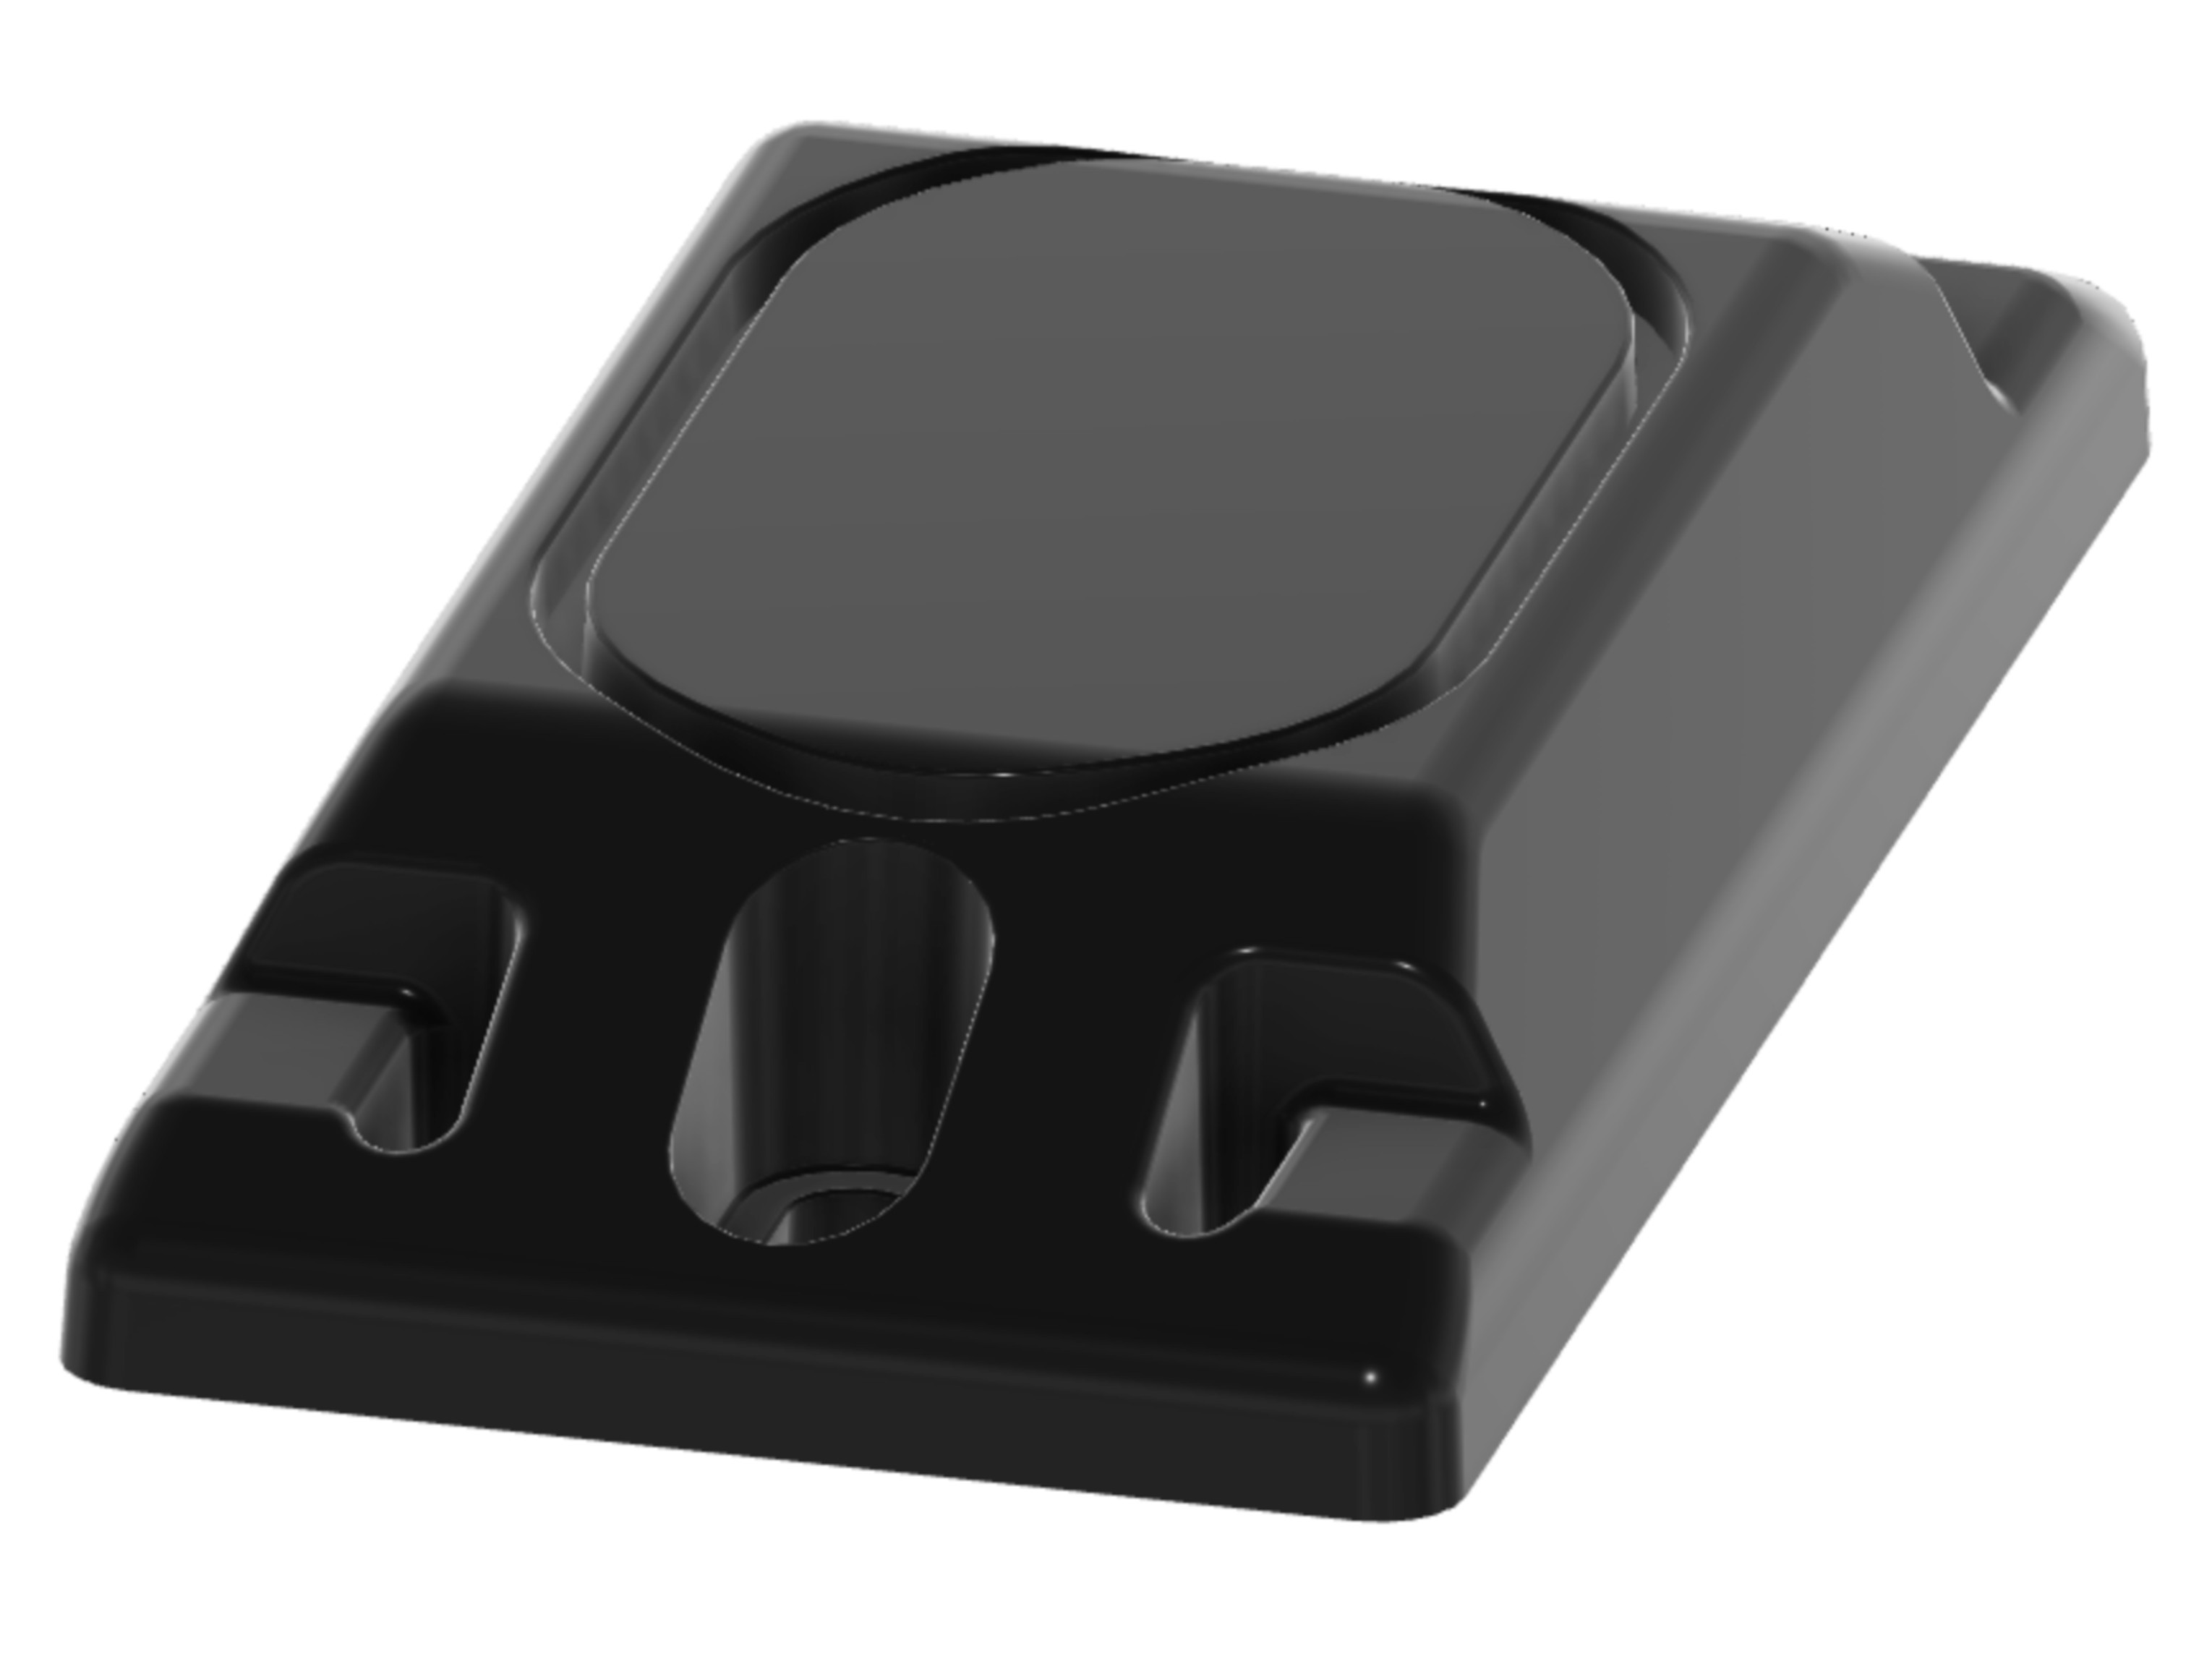
\includegraphics[width=5.5cm]{at_2}
\caption{Walkbase AT-2}
\label{fig:at2}
\end{figure}

\begin{figure}[H]
\centering
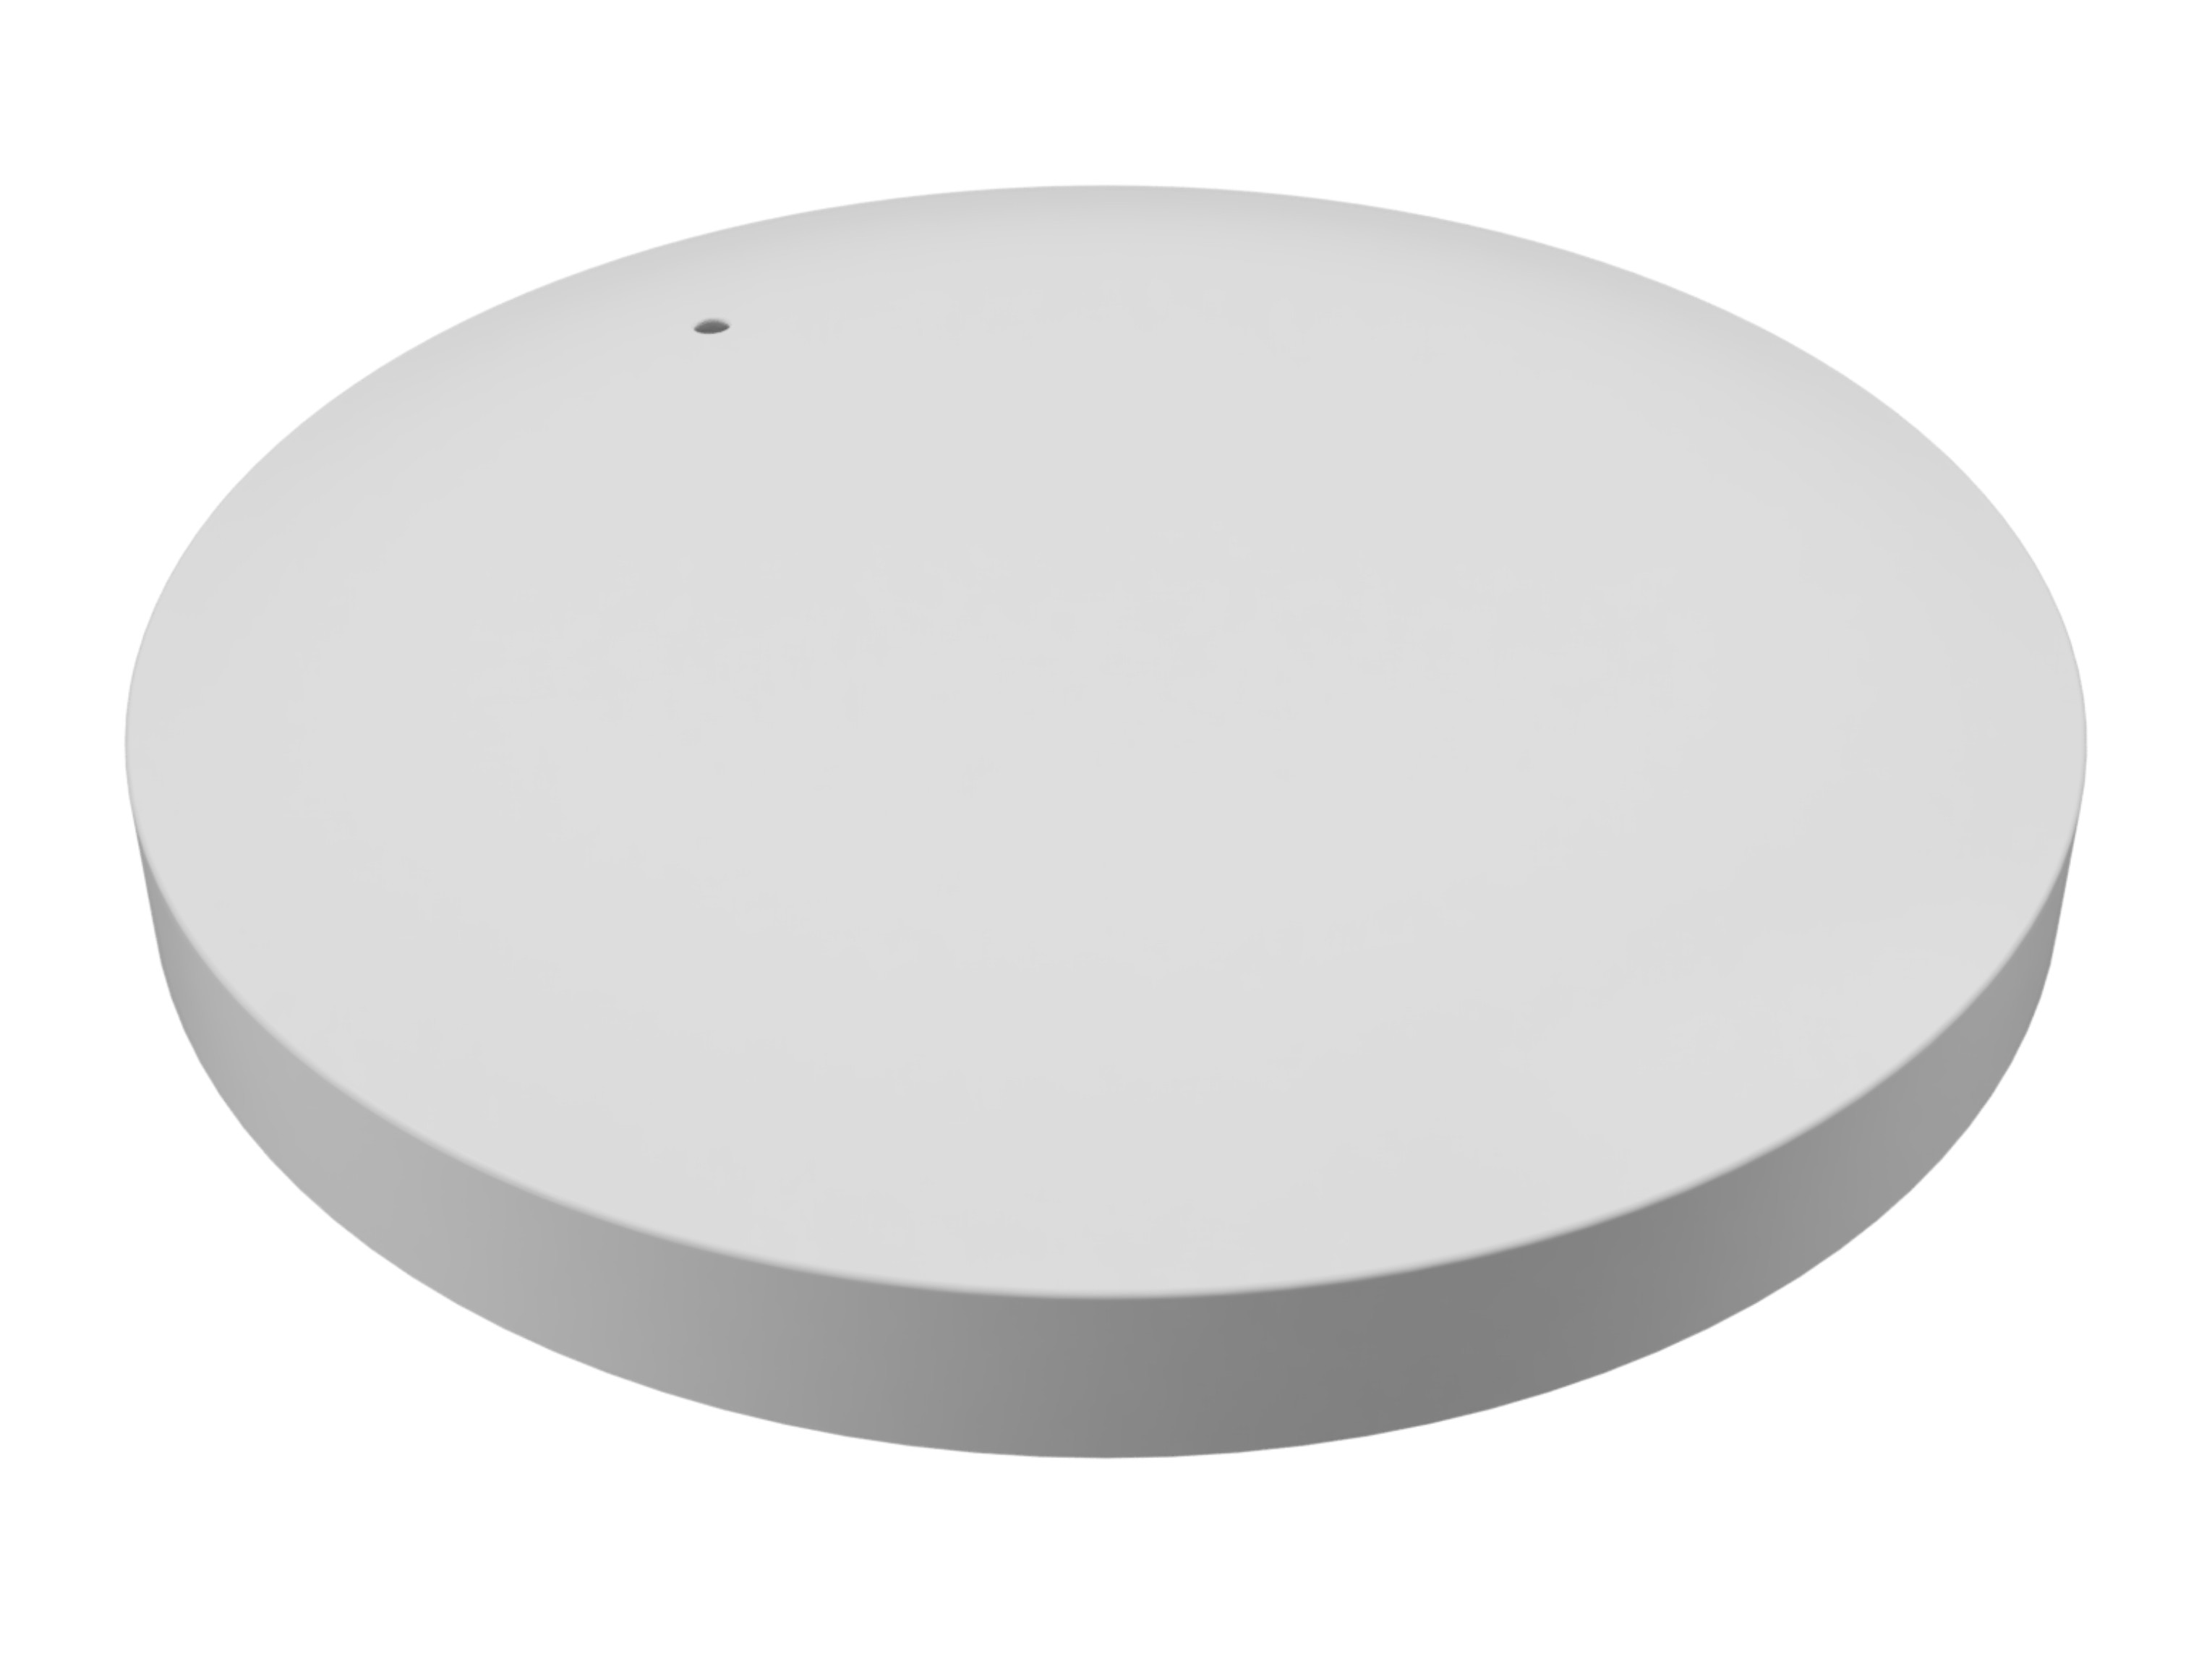
\includegraphics[width=5.5cm]{xr_2_plain}
\caption{Walkbase XR-2}
\label{fig:xr2}
\end{figure}
\end{multicols}

\begin{figure}[H]
\centering
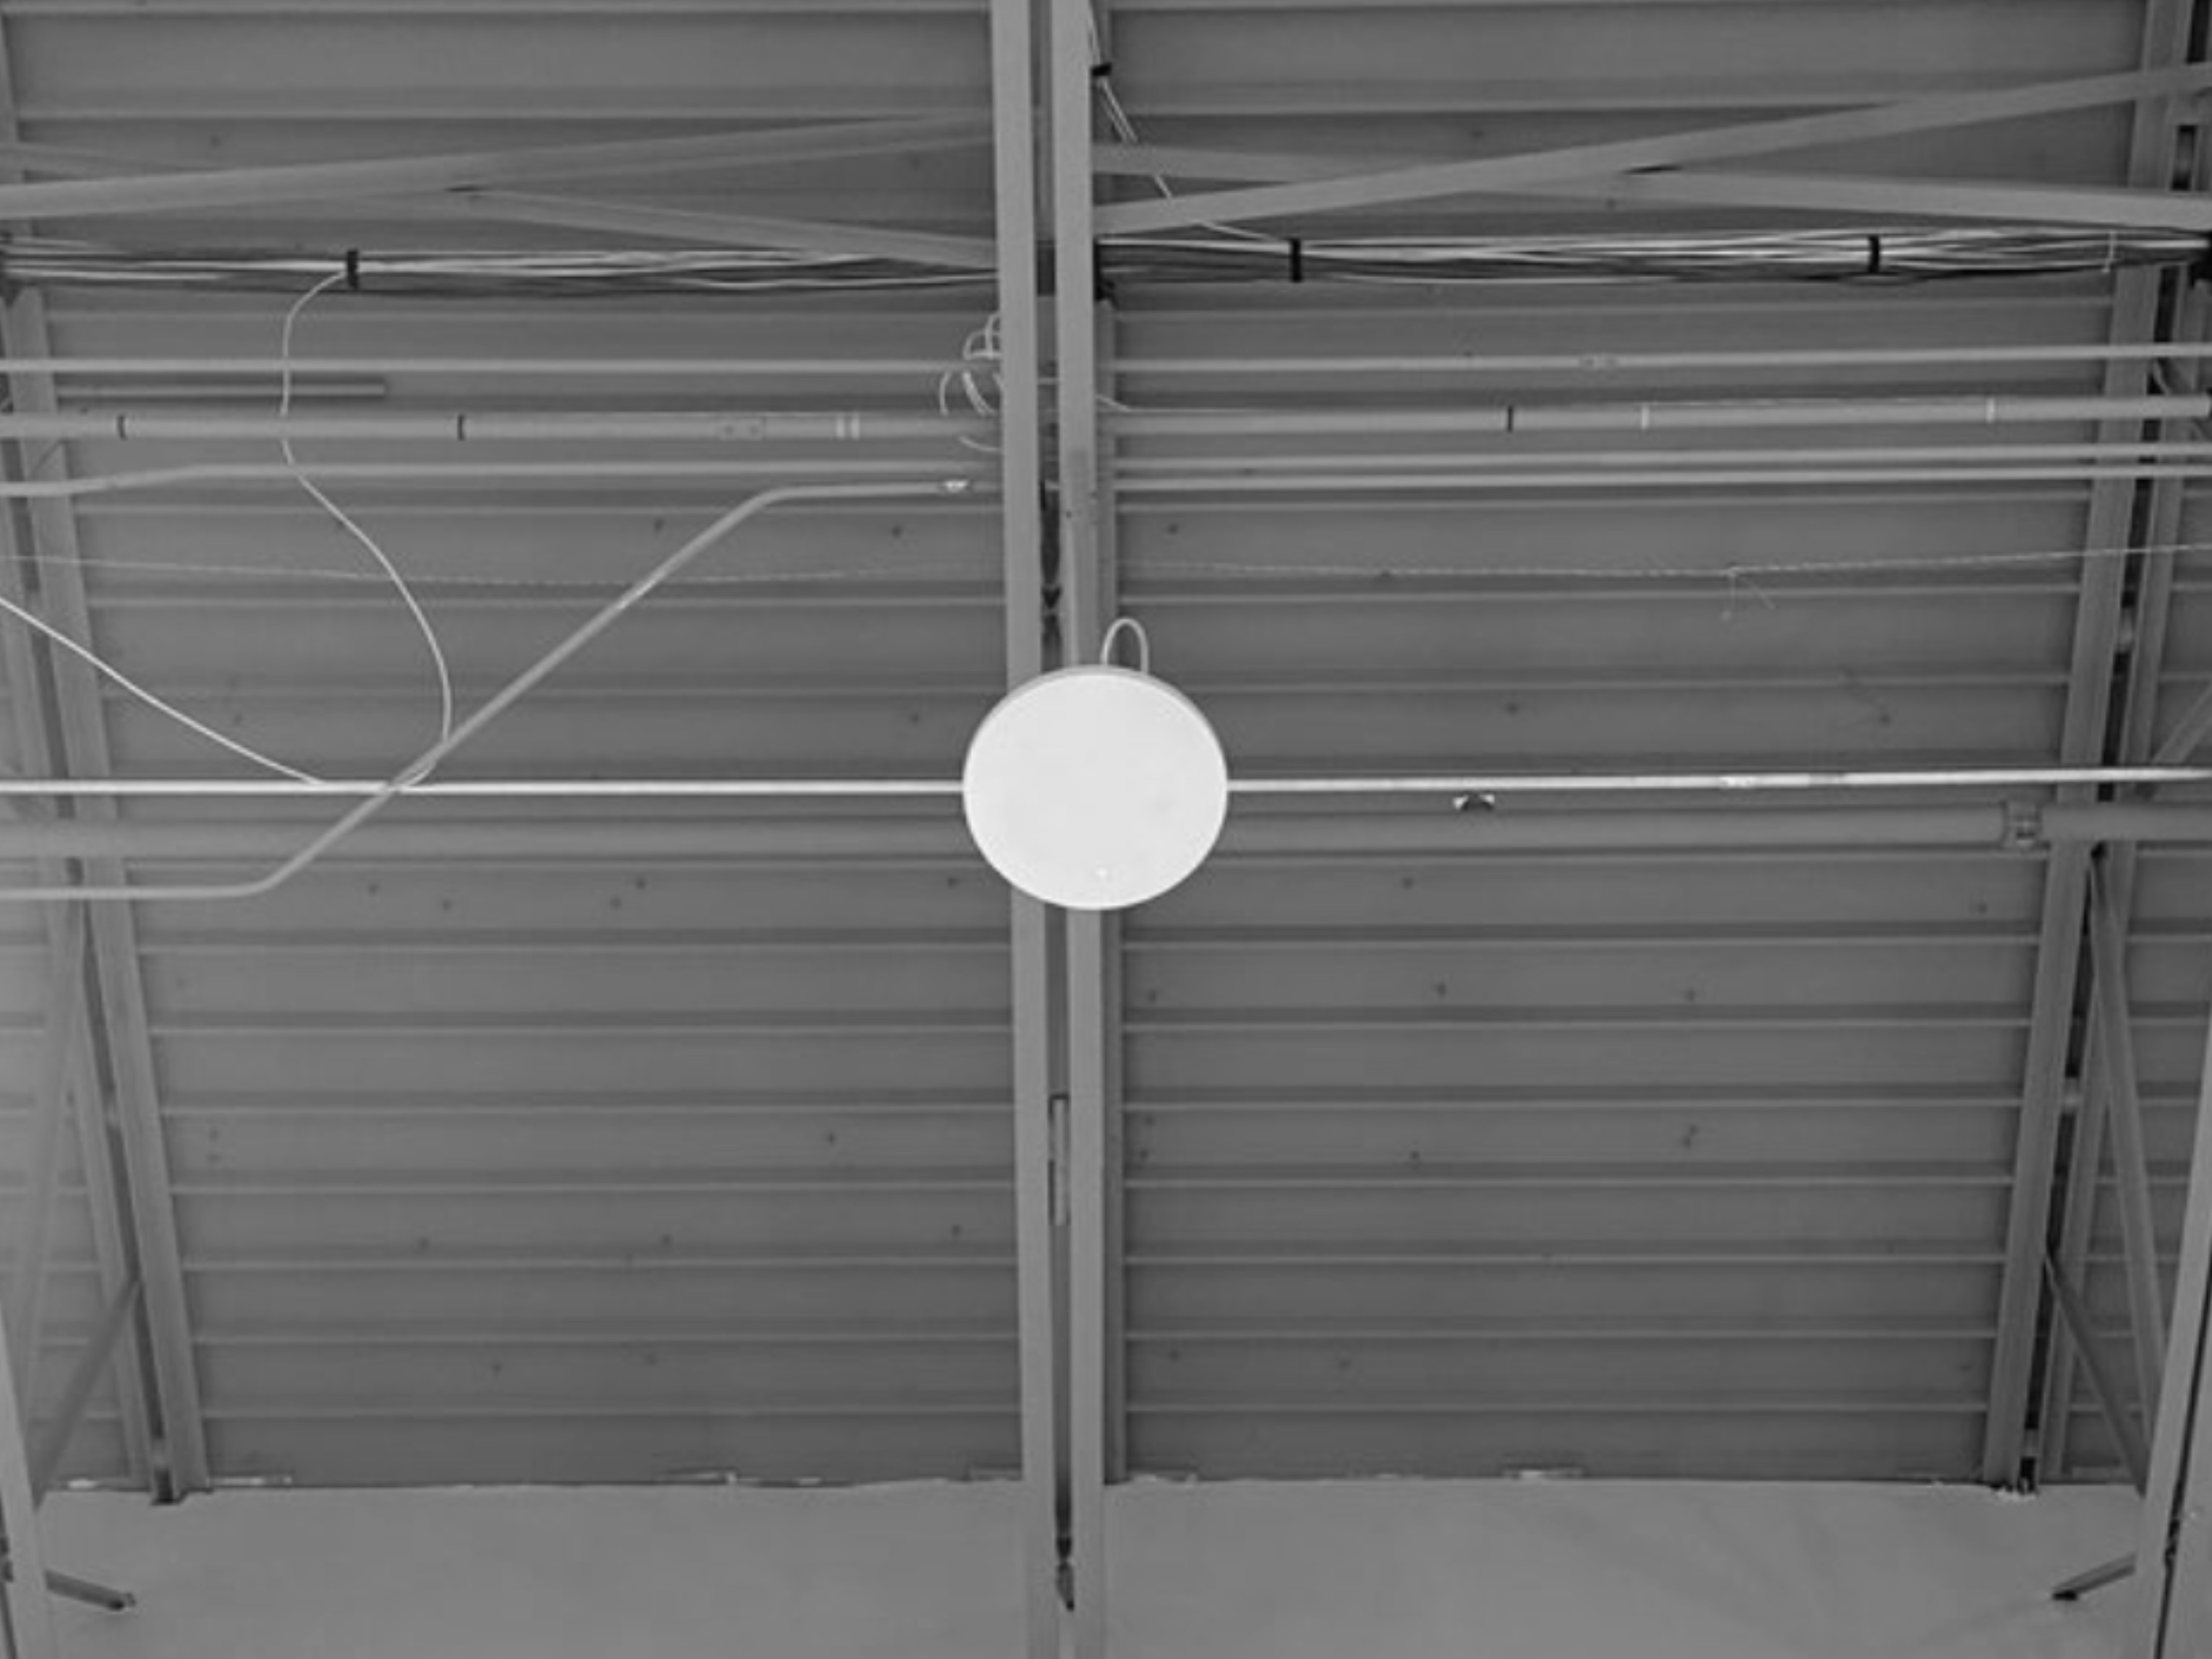
\includegraphics[width=5.5cm]{xr_2_installed}
\caption{Walkbase XR-2 asennettuna}
\label{fig:xr2_installed}
\end{figure}

Koeympäristön pohjapiirustus on esitetty kuvassa \ref{fig:testipolku}. Piirustuksessa XR-2-paikantimet on kuvattu punaisilla ympyröillä ja kuljettu testipolku on merkitty violetilla janalla. Piirustus on luotu käyttäen \texttt{ggplot2}-kirjastoa ja se löytyy RDS-muotoon tallennettuna osoitteesta \newline \url{https://github.com/rintakumpu/progradu/analyysi/R/data/sitemap.RDS}.

\begin{figure}[H]
\centering
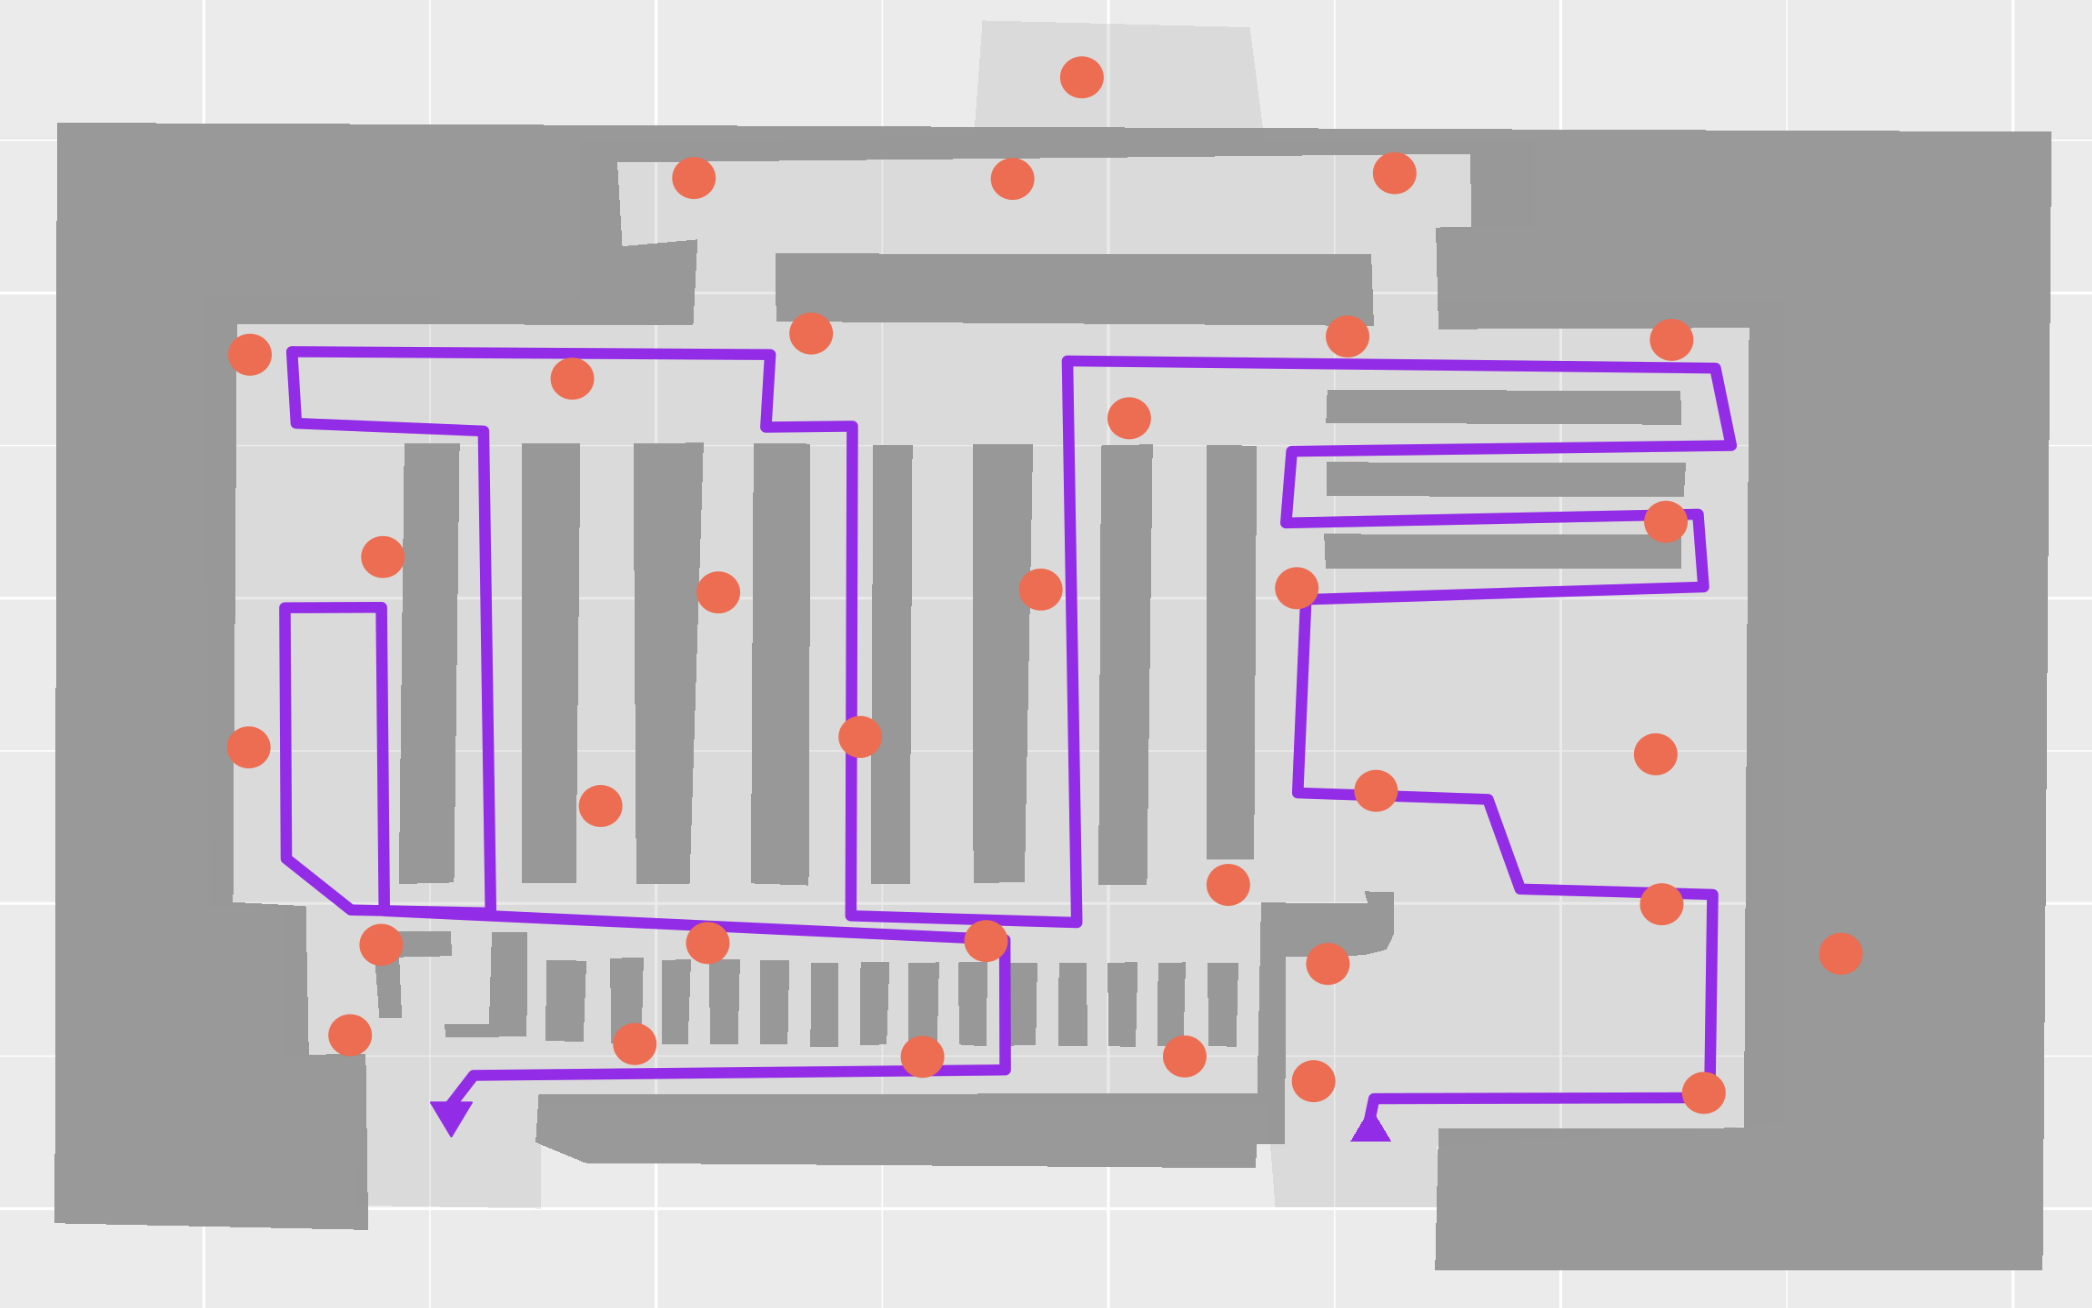
\includegraphics[width=15cm]{testipolku_numeroimaton}
\caption{Koeasetelman pohjapiirustus}
\label{fig:testipolku}
\end{figure}

\noindent Tagi kiinnitettiin ostoskärryyn 1.2 metrin korkeudelle (kts. kuvat \ref{fig:at2_cart} ja \ref{fig:at2_cart2}) ja testipolku käveltiin mahdollisimman tasaisella nopeudella. Data kerättiin aikaan, jolloin testiympäristön käyttöaste oli alhainen. Tällä minimoitiin radiosignaalien tielle osuvien ihmisten vaikutus signaaleihin. Kerätty tulokulma löytyy osoitteesta\newline \url{https://github.com/rintakumpu/progradu/analyysi/data/y.csv}. Pohjapiirustus- ja polkudata löytyy osoitteista\newline \url{https://github.com/rintakumpu/progradu/analyysi/data/exclusion_polygons.csv} (ekskluusiopolygonit),\newline \url{https://github.com/rintakumpu/progradu/analyysi/data/inclusion_polygons.csv} (inkluusiopolygonit) ja\newline \url{https://github.com/rintakumpu/progradu/analyysi/data/test_path.csv} (testipolku). Datassa koordinaatit on valmiiksi interpoloitu metreiksi, jotta testiympäristön tarkkaa sijaintia ei voi paikallistaa koordinaattien perusteella. Interpolointiin käytetty ohjelmakoodi löytyy osoitteesta \newline \url{https://github.com/rintakumpu/progradu/analyysi/R/interpolate_coordinates.R} . Osoitteesta\newline \url{https://github.com/rintakumpu/progradu/analyysi/analyysi.Rmd} löytyy itse analyysikoodin sisältävä R Markdown -muistikirja.

\begin{multicols}{2}
\begin{figure}[H]
\centering
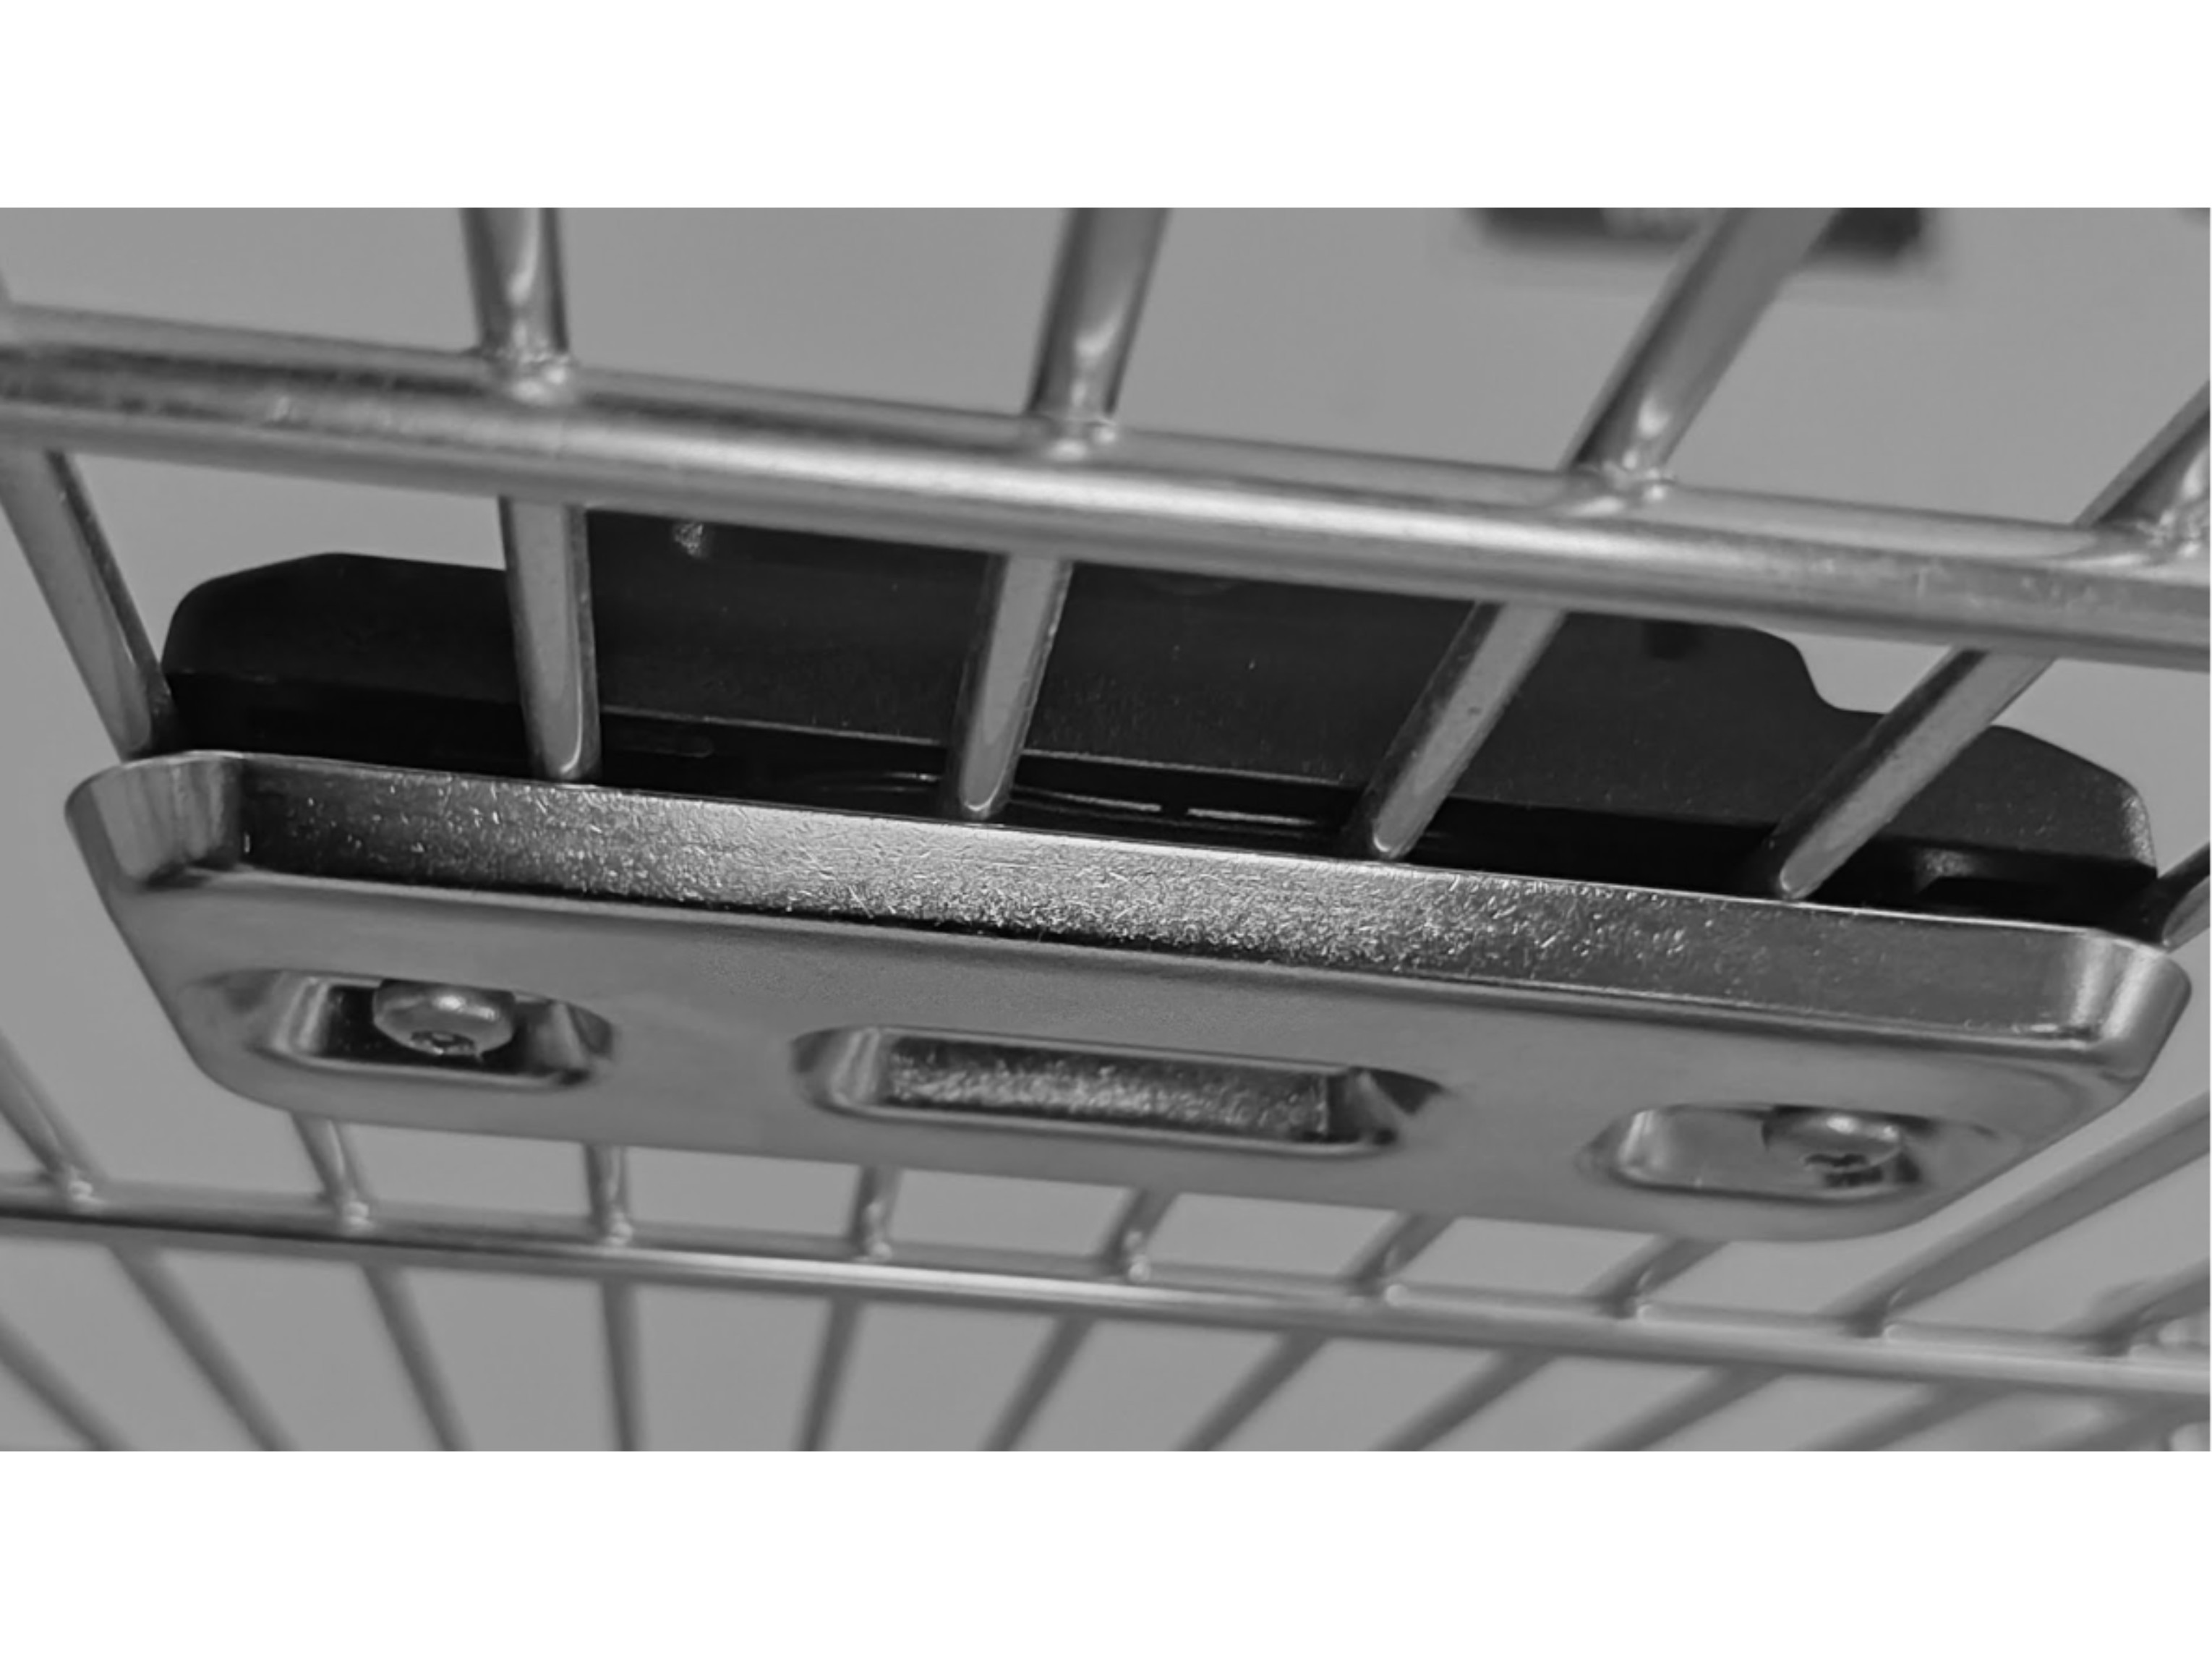
\includegraphics[width=5.5cm]{at_2_cart}
\caption{Walkbase AT-2 kiinnitettynä}
\label{fig:at2_cart}
\end{figure}

\begin{figure}[H]
\centering
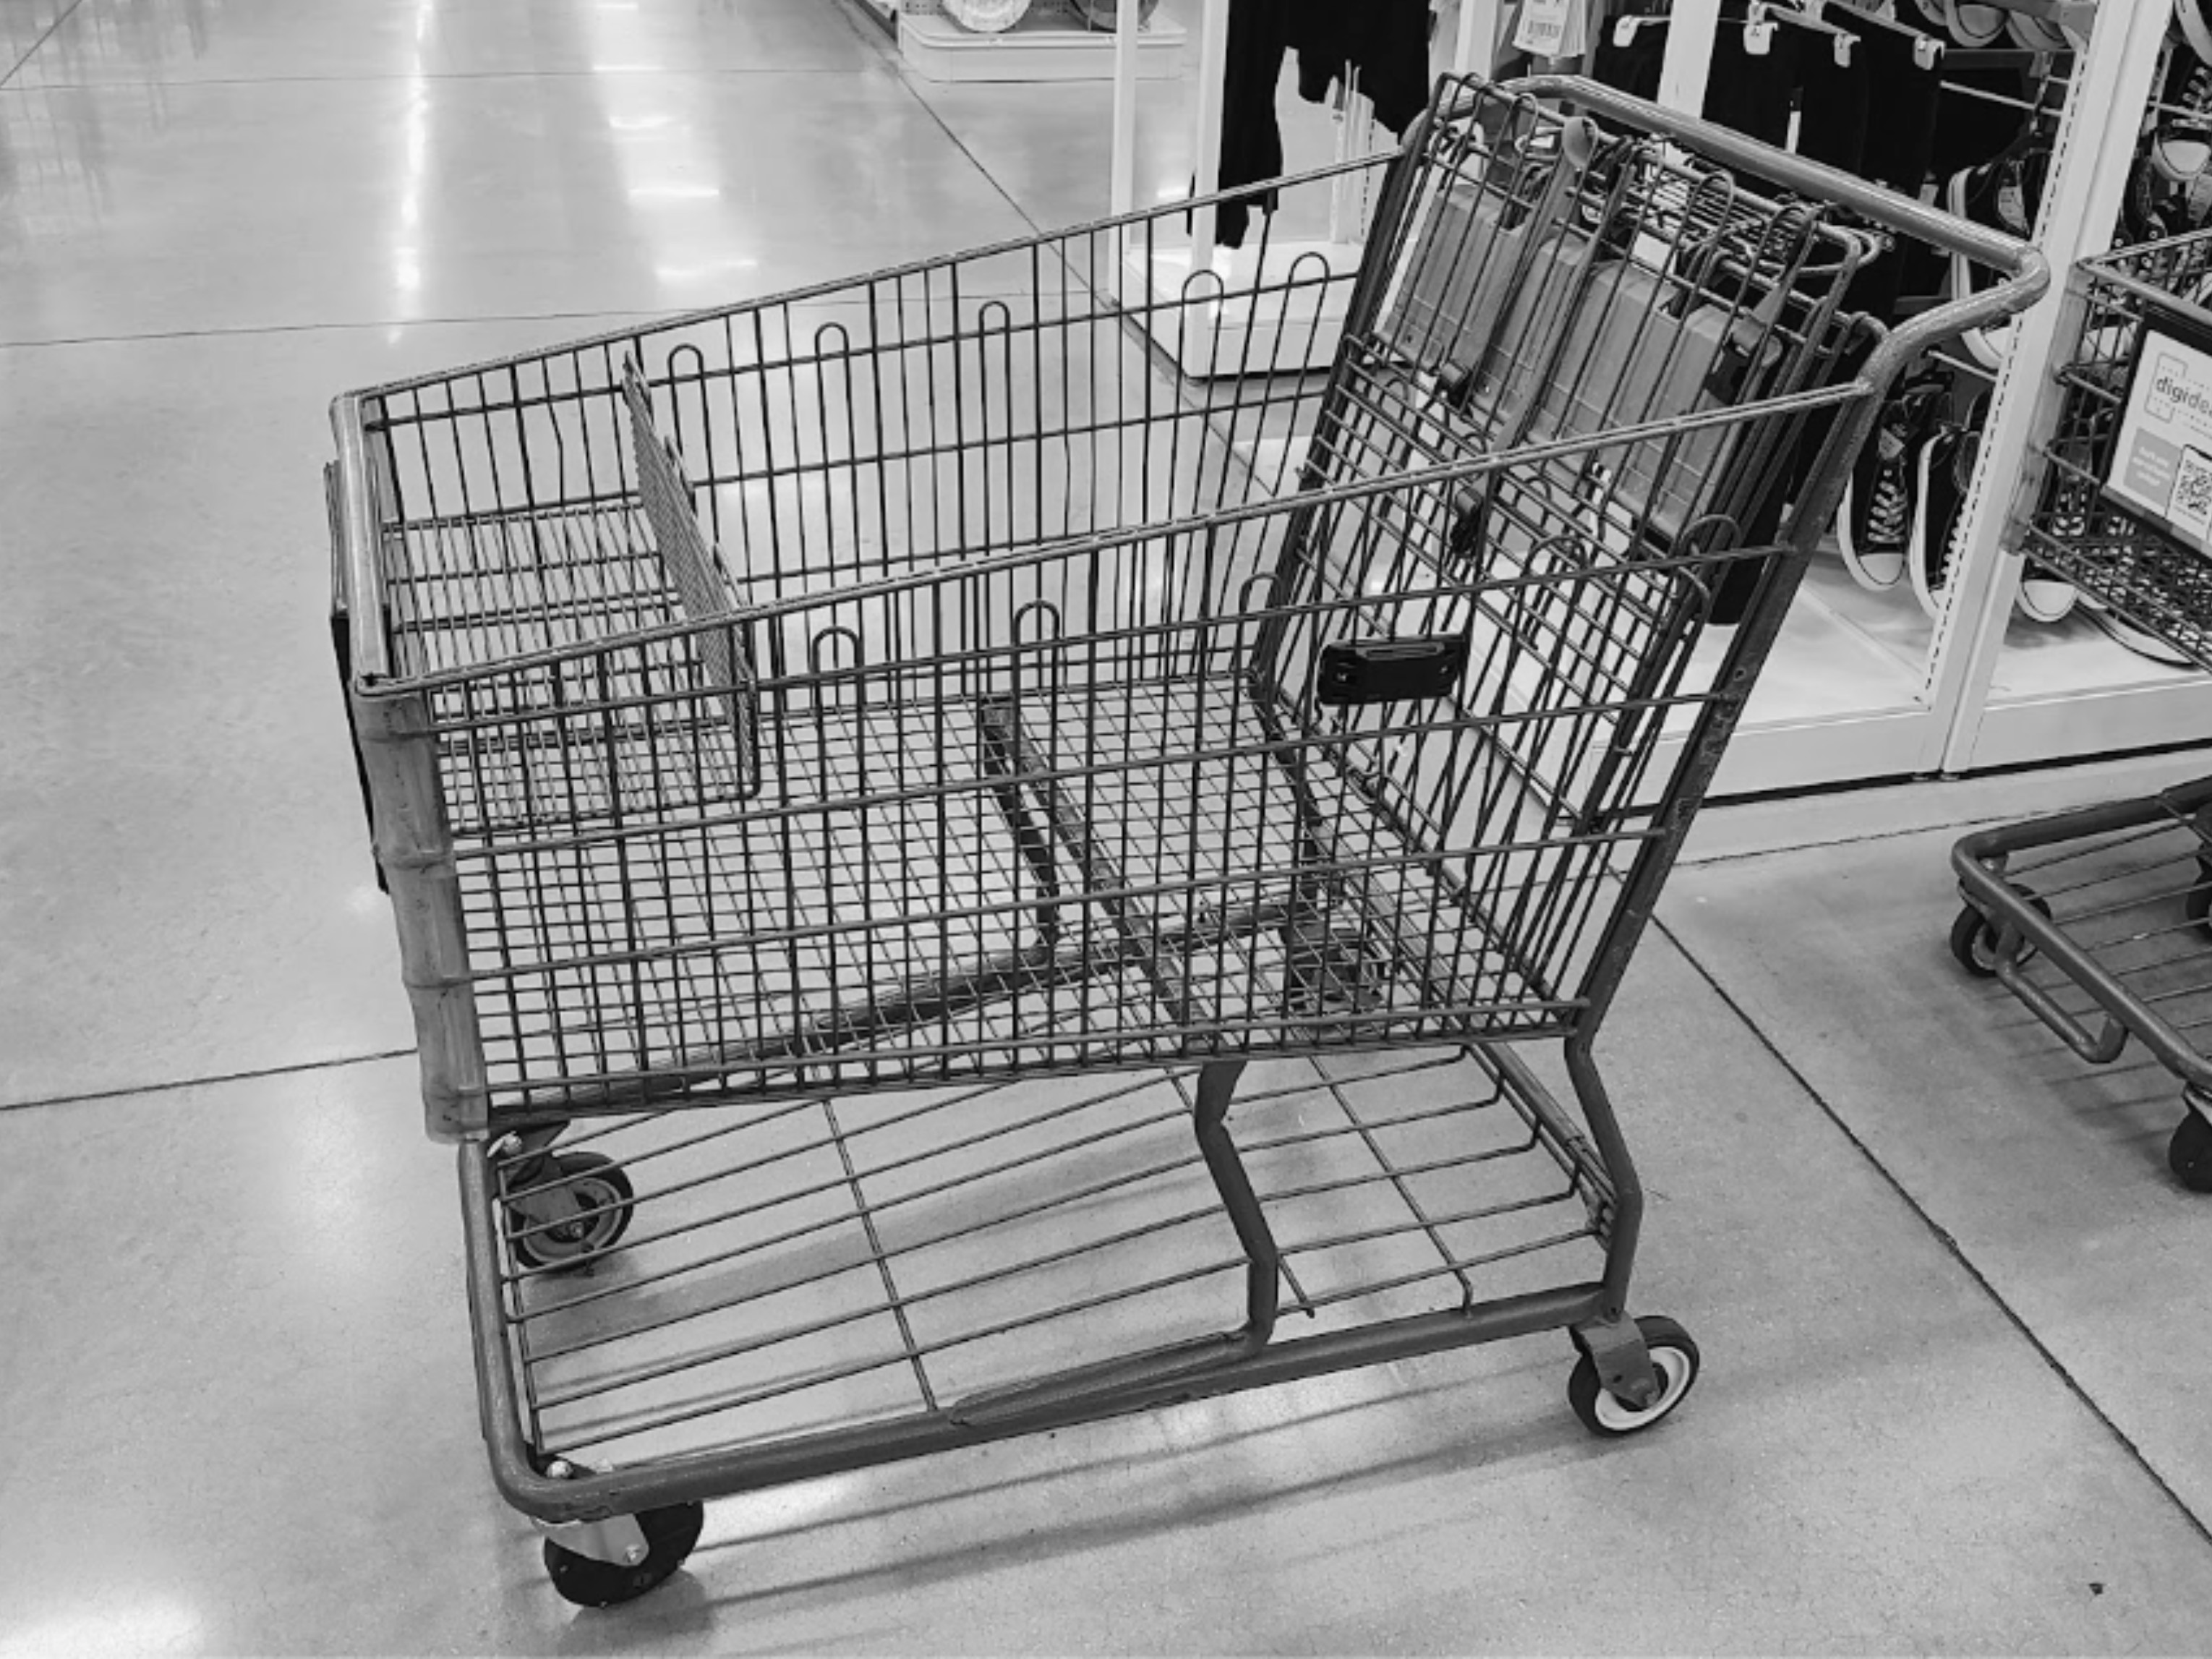
\includegraphics[width=5.5cm]{at_2_cart2}
\caption{Walkbase AT-2 kiinnitettynä}
\label{fig:at2_cart2}
\end{figure}
\end{multicols}

\subsection{Parametrien valinta} \label{parametrien-valinta}

Kokeessa oli tarkoituksena testata kunkin taulukossa \ref{tab:wb-parametrit} esitetyn parametrin vaikutusta paikannusvirheeseen, ajoaikaan sekä varianssiin. Koska kaikkien parametrikombinaatioiden testaaminen ei ollut mahdollista (eikä mielekästä), suoritettiin yllä kerättyyn dataan perustuva paikannus kolmessa vaiheessa. Kussakin vaiheessa paikannusalgoritmi ajettiin jokaisella vaiheeseen liittyvällä suunnitteluparametrikombinaatiolla \(r=30\) kertaa ja tulokset (paikannusvirhe, suoritusaika, varianssi) laskettiin näiden \(30\) ajon aritmeettisena keskiarvona.

Ensimmäisessä vaiheessa tarkasteltiin partikkelien määrän \(N={100,1000,10000}\) sekä uudelleenotannan kynnysarvon \(resampling={0,1/10,2/3,1}\) vaikutusta paikannuskeskivirheeseen. Karttasovitusalgoritmia ei käytetty, kuten ei myöskään prediktiivistä siloitinta eikä signaalin vahvuuden kynnysarvoa. Dynaamisen mallin kohina-arvo \(q=2\) pidettiin vakiona. Ensimmäisessä vaiheessa tarkasteltiin siis \(12\) eri suunnitteluparametrikombinaatiota.

Toisessa vaiheessa valittiin edellisen vaiheen tulosten perusteella parhaimman paikannusvirheen suhteessa suoritusaikaan ja varianssiin tuottava uudelleenotannan kynnysarvo \(resampling\) sekä partikkelien määrä \(N\). Nämä pidettiin vakioarvoisina ja testattiin karttasovitusalgoritmia \emph{map\_matching} \(={T,F}\), karttasovitusalgoritmin rangaistusarvoa \(P={1,100,1000}\) sekä dynaamisen mallin kohina-arvoa \(q={0.75,1.5,2,2.5}\). Signaalin vahvuuden kynnysarvoa ei käytetty, kuten ei käytetty myöskään prediktiivistä siloitinta. Koska rangaistusarvo \(P\) oli käytössä ainoastaan karttasovitusalgoritmia käytettäessä, tarkasteltiin toisessa vaiheessa \(16\) eri suunnitteluparametrikombinaatiota.

Viimeisessä vaiheessa valittiin edellisten vaihdeiden tulosten perusteella parhaimman paikannusvirheen suhteessa suoritusaikaan ja varianssiin tuottavat parametrit testattujen joukosta ja testattiin datan valinnassa käytettävää signaalin vahvuuden kynnysarvoa \emph{rssi\_threshold} \(={-100,-90,-80}\) sekä prediktiivistä siloitinta \emph{smoothing} \(={T,F}\) eli kuutta eri suunnitteluparametrikombinaatiota.

Kaikkien tulosten vertailukohtana käytettiin Pierlot \&al.~artikkelissa ``A New Three Object Triangulation Algorithm Based on the Power Center of Three Circles'' (2011) esittämää ToTal-triangulaatioalgoritmia. \citep{Pierlot-2011} Triangulaatio-algoritmia ei käsitellä tässä tarkemmin, mutta se on esitetty algoritmissa \(\ref{total}\). Algoritmia varten valittiin kunakin aika-askeleella \(k\) ne kolme paikanninta ja kulmahavaintoa, joiden RSSI-arvo oli korkein.

Algoritmi ajettiin RStudion versiossa 2023.09.0+463 R-ohjelmointikielen versiolla 4.2.0. Tietokoneena käytettiin vuoden 2021 mallia olevaa MacBook Pro -kannettavaa, jossa oli Apple M1 Pro -prosessori sekä 32 gigatavua LPDDR5-muistia. Suoritusnopeuden mittaamiseen käytettiin \texttt{microbenchmark}-kirjastoa.

\begin{algorithm}[H]
\label{total}
\DontPrintSemicolon
\SetAlgoShortEnd
\KwResult{Testilaitteen sijaintiestimaatti $(x_R,y_R)$.\;}
\KwData{Kolmen paikantimen koordinaatit $(x_i,y_i)$, $i=\{1,2,3\}$ ja näitä vastaavat vastakkaiset kulmahavainnot $\Phi^\prime_1, \Phi^\prime_2, \Phi^\prime_3$.\;}
\Begin{Lasketaan muokatut koordinaatit \newline
$x^\prime_1=x_1-x_2, \hspace{0.5cm} y^\prime_1=y_1-y_2, \hspace{0.5cm} x^\prime_3=x_3-x_2, \hspace{0.5cm} y^\prime_3=y_3-y_2.$ \;}
\Begin{Lasketaan kotangentit \newline
$T_{12}=\cot(\Phi^\prime_2-\Phi^\prime_1), \hspace{0.5cm} T_{23}=\cot(\Phi^\prime_3-\Phi^\prime_2), \hspace{0.5cm}T_{31}=\frac{1-T_{12}T_{23}}{T_{12}+T_{23}}$.\;}
\Begin{Lasketaan muokatut ympyröiden keskipisteet $(x^\prime_{ij},y^\prime_{ij})$ \newline
$x^\prime_{12}=x^\prime_1+T_{12}y^\prime_1,\hspace{0.5cm}y^\prime_{12}=y^\prime_1-T_{12}x^\prime_1$ \newline $x^\prime_{23}=x^\prime_3-T_{23}y^\prime_3,\hspace{0.5cm}y^\prime_{23}=y^\prime_3+T_{23}x^\prime_3$ \newline
$x^\prime_{31}=(x^\prime_3+x^\prime_1)+T_{31}(y^\prime_3-y^\prime_1),\hspace{0.5cm}y^\prime_{31}=(y^\prime_3+y^\prime_1)-T_{31}(x^\prime_3-x^\prime_1)$.
\;}
\Begin{Lasketaan $k^\prime_{31}=x^\prime_1x^\prime_3+y^\prime_1y^\prime_3+T_{31}(x^\prime_1y^\prime_3-x^\prime_3y^\prime_1).$\;}
\Begin{Lasketaan nimittäjä $D$ (jos $D=0$ palautetaan virhe).\newline
$D=(x^\prime_{12}-x^\prime_{23})(y^\prime_{23}-y^\prime_{31})-(y^\prime_{12}-y^\prime_{23})(x^\prime_{23}-x^\prime_{31})$.\;}
\Begin{Lasketaan ja palautetaan sijaintiestimaatti $(x_R,y_R)$. \newline
$x_R=x_2+\frac{k^\prime_{31}(y^\prime_{12}-y^\prime_{23})}{D}\hspace{0.5cm}y_R=y_2+\frac{k^\prime_{31}(x^\prime_{23}-x^\prime_{12})}{D}$.\;}
\caption{ToTal (Three object Triangulation algorithm)}
\end{algorithm}

\hypertarget{tulokset}{%
\subsection{Tulokset}\label{tulokset}}

Ensimmäisessä vaiheessa suoritettiin paikannus partikkelien määrällä \(N={100,1000,10000}\) sekä uudelleenotannan kynnysarvolla \(resampling={0,1/10,2/3,1}\). Kun kynnysarvo oli \(0\), uudelleenotantaa ei käytetty, jolloin SIR-algoritmin sijaan paikannus suoritettiin bootstrap-suotimella. Kun kynnysarvo oli \(1\), uudelleenotanta suoritettiin jokaisella aika-askeleella. Arvoilla \(1/10\) ja \(2/3\) käytettiin adaptiivista uudelleenotantaa. Tulokset on esitetty kuvassa \(\ref{fig:phase1_results}\) sekä taulukoissa \ref{tab:vaihe-1-tulokset} ja \ref{tab:vaihe-1-tulokset-varianssi}. Ajojen tulokset on esitetty karttapolkuina liitteen A alaluvussa \ref{liite-a-vaihe-1}.

\begin{table}

\caption{\label{tab:vaihe-1-tulokset}Vaiheen 1 tulokset, paikannusvirhe}
\centering
\begin{tabular}[t]{rrrlr}
\toprule
N & resampling & Mediaani (m) & Mediaanin 95\%-luottamusväli & <1m\\
\midrule
100 & 0.00 & 1.93 & {}[1.86, 2.01] & 0.28\\
1000 & 0.00 & 1.05 & {}[1.03, 1.07] & 0.48\\
10000 & 0.00 & 0.88 & {}[0.87, 0.88] & 0.55\\
100 & 0.10 & 0.86 & {}[0.86, 0.87] & 0.57\\
1000 & 0.10 & 0.86 & {}[0.86, 0.87] & 0.57\\
\addlinespace
10000 & 0.10 & 0.86 & {}[0.86, 0.86] & 0.58\\
100 & 0.67 & 0.88 & {}[0.87, 0.89] & 0.56\\
1000 & 0.67 & 0.86 & {}[0.86, 0.87] & 0.58\\
10000 & 0.67 & 0.86 & {}[0.86, 0.86] & 0.58\\
100 & 1.00 & 0.88 & {}[0.87, 0.89] & 0.56\\
\addlinespace
1000 & 1.00 & 0.86 & {}[0.86, 0.86] & 0.58\\
10000 & 1.00 & 0.86 & {}[0.86, 0.86] & 0.58\\
\bottomrule
\end{tabular}
\end{table}

\begin{table}

\caption{\label{tab:vaihe-1-tulokset-varianssi}Vaiheen 1 tulokset, varianssi ja ajoaika}
\centering
\begin{tabular}[t]{rrrrr}
\toprule
N & resampling & Varianssi & MC-varianssi & Ajoaika (s)\\
\midrule
100 & 0.00 & NA & 15.92 & 7.99\\
1000 & 0.00 & NA & 1.41 & 15.92\\
10000 & 0.00 & NA & 0.09 & 1.67\\
100 & 0.10 & 3.28 & 0.10 & 8.11\\
1000 & 0.10 & 1.36 & 0.02 & 16.45\\
\addlinespace
10000 & 0.10 & 0.62 & 0.00 & 1.60\\
100 & 0.67 & 1.09 & 0.06 & 7.79\\
1000 & 0.67 & 0.37 & 0.01 & 15.49\\
10000 & 0.67 & 0.26 & 0.00 & 1.56\\
100 & 1.00 & 1.10 & 0.06 & 7.89\\
\addlinespace
1000 & 1.00 & 0.38 & 0.01 & 15.43\\
10000 & 1.00 & 0.26 & 0.00 & 1.56\\
\bottomrule
\end{tabular}
\end{table}

\clearpage

\begin{figure}[H]
\centering
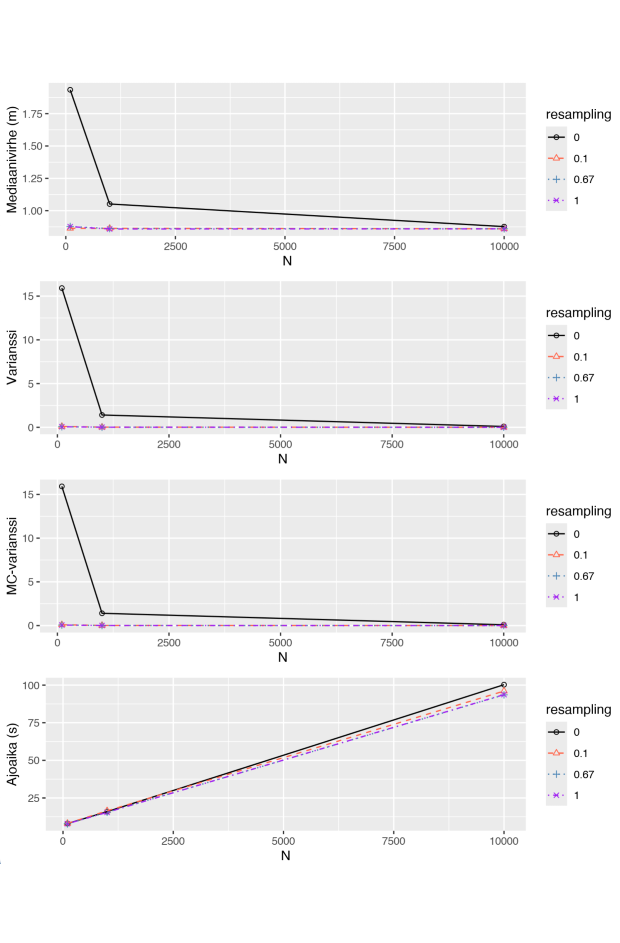
\includegraphics[width=15cm]{phase1_results_vertical_safe}
\caption{Vaiheen 1 tulokset}
\label{fig:phase1_results}
\end{figure}

Ensimmäisen vaiheen tuloksista huomataan, ettei hiukkasten määrällä ole juurikan vaikutusta mediaanipaikannusvirheesen, kun uudelleenotanta on käytössä (so. käytämme SIR-algoritmia). Samoin adaptiivisen uudelleenotannan kynnysarvolla ei ole juurikaan vaikutusta mediaanipaikannusvirheeseen tai ajoaikaan.

Se, ettei partikkelien määrän kasvattaminen automaattisesti paranna paikannustarkkuuta viittaa siihen, että koeasetelma on herkkä priorijakauman valinnalle. Tuloksista huomataan lisäksi, että algoritmin aikakompleksisuus on uudelleenotannasta riipumatta luokkaa \(\mathcal{O}(N)\), kuten tukielman teoriaosassa todettiin. Samoin hiukkasten määrän kasvattaminen pienentää variansseja, kuten teoriaosassa todettiin. MC-varianssia pienentää myös uudelleenotannan käyttäminen.

Koska MC-varianssi on laskettu itse sijaintiestimaateista ja ALvar-varianssi kaikista partikkeleista, on näiden kahden varianssin suuruusluokka eri. Huomataan kuitenkin, että nämä kaksi varianssiestimaattia ovat hyvin korreloituneita, korrelaatiokertoimilla \(\rho_\text{Pearson} \approx 0.86\) ja \(\rho_\text{Spearman} \approx 0.88\). Voidaan siis olettaa ALvar-varianssin estimoivan hyvin hiukkassuotimen todellista varianssia.

Ensimmäisen vaiheen tulosten perusteella valitaan seuraavaan vaiheeseen ne \(N\)- ja \emph{resampling}-parametriarvot, jotka tuottavat parhaimman mediaanipaikannusvirheen. Jos kahden eri paikannusvirheen 95\%-luottamusvälit ovat päällekäiset, valitaan arvoista ensin se, joka tuottaa paremman ALvar-varianssin. Näin päädytään parametriyhdistelmään \(N=10000\), \emph{resampling} \(=2/3\). Koska algoritmin ajoaika 10000 partikkelilla on kuitenkin epäkäytännöllinen, valitaan \(N=1000\), vaikka tämä lisääkin hieman algoritmin varianssia.

Toisessa vaiheessa \(N=1000\) ja \emph{resampling}=\(2/3\) pidettiin vakioarvoisina ja testattiin karttasovitusalgoritmia \emph{map\_matching} \(={T,F}\), karttasovitusalgoritmin rangaistusarvoa \(P={1,100,1000}\) sekä dynaamisen mallin kohina-arvoa \(q={0.75,1.5,2,2.5}\). Signaalin vahvuuden kynnysarvoa ei käytetty, kuten ei käytetty myöskään prediktiivistä siloitinta. Koska rangaistusarvo \(P\) oli käytössä ainoastaan karttasovitusalgoritmia käytettäessä, tarkasteltiin toisessa vaiheessa \(16\) eri suunnitteluparametrikombinaatiota. Tulokset on esitetty kuvassa \(\ref{fig:phase2_results}\) sekä taulukoissa \ref{tab:vaihe-2-tulokset} ja \ref{tab:vaihe-2-tulokset-varianssi}. Ajojen tulokset on esitetty karttapolkuina liitteen A alaluvussa \ref{liite-a-vaihe-2}.

\begin{table}

\caption{\label{tab:vaihe-2-tulokset}Vaiheen 2 tulokset, paikannusvirhe}
\centering
\begin{tabular}[t]{lrrrlr}
\toprule
map\_matching & P & q & Mediaani (m) & Mediaanin 95\%-luottamusväli & <1m\\
\midrule
TRUE & 0 & 0.75 & 0.74 & {}[0.73, 0.74] & 0.66\\
TRUE & 100 & 0.75 & 0.73 & {}[0.72, 0.74] & 0.66\\
TRUE & 1000 & 0.75 & 0.72 & {}[0.71, 0.72] & 0.67\\
TRUE & 0 & 1.50 & 0.72 & {}[0.71, 0.72] & 0.68\\
TRUE & 100 & 1.50 & 0.71 & {}[0.7, 0.72] & 0.68\\
\addlinespace
TRUE & 1000 & 1.50 & 0.69 & {}[0.69, 0.7] & 0.68\\
TRUE & 0 & 2.00 & 0.71 & {}[0.7, 0.72] & 0.68\\
TRUE & 100 & 2.00 & 0.70 & {}[0.69, 0.7] & 0.68\\
TRUE & 1000 & 2.00 & 0.70 & {}[0.69, 0.71] & 0.68\\
TRUE & 0 & 2.50 & 0.71 & {}[0.71, 0.72] & 0.68\\
\addlinespace
TRUE & 100 & 2.50 & 0.69 & {}[0.69, 0.7] & 0.68\\
TRUE & 1000 & 2.50 & 0.70 & {}[0.69, 0.71] & 0.67\\
FALSE & 0 & 0.75 & 0.88 & {}[0.88, 0.89] & 0.57\\
FALSE & 0 & 1.50 & 0.87 & {}[0.87, 0.87] & 0.57\\
FALSE & 0 & 2.00 & 0.86 & {}[0.86, 0.87] & 0.58\\
\addlinespace
FALSE & 0 & 2.50 & 0.86 & {}[0.85, 0.86] & 0.57\\
\bottomrule
\end{tabular}
\end{table}

\begin{table}

\caption{\label{tab:vaihe-2-tulokset-varianssi}Vaiheen 2 tulokset, varianssi ja ajoaika}
\centering
\begin{tabular}[t]{lrrrrr}
\toprule
map\_matching & P & q & Varianssi & MC-varianssi & Ajoaika (s)\\
\midrule
TRUE & 0 & 0.75 & NA & 1.35 & 55.73\\
TRUE & 100 & 0.75 & NA & 2.10 & 65.11\\
TRUE & 1000 & 0.75 & NA & 2.24 & 66.57\\
TRUE & 0 & 1.50 & 0.43 & 0.14 & 57.64\\
TRUE & 100 & 1.50 & 0.43 & 0.58 & 66.86\\
\addlinespace
TRUE & 1000 & 1.50 & 0.47 & 0.92 & 67.85\\
TRUE & 0 & 2.00 & 0.47 & 0.11 & 59.93\\
TRUE & 100 & 2.00 & 0.48 & 0.66 & 68.44\\
TRUE & 1000 & 2.00 & 0.52 & 1.15 & 66.92\\
TRUE & 0 & 2.50 & 0.52 & 0.12 & 57.93\\
\addlinespace
TRUE & 100 & 2.50 & 0.53 & 0.73 & 66.75\\
TRUE & 1000 & 2.50 & 0.58 & 1.08 & 67.41\\
FALSE & 0 & 0.75 & 0.42 & 0.04 & 16.13\\
FALSE & 0 & 1.50 & 0.35 & 0.01 & 16.17\\
FALSE & 0 & 2.00 & 0.37 & 0.01 & 16.07\\
\addlinespace
FALSE & 0 & 2.50 & 0.41 & 0.01 & 16.22\\
\bottomrule
\end{tabular}
\end{table}

\begin{figure}[H]
\centering
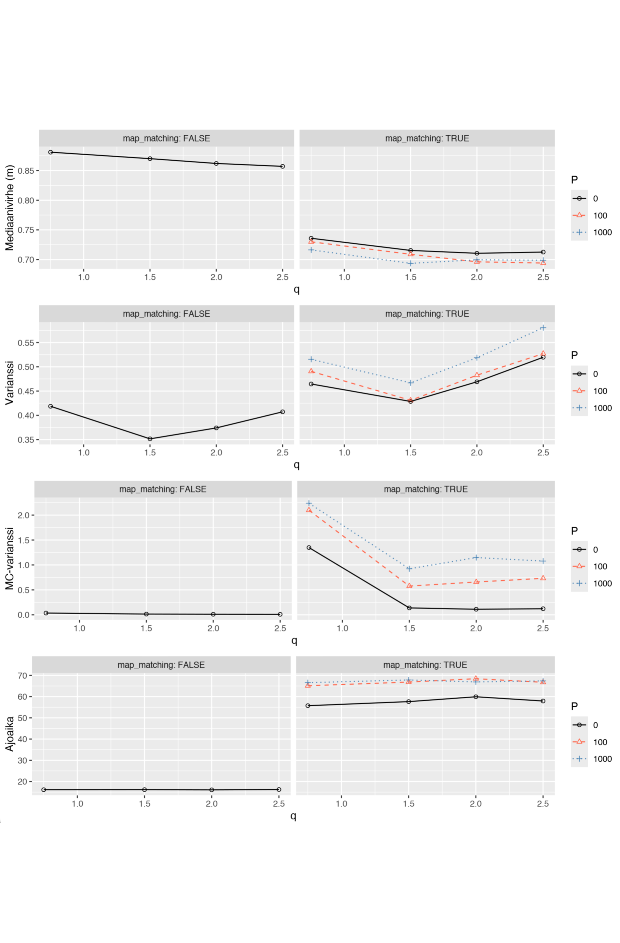
\includegraphics[width=15cm]{phase2_results_vertical_safe}
\caption{Vaiheen 2 tulokset}
\label{fig:phase2_results}
\end{figure}

Toisen vaiheen tuloksista huomataan, että karttasovituksen käyttäminen parantaa paikannusvirhettä. Syy tähän on helppo havaita liitteenä olevista karttapoluista. Paikannus ottaa nyt huomioon sisätilaympäristön, eikä enää luo estimaatteja sijainteihin, jotka ovat fyysisesti mahdottomia. Samoin rangaistusarvo \(P\):n lisääminen parantaa paikannusvirhettä. Tämä on odotettua, sillä isomman rangaistusarvon käyttäminen ei ainoastaan estä fyysisesti mahdottomia sijainteja vaan estää myös fyysisesti mahdottomat siirtymät kahden peräkkäisen sijaintiestimaatin välillä.

Vastaavasti liikemallin kohina-arvon \(q\) pienentäminen parantaa paikannusvirhettä. Liian pienellä \(q\)-arvolla algoritmi ei kuitenkaan enää tutki signaaliympäristöä tarpeeksi hyvin ja paikannusvirhe kasvaa, samoin kasvaa estimaattien MC-varianssi. Optimaalinen kohina-arvo on tulosten perusteella \(q=1.5\). Tämä vastaa myös hyvin kirjallisuudessa esitettyjä keskimääräisiä kävelynopeuksia (kts. esim. \citep{Ho-2016}).

Huomataan lisäksi, että parhaimman paikannusvirheen tuottava rangaistusarvo \(P=1000\) on tutkitun parametriavaruuden reunalla, joten mahdollisesti isommalla \(P\)-arvolla voitaisiin vielä parantaa paikannusvirhettä. Pienempien \(P\)-arvojen paikannusvirheiden luottamusvälit ovat kuitenkin päällekäisiä arvon \(P=1000\) kanssa, joten paikannusvirheeseen saatu lisähyöty ei todennäköisesti olisi tilastollisesti merkityksellistä. Näiden tulosten perusteella valitaan viimeiseen vaiheeseen siis kiinteät arvot \emph{map\_matching}\(=T\), \(P=1000\) sekä \(q=1.5\).

Viimeisessä vaiheessa testattiin datan valinnassa käytettävää signaalin vahvuuden kynnysarvoa \emph{rssi\_threshold} \(={-100,-90,-80}\) sekä prediktiivistä siloitinta \emph{smoothing} \(={T,F}\) eli kuutta eri suunnitteluparametrikombinaatiota. Tulokset on esitetty kuvassa \(\ref{fig:phase3_results}\) sekä taulukoissa \ref{tab:vaihe-3-tulokset} ja \ref{tab:vaihe-3-tulokset-varianssi}. Ajojen tulokset on esitetty karttapolkuina liitteen A alaluvussa \ref{liite-a-vaihe-3}.

\begin{table}

\caption{\label{tab:vaihe-3-tulokset}Vaiheen 3 tulokset, paikannusvirhe}
\centering
\begin{tabular}[t]{rlrlr}
\toprule
rssi\_threshold & smoothing & Mediaani (m) & Mediaanin 95\%-luottamusväli & <1m\\
\midrule
-100 & TRUE & 0.72 & {}[0.72, 0.73] & 0.65\\
-90 & TRUE & 0.73 & {}[0.72, 0.74] & 0.65\\
-80 & TRUE & 0.70 & {}[0.69, 0.71] & 0.62\\
-100 & FALSE & 0.69 & {}[0.69, 0.7] & 0.68\\
-90 & FALSE & 0.70 & {}[0.7, 0.71] & 0.68\\
\addlinespace
-80 & FALSE & 0.70 & {}[0.7, 0.71] & 0.65\\
\bottomrule
\end{tabular}
\end{table}

\begin{table}

\caption{\label{tab:vaihe-3-tulokset-varianssi}Vaiheen 3 tulokset, varianssi ja ajoaika}
\centering
\begin{tabular}[t]{rlrrr}
\toprule
rssi\_threshold & smoothing & Varianssi & MC-varianssi & Ajoaika (s)\\
\midrule
-100 & TRUE & NA & 0.68 & 80.13\\
-90 & TRUE & NA & 0.76 & 78.59\\
-80 & TRUE & NA & 0.86 & 67.85\\
-100 & FALSE & 0.47 & 0.92 & 65.14\\
-90 & FALSE & 0.48 & 0.81 & 64.59\\
\addlinespace
-80 & FALSE & 0.56 & 1.75 & 61.30\\
\bottomrule
\end{tabular}
\end{table}

\clearpage

\begin{figure}[H]
\centering
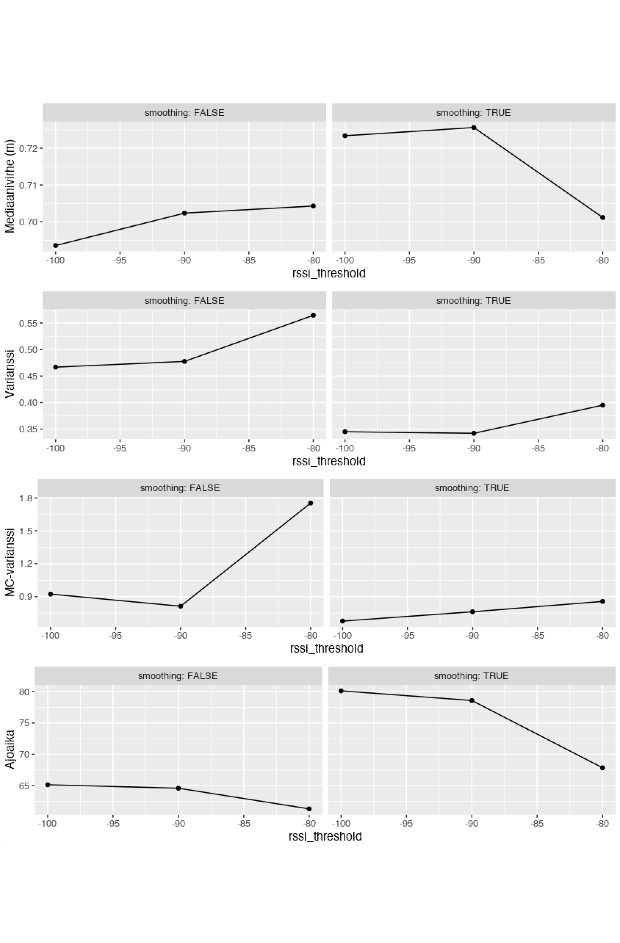
\includegraphics[width=15cm]{phase3_results_vertical_safe}
\caption{Vaiheen 3 tulokset}
\label{fig:phase3_results}
\end{figure}

Tuloksista huomataan, ettei siloittelun tai signaalin vahvuuden kynnysarvon käyttäminen paranna paikannusvirhettä. Siloittelun osalta tämä on odotettua, kun liikemallina on käytetty satunnaiskulkua. Liitteenä olevista karttapoluista kuitenkin huomataan, että siloittelu tuottaa odotetusti sileämpiä polkuja, mikä saattaa olla käytännössä haluttu ominaisuus. Taulukossa \ref{tab:tulokset-final} on esitetty vielä tulosten perusteella valitut suunnitteluparametrit.

\begin{table}

\caption{\label{tab:tulokset-final}Tulosten perusteella valitut suunnitteluparametrit}
\centering
\begin{tabular}[t]{ll}
\toprule
Suunnitteluparametri & Arvo\\
\midrule
N & 1000\\
resampling & 0.67\\
map\_matching & TRUE\\
P & 1000\\
q & 1.5\\
\addlinespace
smoothing & FALSE\\
rssi\_threshold & -120\\
\bottomrule
\end{tabular}
\end{table}

Tulosten perusteella voidaan todeta, että WB-sisätilapaikannusalgoritmi tuottaa halutun paikannusvirheen. Algoritmia ja järjestelmää voitaisiin mahdollisesti edelleen parantaa esimerkiksi hyödyntämällä paremmin tagin kiihtyvyysmittarin tuottamaa dataa informatiivisen liikemallin luomisessa. Vastaavasti datan valinta voitaisiin suorittaa esimerkiksi niin, että datasta poistettaisiin kullakin aika-askeleella ne kulmahavainnot, jotka poikkeavat kulmahavaintojen suuntakonsensuksesta.

Liitteenä olevia polkuja tarkastelemalla huomataan, että nyt toteutetun algoritmin sijantiestimaatilla on taipumus jäädä osassa testiympäristöä jälkeen itse tagin sijainnista. Tätä ongelmaa voitaisiin mahdollisesti lieventää käyttämällä esimerkiksi Yi Chenging \&al artikkelissa ``Improved Particle Filter Algorithm for Multi-Target Detection and Tracking'' (2024) \citep{Cheng-2024} esittämää menetelmää, jossa partikkelit jaetaan ns. seurantahiukkasiin sekä etsintähiukkasiin, joista ainoastaan edellisiä käytetään sijaintiestimaatin luomisessa ja jälkimmäisten annetaan liikkua suuremmilla kohina-arvoilla. Näin mahdollistetaan satunnaiskulkumallilla laajempi signaaliavaruuden tutkinta ja nopeampi ongelmatilanteista toipuminen ilman, että sijaintiestimaatit kärsivät liikemalliin lisätystä kohinasta.

\hypertarget{lopuksi}{%
\chapter{Lopuksi}\label{lopuksi}}

Tässä tutkielmassa on esitetty pääpiirteittäin hiukkassuodin- ja hiukkassiloitinalgoritmien teoria Bayesilaisessa tilastotieteellisessä viitekehyksessä. Tutkielmassa on lisäksi käyty läpi uudelleenotantaa efektiivisen otoskoon perusteella hyödyntävä SIR-suodinalgoritmi sekä käsitelty algoritmin varianssin estimointia. Tutkielmassa on myös esitetty SIR-algoritmin parametrien valintaan, suorituskykyyn sekä konvergenssiin liittyviä tuloksia.

Tutkielmassa on lisäksi esitetty WB-sisätilapaikannusalgoritmi, joka toteuttaa SIR-algoritmin, varianssin estimoinnin sekä hyödyntää sisätilapaikannuksen karttasovitusalgoritmia. Tutkielmassa on lopuksi tarkasteltu miten eri suunnitteluparametrien valinnat vaikuttavat tämän algoritmin suorituskykyyn kattavan ja todelliseen ongelmaan sekä dataan perustuvan paikannusesimerkin avulla.

\hypertarget{liite-a---karttapolut}{%
\chapter*{Liite A - Karttapolut}\label{liite-a---karttapolut}}
\addcontentsline{toc}{chapter}{Liite A - Karttapolut}

Liite sisältää tutkielmaan tulososioon liittyvät karttapolut. Kukin kartta käsittää \(r=30\) ajoa kullakin suunnitteluparametrikombinaatiolla. Karttojen otsikossa on mainittu ainoastaan testatut suunnitteluparametrit, vakioarvoiset parametrit on esitetty luvussa \ref{tulokset}.

\section{Vaihe 1} \label{liite-a-vaihe-1}

\section{Vaihe 2} \label{liite-a-vaihe-2}

\section{Vaihe 3} \label{liite-a-vaihe-3}

  \bibliography{packages.bib,lahteet.bib}

\end{document}
